\documentclass[11pt]{article}
% Shared preamble
\usepackage[papersize={8.5in,11in},textwidth=437pt,textheight=634pt,hcentering,top=81pt,headsep=22pt,headheight=16pt]{geometry}
\usepackage[T1]{fontenc}
\usepackage{lmodern}
\usepackage{mathtools,amssymb,amsthm}
\usepackage{microtype}
\usepackage{booktabs,array}
\usepackage[font=small,labelfont=bf,labelsep=period]{caption}
\usepackage[shortlabels]{enumitem}
\usepackage{needspace}
\usepackage{tikz}
\usetikzlibrary{calc,positioning,arrows.meta}
\definecolor{ink}{HTML}{213650}
\definecolor{sea}{HTML}{19706F}
\definecolor{rust}{HTML}{AA5034}
\usepackage[numbers,sort&compress]{natbib}
\renewcommand\bibfont{\small}
\usepackage[nottoc,notlof,notlot]{tocbibind}
\usepackage{fancyhdr}
\usepackage{url}
\usepackage[colorlinks,linkcolor=ink,citecolor=sea,urlcolor=ink,psdextra]{hyperref}
\usepackage{bookmark}

\fancyhf{}
\newcommand\shorttitle{OpenAI}
\fancyhead[L]{\small\scshape\shorttitle}
\fancyhead[R]{\small\thepage}
\renewcommand\headrulewidth{0pt}
\pagestyle{fancy}
\newcommand{\articletitle}[2]{\title{\fontsize{20}{24}\selectfont\bfseries\color{ink}#1}\renewcommand\shorttitle{#2}%
  \hypersetup{pdftitle={#1},pdfauthor={OpenAI}}}
\author{OpenAI}
\date{November 24, 2026}
\setcounter{tocdepth}{1}

\newtheorem{theorem}{Theorem}[section]
\newtheorem{lemma}[theorem]{Lemma}
\newtheorem{claim}[theorem]{Claim}
\newtheorem{corollary}[theorem]{Corollary}
\newtheorem{proposition}[theorem]{Proposition}
\theoremstyle{definition}
\newtheorem{definition}[theorem]{Definition}
\newtheorem{remark}[theorem]{Remark}
\newtheorem{example}[theorem]{Example}
\numberwithin{equation}{section}
\emergencystretch=1em
\clubpenalty=3500
\widowpenalty=3500
\raggedbottom

% For numbers of results in companion papers
\makeatletter
\newcommand\ext[2]{\@ifundefined{ref@#1:#2}{??\@latex@warning{Undefined companion label #1:#2}}{\csname ref@#1:#2\endcsname}}
\newcommand\extdef[3]{\@namedef{ref@#1:#2}{#3}}
\makeatother
\input{locators}

\newcommand\titlebreak{\texorpdfstring{\\}{}}
\settocbibname{References}

% Lightweight contents, with numbered bookmarks
\bookmarksetup{numbered}
\makeatletter
\renewcommand\@pnumwidth{2.1em}
\renewcommand\@dotsep{12}
\renewcommand*\l@section[2]{\addvspace{.35em}\@dottedtocline{1}{\z@}{2em}{#1\nobreak\hspace{.5em}}{#2}}
\makeatother

\articletitle{Euclidean geometry \titlebreak in the asymptotic spectrum of tensors}{Euclidean geometry in the asymptotic spectrum}
\newcommand{\paperidentifier}{Euclidean-geometry-in-the-asymptotic-spectrum-of-tensors-November-24-2026}
\hypersetup{pdfsubject={\paperidentifier}}

\begin{document}
\maketitle
\begin{abstract}
Over any field, we assign costs to tensors with indices placed in a real
Hilbert space so that a bit shared by two sites costs exactly their distance.
On each finite set of two or more sites, the costs are scaled logarithms of
invariants that add under direct sums, multiply under tensor products, and
cannot increase under local linear maps. In every such system, a bit shared
among finitely many sites costs the mean width of their convex hull,
normalized to give a segment its length. For a triangle this is half its
perimeter. Companion papers use these costs to compare tensors with the
networks that produce them, yielding lower bounds for arithmetic circuits
and an exponential bound on the size of sunflower-free set families.
\end{abstract}

\section{Introduction}

Place the two indices of the tensor
\(e_0\otimes e_0+e_1\otimes e_1\) at sites \(x\) and \(y\).
The indices carry the same binary label. This tensor acts as a
\emph{wire} because contracting its first index with a two-dimensional index of
another tensor moves that index from \(x\) to \(y\). Can an invariant
of placed tensors assign the wire itself its Euclidean length? We ask
for one assignment that works simultaneously for all pairs of sites
and respects local linear maps on all tensors.

Strassen's asymptotic spectrum supplies the algebraic rules for such an
invariant~\cite{Strassen1988}. A \emph{spectral point} on a fixed finite
set of two or more sites assigns a nonnegative number \(F(T)\) to each tensor.
Applying a linear map at each site is a \emph{restriction} and cannot
increase \(F\). Tensor products multiply its values, and direct sums
add them. Here a direct sum places the two tensors in separate blocks at
every site. The normalization is \(F(0)=0\) and \(F(1)=1\).
Taking a logarithm turns multiplication into addition. We call a
positive multiple of \(\log_2 F(T)\) a \emph{price}, with
\(\log_2 0=-\infty\). Independent wires
then have additive prices, and contracting wires produces a tensor whose price is at most the sum of
their prices.

For a finite nonempty set \(S\) of sites, write
\(\Delta_S(q)=\sum_{j=1}^q\bigotimes_{s\in S}e_j\) for the tensor
that shares one \(q\)-valued label among those sites. Let \(W(S)\)
denote the \emph{mean width} of their convex hull. It is the average
length of a one-dimensional projection over uniformly distributed
directions in the affine span, multiplied by a constant that gives
a segment its length. A singleton has width zero. Equivalently, for a standard Gaussian vector \(g\)
in the finite-dimensional span of \(S\),
\[
                   W(S)=\sqrt{2\pi}\,\mathbb E\max_{s\in S}\langle g,s\rangle .
\]
Translating all the sites adds a centered Gaussian to the maximum and
hence leaves its expectation unchanged.

\begin{theorem}[Euclidean prices]\label{thm:main}
Let \(k\) be any field and \(K\) any real Hilbert space. There is a
compatible assignment \(H(T;x)\) to every tensor over \(k\) and every
placement \(x=(x_1,\ldots,x_r)\) of its indices in \(K\) with the
following properties.
\begin{enumerate}[leftmargin=*,itemsep=.35ex]
\item A binary wire between \(u\) and \(v\) costs \(\|u-v\|\).
More generally, \(H(\Delta_S(q))=W(S)\log_2 q\) for every nonempty
finite \(S\subset K\) and every integer \(q\ge1\).
\item For each finite set \(S\subset K\) of positive diameter there is
a spectral point \(F_S\) such that \(H(T;x)=W(S)\log_2 F_S(T)\) for
every tensor placed in \(S\). In evaluating \(F_S\), group the
indices at each site and adjoin a one-dimensional factor at each unused
site. Compatibility means that enlarging \(S\) leaves \(H(T;x)\)
unchanged.
\item For each nonzero \(T\), the price depends on \(x\) only through
the labeled distances \(\|x_i-x_j\|\), and \(H(T;tx)=tH(T;x)\) for
\(t\ge0\).
\end{enumerate}
\end{theorem}

\begin{figure}[htbp]
\centering
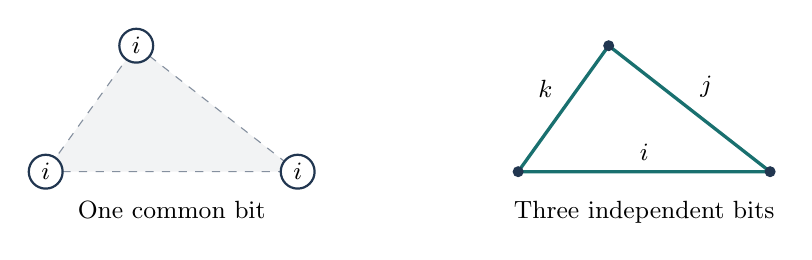
\begin{tikzpicture}[font=\small, site/.style={circle,inner sep=2pt,
        fill=white,draw=ink,thick}, edge/.style={draw=sea,very thick}]
\begin{scope}
\coordinate (a) at (0,0); \coordinate (b) at (3.2,0); \coordinate (c) at (1.15,1.6);
\filldraw[fill=ink!6,draw=ink!55,dashed] (a)--(b)--(c)--cycle;
\foreach \v in {a,b,c} \node[site] at (\v) {\(i\)};
\node[below=7pt] at (1.6,0) {One common bit};
\end{scope}
\begin{scope}[xshift=6.0cm]
\coordinate (a) at (0,0); \coordinate (b) at (3.2,0); \coordinate (c) at (1.15,1.6);
\draw[edge] (a)--node[midway,above]{\(i\)}(b)--node[midway,above right]{\(j\)}(c)--node[midway,above left]{\(k\)}cycle;
\foreach \v in {a,b,c} \fill[ink] (\v) circle (2pt);
\node[below=7pt] at (1.6,0) {Three independent bits};
\end{scope}
\end{tikzpicture}
\caption{Two tensors on the same triangle of perimeter \(P\). On the
left, the tensor is supported on triples \((i,i,i)\) and costs \(P/2\).
On the right, each edge carries its own binary index. The tensor product
of the three wires costs \(P\).}
\label{fig:triangle}
\end{figure}

The shared-label formula is forced. Every compatible spectral system
realizing the wire distances on a whole Euclidean flat gives the same
value for \(\Delta_S(q)\) (Theorem~\ref{thm:flatlaw}). For planar sites
whose convex hull is a polygon this value per bit is half the hull's
perimeter. Figure~\ref{fig:triangle} illustrates why it matters which
labels are shared. The formula also controls tensors carrying a common
label alongside other data. If a tensor already carries that label on
\(S\), appending a copy at \(z\) increases its price by at most
\((W(S\cup\{z\})-W(S))\log_2 q\) (Proposition~\ref{lem:submod}).
In particular, a copy can be inserted anywhere on the segment joining
two existing copies at zero additional price. For arbitrary nonzero
\(T\), the chosen price is a seminorm on placements modulo common
translation. Applying a linear contraction to every site can only
decrease this price (Section~\ref{sec:hilbert}).

\subsection{Why a spectral point is needed}

Across a cut of the sites, a tensor can be viewed as a matrix, and its
matrix rank is a spectral point. A binary wire has rank two across a
cut separating its endpoints and rank one across every other cut.
Thus an average of log ranks measures how frequently the endpoints are
separated. Integrating over hyperplane cuts in Euclidean space recovers
the length of a wire. For each direction, the thresholds that split \(S\) form an interval
whose length is the width of the projection. Integrating these
lengths recovers the mean width for the shared label.

The difficulty is extending these evaluations to a spectral point on
\emph{all} tensors at the sites. For a small example, divide the four
corners of a square by its vertical and horizontal midlines. Let \(U\)
be a horizontal wire and \(V\) a vertical wire. Their matrix ranks
across the two cuts are \((2,1)\) and \((1,2)\), respectively. The
geometric mean of the ranks is \(\sqrt2\) for each tensor, but on their
direct sum it is \(\sqrt{3\cdot3}=3\). Additivity would give
\(2\sqrt2\). Even on wires, the metric obtained by averaging these two
cuts is a rescaled Hamming square and violates the four-point inequality
\eqref{eq:cur-quad} for spectral prices.

Direct sums matter for network constructions. If two tensors have the
same output spaces, their ordinary sum is a restriction of their direct
sum. The price of a sum of \(m\) alternatives on sites \(S\) is
therefore at most their largest price plus \(W(S)\log_2 m\).
Compatibility lets us use this bound even when the alternatives use
different auxiliary sites. For a single graph tensor, the tensor
product of its edge wires~\cite{cvzgraph}, each edge of dimension \(q\)
contributes its length times \(\log_2 q\). The wire formula gives the exact price of the graph tensor, and the
sum bound controls the price of alternative wirings.

\subsection{Relation to earlier work}

Strassen introduced the asymptotic spectrum to study transformations of
large tensor powers, motivated in particular by matrix multiplication
\cite{Strassen87,Strassen1988}. Comparison at all spectral points
characterizes asymptotic restriction. The difficult part in concrete
applications is to understand which evaluations can occur together.
Strassen developed support functionals~\cite{Strassen91}.

Christandl, Vrana and Zuiddam constructed quantum functionals yielding
spectral points over the complex field~\cite{CVZ}. The relation between
these constructions has since been clarified by Hirai and by Sakabe,
Do\u{g}an and Walter~\cite{hirai,sdw}. For three-party tensors, Alman,
Li and Pratt study edge support functionals over arbitrary
fields~\cite{almanlipratt}. For higher-order tensors, Botero and
coauthors study obstructions to universality and the possibility of
prescribing selected evaluations~\cite{botero}. Wigderson and Zuiddam
survey the duality theory and the interpolation of graph-tensor
evaluations towards a single-mode flattening rank~\cite{WZ}.

A triangle of independent wires represents matrix multiplication.
Bounds for its asymptotic rank constrain the three wire prices, and a
shared-leg copying argument in~\cite{nine} is related to our
incremental bound. Closure of price bounds under tensor degeneration
follows from the polynomial sublevel method
of~\cite{SpectralSublevels}.

The other papers in this collection use different aspects of this
framework. Shared labels occur in the sunflower argument~\cite{oaS},
and high-dimensional placements distinguish cuts of arithmetic
computations~\cite{oaH}. Spectral comparison and network compression
enter the circuit lower bounds~\cite{oaP}. Further applications concern
Fourier transforms, integer multiplication on tapes, and matrix
multiplication~\cite{oaF,oaT,oaM}.

\subsection{Proof strategy}

There are two questions. If a spectral space contains a Euclidean
flat, which tensor prices does its geometry force? And why must there
be such flats in arbitrarily large dimensions? A \emph{spectral flat}
of dimension \(d\) is a copy of \(\mathbb R^d\) with compatible
spectral prices whose binary wires cost their Euclidean lengths. The
existence statement that drives the proof is the following.
\begin{theorem}[Existence of spectral flats]\label{thm:flats}
Over every field there is a spectral flat of every positive finite
dimension.
\end{theorem}

Part~I derives the geometry from the algebra. The wire prices of any
spectral point satisfy the triangle inequality because two wires joined
at a common end supply a wire between their other ends. One can insert
a new site at any prescribed position along an interval
(Theorem~\ref{thm:extension}). Exterior algebra shows that when several indices move along their
intervals together, a tensor's price is convex in their common
parameter.
A shifted crossing identity then bounds the wire prices in a
quadrilateral and gives nonpositive curvature in the sense of
Alexandrov (Theorem~\ref{thm:geometry}, following the terminology of~\cite{BH}). Its two
flattenings build on crossing decompositions in
\cite{Anthropic,Khoruzhii}. For the underlying Clifford algebra
see~\cite{meinrenken}.

On a Euclidean flat, interpolation implies that adding a site inside
the convex hull of the others leaves the price of their shared bit
unchanged. A copying inequality and tensor restrictions determine the
price on segments and triangles. Approximating the support function of a polytope by
linear combinations of triangle support functions determines it on
every finite set (Section~\ref{sec:flatprice}). Finally, given flats
of unbounded dimension, concentration on high-dimensional frames makes
the prices of congruent placements agree in the limit. This yields one
system on the prescribed Hilbert space, including when its dimension
is uncountable (Section~\ref{sec:hilbert}).

\paragraph{Assume there is a largest flat.}
The proof of Theorem~\ref{thm:flats} occupies Parts~II and~III. Field
transfer reduces its failure to a finite field with a largest flat
dimension \(k\ge1\). A configuration approaching the corners of a
Euclidean \((k+1)\)-cube could be filled in, rescaled, and passed to a
limit to give a larger flat. The bound on dimension thus excludes
those corners uniformly. The rest of the argument uses this geometric
obstruction twice (Figure~\ref{fig:map}).

\begin{figure}[htbp]
\centering
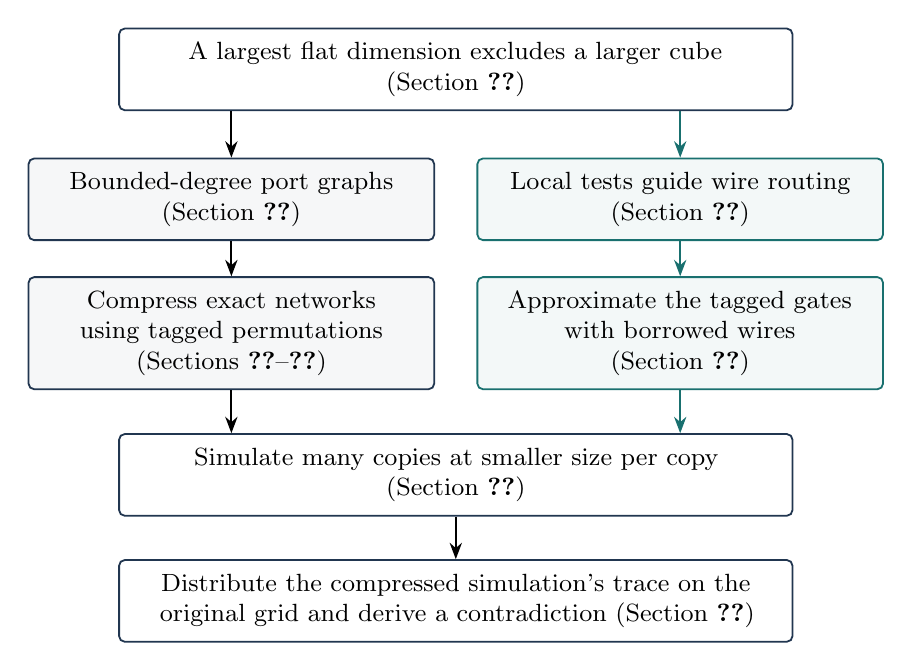
\begin{tikzpicture}[>=Stealth,font=\small,
  box/.style={draw=ink,line width=.65pt,rounded corners=2pt,align=center,
              text width=4.8cm,inner sep=5pt},
  both/.style={box,text width=8.2cm},
  leftbox/.style={box,fill=ink!4},rightbox/.style={box,fill=sea!5,draw=sea},
  flowarrow/.style={->,line width=.65pt}]
\node[both] (cube) {A largest flat dimension excludes a larger cube\\
                     (Section~\ref{sec:prices})};
\node[leftbox] (port) at (-2.85,-1.65) {Bounded-degree port graphs\\
                     (Section~\ref{sec:ports})};
\node[rightbox] (probe) at (2.85,-1.65) {Local tests guide wire routing\\
                     (Section~\ref{sec:protocol})};
\node[leftbox] (comp) at (-2.85,-3.35) {Compress exact networks using tagged permutations\\
                     (Sections~\ref{sec:motifs}--\ref{sec:exact})};
\node[rightbox] (tag) at (2.85,-3.35) {Approximate the tagged gates\\with borrowed wires\\
                     (Section~\ref{sec:width})};
\node[both] (sim) at (0,-5.15) {Simulate many copies at smaller size per copy\\
                     (Section~\ref{sec:descent})};
\node[both] (diag) at (0,-6.75) {Distribute the compressed simulation's trace on the original grid
                     and derive a contradiction (Section~\ref{sec:diagonal})};
\draw[flowarrow] (cube.south -| port.north)--(port.north);
\draw[flowarrow,sea] (cube.south -| probe.north)--(probe.north);
\draw[flowarrow] (port)--(comp);
\draw[flowarrow,sea] (probe)--(tag);
\draw[flowarrow] (comp.south)--(sim.north -| comp.south);
\draw[flowarrow,sea] (tag.south)--(sim.north -| tag.south);
\draw[flowarrow] (sim)--(diag);
\end{tikzpicture}
\caption{The proof by contradiction. The left branch reduces network
size exactly if it may use gates for tagged permutations. The right
branch implements those gates with a controlled error. Compression
also reduces communication when the final argument distributes the
trace of the simulation.}
\label{fig:map}
\end{figure}

\paragraph{Compress exact networks.}
Under cube exclusion, bounded-degree graphs control the mean squared
distance between all pairs of vertices by the mean squared distance
along their edges, for every placement in a spectral space
(Section~\ref{sec:ports}). The construction uses nonlinear spectral
calculus~\cite{MendelNaor,MendelNaorBarycentric,MendelNaorHadamard}.
These \emph{port graphs} restore bounded degree during compression.
A second, fixed wire configuration lets us replace a network by a sum
of networks with fewer bits crossing between groups of vertices.
To assemble that sum into one exact computation, we must keep track of
which tagged records have been routed to which vertices. A
tagged-permutation gate tests that the addresses form a permutation
and that their payloads match. With these gates, the wire replacement
gives an exact reduction in size per copy
(Proposition~\ref{prop:oracle-descent}). Related methods of compressing
wire assignments occur in algorithms for satisfiability
\cite[Appendix~D]{falseeth} and in crossing decompositions~\cite{Anthropic}.

\paragraph{Implement the permutation gates.}
The second use of cube exclusion is local. Place \(k\) pairs of distant
wire endpoints along perpendicular axes at each tested location. If
nearby locations retain the prescribed prices for these wires, their
motion can be read from the changes in distances to the far ends.
A transverse segment in the limit would produce the excluded cube.
These tests range over possible local spectral prices. A failed test
allows a local wire replacement, while
successful tests identify a new link whose effect on subsequent prices
pays for its use. This gives an exact routing identity
(Theorem~\ref{thm:protocol}). Terms that spend too little on links between the layers have low
enough price to discard. Routing the surviving shorter lists recursively gives an approximation for
\(2^h\) records with \(h\)-bit payloads using
\(O(2^h h^{1+\varepsilon})\) trivalent vertices for every fixed
\(\varepsilon>0\) (Theorem~\ref{thm:cheaptag}).

The approximation has an algebraic meaning. Let \(I\) be the tensor
product of wires borrowed in the \(k\) coordinate directions. A
network intended to compute \(f\) while returning those wires produces
a tensor \(X\) in the same spaces as \(f\otimes I\). Its error is the
ordinary difference \(X-f\otimes I\). After fixing the data indices,
it suffices for the simulation that the error have price less than
\(H(I)\) by a specified margin in each prescribed flat placement of
the borrowed wires. The tagged-permutation approximation has this
bound even with its data indices exposed, as required for substitution. The
margin pays for subsequent sums. Once the margin exceeds the premium for adding two errors, a tensor
cannot approximate two distinct scalar multiples of \(I\), since their
difference has the full price \(H(I)\). Inserting these approximate gates into the exact
reduction and reusing borrowed wires along grid lines gives
Theorem~\ref{thm:collapse}. A bounded-degree computation of size \(V\)
with sufficiently few external bits then has an approximation of amortized
size at most \(V/(\log V)^A\) for arbitrarily large fixed \(A\).

\paragraph{Program the contradiction.}
Run many steps of a universal weighted computation on a grid. Let \(Z\)
be its exact tensor and \(\widehat Z\) the tensor obtained by substituting
the smaller simulations. The error estimate gives
\(H(Z-\widehat Z)<H(I)\). At this size, the original grid has enough
capacity to evaluate the accelerated contraction itself, once its trace
has been compressed. Each pair of external wire ends can be routed to
the step that needs its input while the other steps still have their
borrowed wires. We can consequently program the exact contraction to
return \(\widehat Z+I\). Its error is then \(I\), contradicting the
strict price bound. Section~\ref{sec:diagonal} carries out this
diagonal argument, which has a precedent in the use of faster
algorithms to prove circuit lower bounds~\cite{williams}.


\clearpage
{\small\tableofcontents}
\clearpage
\part{The geometry of spectral prices}
\section{The calculus of prices}\label{sec:spectra}
Every spectral point on a fixed set of parties gives a pseudometric on
those parties. The distance between two parties is the logarithm of the
spectral point's value on their binary wire. We first show how the same invariant evaluates tensors on subsets of the
parties and controls the cost of moving their indices. All logarithms are to
base two unless indicated otherwise.

\subsection{Spectral points and prices}
Fix a field $k$ and a finite set $J$ of at least two parties. A tensor has
one finite-dimensional vector space at each party. We use bases throughout,
and contraction is bilinear. Write $X\le Y$ when local linear maps, one at
each party, take $Y$ to $X$. Such a transformation is a \emph{restriction}.
Two operations combine tensors on $J$. In a tensor product we group the
corresponding factors at each party. In a direct sum $X\oplus Y$ we take the
direct sum of the local spaces at every party, so the two summands occupy
separate blocks. Up to mutual restriction, these operations make the tensors
a commutative semiring. Its integer $r$ is the diagonal tensor
\[
                 \Delta_J(r)=\sum_{s=1}^r\bigotimes_{j\in J}e_s.
\]
A nonzero tensor $T$ of rank $R(T)$ satisfies $1\le T\le R(T)$.

A \emph{spectral point} $F$ assigns a nonnegative real number to each tensor.
It preserves $0$ and $1$, is monotone under restriction, and satisfies
\[
       F(X\otimes Y)=F(X)F(Y),\qquad F(X\oplus Y)=F(X)+F(Y).
\]
In particular $F(\Delta_J(r))=r$. Matrix rank after flattening across a
fixed nontrivial cut of $J$ is one example. We call $H(T)=\log_2 F(T)$
the \emph{price} of a nonzero tensor. Tensor products then add prices,
and local maps can only decrease them. The spectral points form a compact
space in the topology of pointwise convergence. Indeed, in standard
coordinate spaces their axioms define a closed subset of the product of
the intervals $[0,R(T)]$.

\subsection{Placement}
For a nonempty $S\subseteq J$, let $\Delta_S(q)$ be the diagonal tensor
sharing a common $q$-valued label among the parties in $S$, with
one-dimensional spaces elsewhere. A singleton diagonal is a nonzero local
vector. For $a\ne b$, the two-party diagonal $E_{ab}(q)=\Delta_{\{a,b\}}(q)$
is a wire of dimension $q$. A wire whose two ends lie at the same party
is also a nonzero local vector. Set
\[
     \delta(S)=H(\Delta_S(2)),\qquad d(a,b)=H(E_{ab}(2)).
\]
Tensoring diagonals multiplies their dimensions, and restriction can
reduce a dimension to any smaller value. Comparing powers of $q$ with
powers of two therefore gives $H(\Delta_S(q))=\delta(S)\log_2 q$.
For a flattening rank, $d(a,b)$ is one when the cut separates $a$ and $b$
and zero otherwise.

For every spectral point, $d$ is a pseudometric. The triangle inequality
comes from joining two wires by contraction at their common endpoint.
A diagonal restricts to a wire between any two of its parties. Conversely,
suppose a tree joins the sites of $S$, possibly through auxiliary vertices.
At each vertex a local map equates its incident wire labels, retaining the
common label at vertices in $S$. Applying these maps to the product of
binary wires produces $\Delta_S(2)$. Hence
\begin{equation}\label{eq:span-price}
 \operatorname{diam}(S)\ \le\ \delta(S)\ \le\
 \sum_{ab\text{ in the tree}} d(a,b).
\end{equation}

A \emph{placement} $x=(x_1,\ldots,x_r)$ assigns the indices of a nonzero
tensor $T$ to parties. We group the indices at each party and write $H(T;x)$ for the
resulting price. Changing a placement keeps the coefficient array of $T$
fixed. To move its $i$th index from $x_i$ to $y_i$, supply a wire of the
index dimension $q_i$ and contract one end with that index at $x_i$.
The same construction moves it back. Thus
\begin{equation}\label{eq:move}
 |H(T;x)-H(T;y)|\ \le\ \sum_{i=1}^r d(x_i,y_i)\log_2 q_i .
\end{equation}
Sites at distance zero may therefore be identified. A nonzero tensor
whose indices are all at one site has price zero.

A \emph{spectral space} is a metric space equipped with prices $H(T;x)$
for all finite placements over $k$. Inserting trivial slots leaves prices
unchanged, and a binary wire has price equal to the distance between its
ends. On each finite set $S$ of positive diameter, all prices must have
the form $\delta(S)\log_2 F_S(T)$ for one spectral point $F_S$ on $S$.
The scale $\delta(S)$ is the price of $\Delta_S(2)$, since
$F_S(\Delta_S(2))=2$. Multiplying all nonzero tensor prices and all
distances by the same positive constant gives another spectral space.
We set $H(0)=-\infty$. Nonzero tensors at a single site and nonzero
scalars on no legs have price zero.

\paragraph{Normalization on subsets.}
Fix a spectral point $F$ on $J$ and a subset $S$ of at least two parties.
Extend tensors on $S$ to $J$ by adjoining trivial slots, and denote the
resulting evaluation by $G$. We have $G(\Delta_S(q))=q^e$ for
$e=\delta(S)$. If $e=0$, the rank bound on $S$ gives $G(T)=1$ for
every nonzero $T$. If $e>0$, the evaluation $G^{1/e}$ is a spectral
point on $S$. Only additivity needs proof, since direct sum on $S$ and
direct sum on $J$ separate blocks at different sets of parties.

Group the terms of $(U\oplus V)^{\otimes n}$ by the number $j$ of
$U$-factors. After local changes of coordinates the $j$th block is
$U^{\otimes j}V^{\otimes(n-j)}\Delta_S(\binom nj)$. Each block is a
restriction of the full tensor. Conversely, the full tensor is the
ordinary sum of the blocks in the ambient spaces. Since an ordinary sum
is a restriction of a direct sum on $J$, $G(U\oplus V)^n$ lies between
the largest block value and $n+1$ times that value. The $1/e$ powers
of the block values are precisely the terms of the binomial expansion
of $(G(U)^{1/e}+G(V)^{1/e})^n$. Their sum lies between the largest
term and $n+1$ times that term. Taking $1/(en)$ powers in the bounds
for $G(U\oplus V)^n$ and letting $n\to\infty$ therefore gives
$G(U\oplus V)^{1/e}=G(U)^{1/e}+G(V)^{1/e}$.

The same normalization works for a list of parties in which several
indices occupy one site. Grouping the indices of a direct sum at that
site introduces additional zero blocks. Deleting those blocks by local
projection gives the direct sum of the grouped tensors, and local
inclusions recover the padded tensor. Equation~\eqref{eq:move} allows
indices at distance zero to move to a common representative without
changing their price. The resulting spectral space on the metric
quotient therefore retains all the original log prices.

\paragraph{Ordinary sums.}
If a product of tensors supplies $T$ by local maps and contractions,
then $H(T)$ is at most the sum of their prices. Suppose instead that
several constructions produce tensors $T_i$ with the same output
spaces on a finite set $S$ of positive diameter. Their auxiliary sites
may differ. Addition in the output spaces is a restriction of a direct
sum on $S$, so the normalized spectral point on $S$ gives
\begin{equation}\label{eq:price-ordinary-sum}
 H\!\left(\sum_i T_i\right)
 \le \delta(S)\log_2\sum_i 2^{H(T_i)/\delta(S)}
 \le \max_i H(T_i)+\delta(S)\log_2\#\{i\}.
\end{equation}
Here $2^{-\infty}=0$. At a single output site every nonzero sum has price
zero. These bounds also apply when terms cancel.

\begin{lemma}[Closure at a fixed placement]\label{lem:spectral-closure}\label{lem:border-test}
In a fixed finite tensor format, if $H(U;x)\le B$ for all nonzero $U$
in a set $\mathcal A$, the same bound holds at every nonzero point of its
Zariski closure.
For geometric closure one takes the tensors and spectral point over an
algebraically closed field \cite[Corollary~2.4]{SpectralSublevels}.
\end{lemma}

\begin{proof}
Write $D$ for the dimension of the ambient tensor space. For every $n$
the map $U\mapsto U^{\otimes n}$ is polynomial. The span of its values
on $\mathcal A$ contains its values on the closure, and has dimension
at most $\binom{n+D-1}{D-1}$ by expanding in monomials in the coordinates
of $U$. Thus for $T$ in the closure, $T^{\otimes n}$ is an ordinary sum of
at most that many scalar multiples of powers from $\mathcal A$.
Apply \eqref{eq:price-ordinary-sum} at the placement $x$ and divide by $n$.
The error tends to zero with the format and placement fixed.
\end{proof}

\subsection{Limits of spectral spaces}\label{sec:limits}
Two limiting operations preserve these data. For metric completion take
the limit of every fixed tensor price along convergent placements,
using \eqref{eq:move}. For a pointed metric ultralimit, possibly after
rescaling, take the ultralimit of prices of the representing placements.
For each fixed nonzero tensor these numbers are bounded by \eqref{eq:move}
because its indices are a bounded distance from the basepoint.
The same bound gives independence of representatives and agreement when
two parties merge. On a finite limit set of positive diameter, the
multipliers $\delta(S)$ are bounded above and away from zero by
\eqref{eq:span-price}. Dividing by them and passing to the limit preserves
all spectral point axioms. Thus the limits carry simultaneous values
for every tensor, including tensors over uncountable fields.


\subsection{Turning prices into restrictions}
Monotonicity gives a necessary condition for a tensor restriction.
A strict inequality at every spectral point has a converse for powers
of the tensors. We use the following form of Strassen's asymptotic
spectral theory \cite{Strassen1988} (see also \cite{Fritz,WZ}).
\begin{lemma}[Strict spectral comparison]\label{lem:spectral-comparison}
Suppose that $X,Y$ are nonzero and $F(X)<F(Y)$ for every spectral
point on $J$. There is an integer $K\ge 1$ such that
$K Y^m\ge X^m$ for every $m\ge 1$.
\end{lemma}
\begin{proof}
The proof separates an element from the cone of restrictions by a
spectral point, then clears the denominators in the resulting cone
inequality. Pass to the additive group completion of the tensor semiring
$S_J$ and localize at all
nonzero tensors, obtaining a commutative $\mathbb Q$-algebra
$A$. Nonzero tensors form a multiplicative set, and flattening rank
extends to this localization. Let $P$ be the cone of finite sums of
$(a-b)/s$ with $a\ge b$ and $s$ a nonzero tensor. This rational
convex cone is closed under multiplication by tensor fractions $t/s$.
Write $v\le_P w$ if $w-v\in P$. Every element of $A$ is between
integer bounds in this order, since $0\le_P t/s\le_P t$.
Evaluating at a flattening rank shows that $-1\notin P$.

We claim that $z\notin P$ implies the existence of a spectral point
whose extension to $A$ takes a nonpositive value at $z$. Indeed,
$P'=P-\mathbb Q_{\ge0}z$ also excludes $-1$, since $-1=p-qz$
with $p\in P$ would give $q>0$ and $z=(1+p)/q\in P$.
Extend the identity on $\mathbb Q1$ to a rational-linear functional
on $A$ positive on $P'$ (where positive means nonnegative on the
cone). For the extension by a new direction $h$, prescribe a value
between the supremum on old vectors bounded above by $h$ and the
infimum on old vectors bounded below by $h$, using the order of $P'$.
Integer bounds make the two sets nonempty, positivity orders their
values, and rational rescaling verifies the extension. Well-ordering $A$
gives the functional, with value at $z$ at most zero.

The rational-linear functionals positive on $P$ with value one at the
unit form a compact convex set, by the integer bounds. Minimize
evaluation at $z$, then (taking intersections at limit stages) minimize successively on a well-ordered list of
all coordinates in the preceding minimizing faces. The nested compact
faces have a unique common member $\ell$, which is extreme and has
$\ell(z)\le0$. For any nonzero tensor $s$, put $u=s/(1+s)$ and
$v=1/(1+s)$. Multiplication by either preserves $P$, and $u+v=1$.
If $s\le r$, both $u,v$ are at least $1/(r+1)$ in the cone order,
using $s\ge1$. Thus the functionals $\ell(u\,\cdot)$ and
$\ell(v\,\cdot)$ normalize to states and decompose $\ell$ with
positive coefficients. Extremality gives
$\ell(uh)=\ell(u)\ell(h)$ and $\ell(vh)=\ell(v)\ell(h)$.
As $vs=u$, it follows that $\ell(sh)=\ell(s)\ell(h)$.
The restriction of $\ell$ to tensors is the desired spectral point,
and the same identity determines its extension to fractions.

By compactness choose an integer $b$ with
$b F(Y)>(b+1)F(X)$ at every spectral point. The claim gives
$bY-(b+1)X\in P$. Collecting denominators and clearing the
localization gives $cbY-c(b+1)X=a-a'$ in the additive group
completion, for some nonzero tensor $c$ and tensors $a\ge a'$.
Equality in the completion allows addition of a common tensor in
$S_J$, so $cbY+w\ge c(b+1)X+w$ for some $w$ (absorb $a'$ into
$w$). Choose $q$ with $qcY\ge w$, possible since $cY\ge1$.
Trading $q$ times while retaining $w$ gives
\[
 q(b+1)cY\ \ge\ qbcY+w\ \ge\ q(b+1)cX+w\ \ge\ q(b+1)cX .
\]
Consequently $c'Y\ge c'X$ with $c'=q(b+1)c$. Reusing $c'$ gives
$c'Y^m\ge c'X^m$ for every $m$. Any integer $K\ge c'$ works.
\end{proof}


Strict comparison also lets us change the ground field without losing
prescribed spectral values (see \cite{Strassen1988,CVZ}).
\begin{lemma}\label{lem:comparison}
For $k\subseteq K$, the possible joint values of spectral points on
any family of tensors defined over $k$ are the same over the two fields.
\end{lemma}

\begin{proof}
Restricting spectral points over $K$ to tensors over $k$ gives a compact
subset of the spectrum over $k$. If this subset misses $F$, there are
finitely many tensor evaluations whose values at $F$ do not occur
jointly in the subset. Choose a rational polynomial in those evaluations
which is negative at $F$ and positive on the compact image. For example,
approximate the squared distance to the tuple at $F$, minus a small
positive constant. After clearing denominators, the polynomial is the
difference in evaluation of two nonzero tensors $Y,X$. Monomials
correspond to tensor products, and adding $1$ to both parts ensures
that $X$ and $Y$ are nonzero.

By Lemma~\ref{lem:spectral-comparison} over $K$ there is a fixed integer
$C$ such that $X^m\le C Y^m$ for all $m$. Fix $m$. The finitely many
coefficients of the local maps generate a $k$-algebra. Taking its
quotient by a maximal ideal specializes the restriction to a finite
extension $L/k$ by Zariski's lemma. The $n$th power of this restriction
is still given by one linear map per party over $L$. Expand each map
in a $k$-basis of $L$ and apply a $k$-linear functional $L\to k$ that
takes $1$ to $1$. This expresses $X^{mn}$ over $k$ as an ordinary sum
of at most $[L:k]^{|J|}$ scaled restrictions of $(CY^m)^n$. Hence
\[
              F(X)^{mn}\le [L:k]^{|J|} C^nF(Y)^{mn}.
\]
Taking $n$th roots and letting $n\to\infty$ gives
$F(X)^m\le C F(Y)^m$. Since $C$ is independent of $m$, this contradicts
$F(X)>F(Y)$.
\end{proof}
\section{Geodesic extension}
\label{sec:geodesic}
Can one insert a point between two existing sites while preserving the
prices of all tensors on the old sites? The next theorem gives such an
extension for every division of the distance between the sites. Its
second assertion adds a site at the center of a star and identifies the
least possible weighted sum of the new wire lengths. We then use an
exterior-algebra identity to control tensor prices as one or more
indices move between sites.
\subsection{Extending a spectral point by one party}

For an additional party $p$, let $\iota$ embed old tensors by the
trivial leg at $p$. We say $F'$ \emph{extends} $F$ if
$F'(\iota T)=F(T)$ for every old tensor. This condition fixes the
old spectrum values, including those of tensors with many
nontrivial legs.

\begin{theorem}[Exact extension]\label{thm:extension}
Let $F$ be a spectral point on $J$ over $k$, and write
$d_F(a,b)=\log_2 F(E_{ab}(2))$.
\begin{enumerate}
\item For $a\ne b$ in $J$ and any nonnegative $\lambda_a,\lambda_b$ with
$\lambda_a+\lambda_b=d_F(a,b)$ there is an extension by $p$ such
that $d_{F'}(a,p)=\lambda_a$ and $d_{F'}(p,b)=\lambda_b$.
\item For integers $w_i\ge 0$ on $J$, put
\[
 g_F(w)=\sup_{h\ge1,\ T\ne0}
                  \frac{\log_2 F(T)}h ,
 \qquad T\in\bigotimes_{i\in J} k^{2^{hw_i}},
 \quad h\in\mathbb Z.
\]
Then
\begin{equation}\label{eq:spectral-star}
                 g_F(w)=\min_{F'\text{ extends }F}
                             \sum_{i\in J} w_i d_{F'}(p,i).
\end{equation}
For each width profile $w$ the minimum is attained by an extension
whose center $p$ may depend on $w$. Taking $w$ to be the indicator
of a subset gives the equal-dimension star.
\end{enumerate}
\end{theorem}
\begin{proof}
Use the embedded nonzero old tensors as generators with prescribed
targets $f(\iota T)=F(T)$. For the first assertion add generators
$E_{pa}(2),E_{pb}(2)$ with targets $2^{\lambda_a},2^{\lambda_b}$.
For the second add the single generator
$S_w=\prod_i E_{pi}(2^{w_i})$ with target $2^{g_F(w)}$.
The rank bound gives $0\le g_F(w)\le\sum_i w_i$.
Targets multiply on formal monomials in the selected generators.

Contract the new leg of such a monomial $M$ by a covector. The old
spectral value of the result is at most $f(M)$. The old factors pass
unchanged through the contraction. In the first case the remaining
tensor is a matrix of rank at most $2^{\min(u,v)}$, where $u,v$ are
the respective wire multiplicities. Its value is at most
$2^{d_F(a,b)\min(u,v)}\le 2^{u\lambda_a+v\lambda_b}$.
In the second case a covector on the center of $S_w^u$ gives exactly
an arbitrary tensor of dimensions $2^{uw_i}$, whence the bound.
This also shows $g_F(w)\le\sum_i w_i d_{F'}(p,i)$ for every
extending $F'$.

Let $C_m$ be the supremum of the old spectral values of contractions of
$M^m$ at $p$. In the first case with $u=v$, choosing the identity
matrix gives $C_m=f(M)^m$. In the star case write
$M=(\iota T_0)S_w^u$, combining the embedded old factors into $T_0$.
Fix $h\ge1$ and a nonzero tensor $T$ of local dimensions $2^{hw_i}$.
For every $m$, take $\lfloor um/h\rfloor$ copies of $T$ and pad the
remaining dimensions by a nonzero simple tensor. The result is a
contraction of $S_w^{um}$, so
\[
  F(T_0)^m F(T)^{\lfloor um/h\rfloor}\le C_m\le f(M)^m .
\]
Taking the lower limit of $m$th roots gives
$\liminf_m C_m^{1/m}\ge F(T_0)F(T)^{u/h}$. Taking the supremum over
$h,T$ gives $C_m^{1/m}\to f(M)$, including when $u=0$.

We have bounded the spectral value of every contraction by its monomial
target. The bound is sharp in exponential rate for a monomial with balanced
wire multiplicities in the first case and for every star monomial in the
second. We now use strict spectral comparison to show that the targets
are attained simultaneously.
Suppose no spectral point attains them all. Compactness then gives a finite list $G_1,\ldots,G_s$, including
the added generators, and $\delta>0$ such that every spectral point
$F'$ on $J\cup\{p\}$ has some ratio $F'(G_i)/f(G_i)$ or its inverse
at least $1+\delta$. Let $M=\prod_i G_i^e$ and let
$M_1,\ldots,M_{2s}$ be the variants obtained by changing exactly one
exponent either from $e$ to $0$ or from $e$ to $2e$. Take $e$ large
enough that $(1+\delta)^e>8s$. Choose positive integers $L,c_j$ by
rational approximation so that
\[
 \frac1{8s}<\frac{c_j f(M_j)}{L f(M)}<\frac1{4s}
 \qquad(1\le j\le 2s).
\]
For any $F'$, the violating index and the choice of sign give an
index $j$ with $c_jF'(M_j)>L F'(M)$. By
Lemma~\ref{lem:spectral-comparison} there is a fixed $K$ with
\[
 (L M)^m\ \le\ K\biggl(\bigoplus_{j=1}^{2s} c_jM_j\biggr)^m
 \qquad(m\ge1).
\]
On the left apply at $p$ the all-ones covector on the $L^m$-copy
factor, times a covector on $M^m$ whose contraction has old spectral
value greater than $C_m/2$. Such a covector exists since $0<C_m<\infty$. The
copy factor becomes the full $L^m$-fold diagonal on the old parties.
The equal multiplicities required in the first case hold for $M$.
The resulting old values therefore approach $L f(M)$ after taking
$m$th roots. On the right, pull the covector back through the restriction at
$p$ and restrict it to each direct-sum branch. On a branch the input
is a monomial $(\iota T_*)V$, with $T_*$ the product of its old
tensors. Its leg at $p$ is just that of $V$, so an arbitrary covector
$\xi$ there gives the old tensor $T_*\,\xi(V)$ before applying the
old-party maps. Those maps commute with contraction at $p$ and can
only decrease the value. The contraction bound above applies jointly
to $V$, using its total wire multiplicities. A star power gives a
single tensor of the prescribed local dimensions and the split wires
give a single matrix of bounded rank. Thus each branch is bounded by
its monomial target without a factorization assumption on $\xi$.
Summing over branches by ordinary subadditivity bounds the old value by
$K(\sum_j c_j f(M_j))^m$. Since $\sum_j c_j f(M_j)<L f(M)/2$,
this is impossible for large $m$. The spectral point matching the
targets proves both assertions.
\end{proof}

Theorem~\ref{thm:extension} extends to arbitrary spectral spaces.
Apply the finite theorem, with the appropriate scale, on each finite
subset containing the specified sites. For the star give weight zero
to any additional sites and use prices in place of log spectral
values. Take the pointed ultralimit from Section~\ref{sec:limits}
along an ultrafilter containing all tails of this directed family.
Take a specified site as basepoint, choosing one of positive weight
for a star. The prescribed distance or the bound on the star sum keeps
the new point at bounded distance from the basepoint. The limit therefore
contains the new point and preserves every old price. Repeated sites
in a star are handled by adding their weights. For zero weights
throughout, or a singleton space, any old site serves as center.
\subsection{Relocating one tensor index}

To interpolate the price of a tensor, we first move a single index.
On an auxiliary exterior algebra, the sum of two operator products
in opposite orders recovers the original tensor index. Related fermionic constructions occur in
the crossing identity \cite{Anthropic,Khoruzhii} used in
Section~\ref{sec:crossing}.
Fix a spectral point $F$ and write $d=d_F$. Consider a tensor with a
specified local factor $k^q$. Write $T_A$ for its coefficient array
with that factor placed at $A$ and every other factor in its original
position. Moving the factor from $B$ to $A$ is a restriction after
supplying a $q$-dimensional wire between $A$ and $B$. Consequently
\[
                         F(T_A)\le q^{d(A,B)}F(T_B).
\]
Two indices of a wire at the same party give a nonzero local vector,
equivalent by restriction to the unit, even if the characteristic
divides $q$. Thus the estimate holds also for repeated parties, and
moving a factor a distance zero preserves its value.

On the exterior algebra $\bigwedge k^Q$, for integers $Q\ge2$, write
$L_i$ for left exterior multiplication by the $i$th basis vector
and $D_j$ for contraction by the $j$th dual basis vector. Explicitly,
\[
 D_j(v_1\wedge\cdots\wedge v_b)
   =\sum_{a=1}^b(-1)^{a-1}(v_a)_j\,
      v_1\wedge\cdots\wedge\widehat{v_a}\wedge\cdots\wedge v_b .
\]
In particular $D_j(e_i\wedge v)=\delta_{ij}v-e_i\wedge D_jv$, or
\begin{equation}\label{eq:wire-exterior}
                       D_j L_i+L_i D_j=\delta_{ij}I .
\end{equation}
This identity holds over the integers in the ordered subset basis, so
also in characteristic two. On $\bigwedge^b k^Q$ write
$R=\binom Qb$ and $R_\pm=\binom Q{b\pm1}$. For each fixed
$s\in[-1,1]$ we may take $1\le b\le Q-1$ so that, as $Q\to\infty$,
\begin{equation}\label{eq:wire-binomial}
                   R_+/R=Q^{s+o(1)},\qquad R_-/R=Q^{-s+o(1)} .
\end{equation}
For $s>0$ use $b=\lfloor Q^{1-s}\rfloor$ for sufficiently large
$Q$, for $s<0$ take the complementary level for $-s$, and for $s=0$
use a middle level. The ratios are $(Q-b)/(b+1)$ and $b/(Q-b+1)$.

\begin{lemma}[One index]\label{lem:wire-one-index}
Let $0\le u\le1$ and suppose $d(A,C)=u\,d(A,B)$ and
$d(C,B)=(1-u)d(A,B)$. Every nonzero tensor with a marked index
satisfies $F(T_C)\le F(T_A)^{1-u}F(T_B)^u$.
\end{lemma}
\begin{proof}
Put $t=d(A,B)$. The index-moving estimate handles $t=0$ and
$u\in\{0,1\}$. A one-dimensional index is trivial, so assume $q\ge2$
and $0<u<1$. In the $n$th power the marked index has dimension $Q=q^n$.
Using the matrices in Equation~\eqref{eq:wire-exterior}, replace the
marked index $j$ by a fresh index $i$ of the same dimension, with row
and column indices $\beta,\alpha$ on $\bigwedge^b k^Q$ at $B,A$.
The two arrays have entries
\[
   \sum_j(D_jL_i)_{\beta\alpha}(T^n)_{\ldots j\ldots}
   \quad\text{and}\quad
   \sum_j(L_iD_j)_{\beta\alpha}(T^n)_{\ldots j\ldots}.
\]
Their sum, with $i$ at $C$, is $T_C^n E_{AB}(R)$.
The two arrays have local implementations with the following wire
dimensions. In both rows $\alpha$ starts at $A$, $\beta$ ends at $B$,
and the new index $i$ is at $C$.
\[
\begin{array}{ccccc}
 A && C && B\\[2pt]
 \alpha & \xrightarrow{\ R\ } & L_i & \xrightarrow{\ R_+\ } & D_j\\[2pt]
 D_j & \xrightarrow{\ R_-\ } & L_i & \xrightarrow{\ R\ } & \beta
\end{array}
\]
Contraction by $D_j$ uses the old index of $T_B^n$ in the first row
and that of $T_A^n$ in the second. Both implementations are local
restrictions even when sites coincide. Subadditivity, $d(A,C)=ut$ and $d(C,B)=(1-u)t$
give
\[
 F(T_C)^n\le F(T_B)^n(R_+/R)^{(1-u)t}
                    +F(T_A)^n(R_-/R)^{ut}.
\]
Set $s=t^{-1}\log_q(F(T_A)/F(T_B))$, which lies in $[-1,1]$ by the
index-moving estimate. Use Equation~\eqref{eq:wire-binomial} and take
$n$th roots. The two candidate limits for the maximum are
$F(T_B)q^{(1-u)ts}$ and $F(T_A)q^{-uts}$, both equal to
$F(T_A)^{1-u}F(T_B)^u$.
\end{proof}

\subsection{Moving several indices together}
Consider a binary wire whose ends both move from $a$ to $b$ and occupy
the same site at fraction $t$ of the journey. Its price there is zero.
Interpolating one end at a time compares its price with the average
for two independent endpoint choices, namely $2t(1-t)d(a,b)$. Choosing
the same endpoint for both ends gives the sharp bound zero. Such
synchronized choices are available for every tensor. More generally,
the endpoint choices can have any joint law with the prescribed marginals.
\begin{proposition}[Joint convexity of placement]\label{prop:joint-convexity}
For each marked index $i$ let $z_i$ have distances
$t_i d_i,(1-t_i)d_i$ to $a_i,b_i$, respectively, where
$d_i=d(a_i,b_i)$ and $0\le t_i\le1$. For any probability law $\mu$
on endpoint choices choosing $b_i$ with probability $t_i$
and $a_i$ otherwise, with $x_i$ the chosen position,
\[
                 H(T;z)\le \mathbb E_\mu H(T;x).
\]
Unmarked indices keep their positions.
\end{proposition}

\begin{proof}
The assertion is immediate for $T=0$ or if every move is constant.
Omit constant moves and one-dimensional marks, and normalize prices by
the scale on the finite set of all positions. Successive applications
of Lemma~\ref{lem:wire-one-index} give the bound when the endpoint
choices are independent. Under any coupling with the same marginals,
a function of the form $c_0+\sum_i f_i(x_i)$ has the same expectation.
We use the exterior identity to decompose $T^{\otimes n}$ into terms
whose bounds at the endpoints approach functions of this form.

Divide log prices by $n$. Each term has the original marked positions
and some auxiliary indices at fixed sites. We record an upper bound
$N(x)$ for its normalized price at each endpoint configuration $x$,
after subtracting the normalized prices of the auxiliary wires adjoined
along its branch. These bounds may have an error $o(1)$ as $n\to\infty$.
The initial table for $T^{\otimes n}$ is $N(x)=H(T;x)$.

Choose one mark of original dimension $q$, with endpoints $a,b$ at
distance $d>0$. Its current dimension is $Q=q^n$. On exterior
degree $l$ of $k^Q$, multiplication by a basis vector $i$ and
contraction by the dual vector $j$ satisfy
\[
                 D_jL_i+L_iD_j=\mathbf 1_{i=j} I .
\]
Adjoin the $ab$-wire of dimension $R=\binom Ql$. Use this identity on
it, summing against the old index $j$ and leaving the new index $i$
marked. The two terms form two child nodes. At either endpoint a child
can be made using both operators there and the $R$-wire. In the first
term, with the new index at $a$, one may instead put creation at $a$
and the old index with contraction at $b$, using a wire of dimension
$R_+=\binom Q{l+1}$. In the second term the reversed placement uses
$R_-=\binom Q{l-1}$ between the operators.

Write $N_0,N_1$ for the two slices at $a,b$. For any
$|c|\le d\log_2 q$ choose $l$ so that
$(d/n)\log_2(R_\pm/R)=\pm c+o(1)$. For $s=c/(d\log_2 q)>0$ take
$l=\lfloor Q^{1-s}\rfloor$, for $s<0$ take the complementary level
for $-s$, and for $s=0$ take a middle level. After subtracting the
price of the adjoined wire the child tables may therefore be taken as
\[
 \bigl(\min\{N_0,N_1+c\},N_1\bigr),\qquad
 \bigl(N_0,\min\{N_1,N_0-c\}\bigr),
\]
with entrywise minima. The passage from $N_1$ to $N_1+c$, for instance, is precisely the alternative $R_+$ implementation at $a$.
A zero child may be discarded.
Choose $c$ midway between the extreme entries of $N_0-N_1$. Writing $D=N_0-N_1$, the new differences are $\min(D,c)$ and
$\max(D,c)$. Thus the range of differences starts in
$[-d\log_2 q,d\log_2 q]$ by \eqref{eq:move}, and each split reduces
its width by at least half. The bounds on differences along every other
coordinate are preserved, since entrywise minimum is monotone and
commutes with addition of a constant.

After sufficiently many rounds with every mark, the variation of each
coordinate difference in any leaf table is at most $\epsilon$.
Consequently each such table with $r$ marks lies within $r\epsilon$
of a function of the form $c_0+\sum_i f_i(x_i)$, by telescoping
coordinate changes from one corner. The means of this latter function
under the product law and $\mu$ agree. Apply independent relocation to
the leaf tensor, with auxiliary indices fixed, and subtract the accumulated
wire prices. Its price is bounded by the $\mu$-mean of its table plus
$2r\epsilon+o(1)$, hence by the same expression using the original table,
as entries only decreased. At each split the new wire's price cancels
and ordinary subadditivity costs at most $1/n$ in the normalized log.
For fixed $\epsilon$ the depth is fixed. Let $n\to\infty$ and then
$\epsilon\downarrow0$.
\end{proof}


Write $[a,b]_t$ for a point at distances $t\,d(a,b)$ from $a$ and
$(1-t)d(a,b)$ from $b$.
\begin{corollary}[Geodesic extension]\label{cor:spectral-geodesic}
Every spectral space embeds with prices unchanged into a complete uniquely geodesic spectral space.
Prices are convex along simultaneous geodesics. In particular in any spectral space,
if the two interval points exist,
\begin{equation}\label{eq:wire-busemann}
 d([a,b]_t,[c,e]_t)\le (1-t)d(a,c)+t d(b,e)
                       \qquad (0\le t\le1).
\end{equation}
\end{corollary}
\begin{proof}
Apply Proposition~\ref{prop:joint-convexity} to the ends of a binary
wire with the same endpoint choice for both ends. At a common fraction
$t$ the distance between interval points is bounded by
$(1-t)d(a,a')+t d(b,b')$ for their endpoint pairs $(a,b),(a',b')$.
This implies uniqueness of each interval point. Use
Theorem~\ref{thm:extension} and its infinite-space version to insert midpoints for all pairs, taking
successive extensions and their union for an infinite set of pairs.
Repeat in countably many rounds, then take the completion. The midpoint
estimate extends midpoints to the completion, and iterated bisection
gives constant-speed segments. Propagating prices through these steps as
above gives a complete geodesic spectral space $X$. On such a space
the synchronized endpoint choice in Proposition~\ref{prop:joint-convexity}
gives convexity of every price along simultaneous geodesics.
\end{proof}

\section{From crossing decompositions to nonpositive curvature}
\label{sec:crossing}

The geodesic extension of Section~\ref{sec:geodesic} gives convexity of
wire distances. To obtain nonpositive curvature, we need a quadratic
bound on those distances. Its algebraic source is a decomposition of two
wires into two tensors that factor across different cuts of the four
endpoints. The cost of the internal wire on one cut can be traded
against its cost on the other. We use this tradeoff first to prove the
parallelogram law for normed planes realized by wire distances and then
to prove the squared midpoint inequality in every geodesic spectral
space.

\subsection{The integral crossing identity}\label{app:crossing}

The crossing construction originates in work of Anthropic~\cite{Anthropic}.
Khoruzhii~\cite{Khoruzhii} gives an integral construction in which two
products of fermionic operators factor through states below the same
energy bound. Extracting a shifted coefficient changes the two bounds
by equal and opposite amounts.
\begin{theorem}[Shifted crossing]\label{thm:crossing}
Let $t,u>0$, put $S=t^2+u^2$, and take $-S<\delta<S$. There are
integers $d_X,d_Y$, depending on $n$, with
$\log_2 d_X=nt+o(n)$ and $\log_2 d_Y=nu+o(n)$, for which the
two-wire tensor has the ordinary sum decomposition
\[
 E_{X_+X_-}(d_X)\,E_{Y_+Y_-}(d_Y)=T_++T_-.
\]
On the cuts $X_+Y_+\mid X_-Y_-$ and $X_+Y_-\mid X_-Y_+$ respectively,
$T_+$ and $T_-$ have flattening ranks at most
\[
  2^{n\sqrt{S+\delta}+o(n)}
  \quad\text{and}\quad
  2^{n\sqrt{S-\delta}+o(n)} .
\]
One can choose the tensors and their two matrix factorizations over
$\mathbb Z$, so the same choices work over every field.
\end{theorem}

The two terminal pairs $(X_+,X_-)$ and $(Y_+,Y_-)$ carry the original
wires. Each summand can be represented by joining two local factors
with a single internal wire, as in Figure~\ref{fig:crossing-cuts}.
In the integral construction, the internal wire records the intermediate
state of a product of operators together with auxiliary summation indices.
There are polynomially many choices of the auxiliary indices at the given
energy cutoff. Reversing the order of the operators exchanges the two cuts. The shift $\delta$ lets us choose how much dimension to
allow on each internal wire.

\begin{figure}[htbp]
\centering
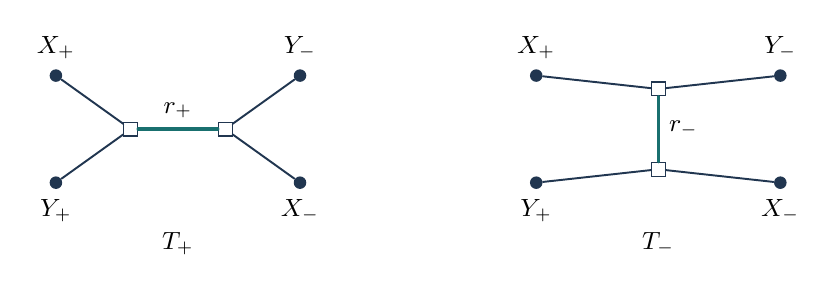
\begin{tikzpicture}[x=1cm,y=1cm,line cap=round,
    terminal/.style={circle,fill=ink,inner sep=1.6pt},
    factor/.style={rectangle,draw=ink,fill=white,inner sep=2.5pt},
    wire/.style={line width=.7pt,draw=ink},
    internal/.style={line width=1.2pt,draw=sea},font=\small]
\foreach \a in {0,6.1}{
  \begin{scope}[xshift=\a cm]
    \node[terminal,label=above:$X_+$] (xp) at (-1.55,.68) {};
    \node[terminal,label=above:$Y_-$] (ym) at (1.55,.68) {};
    \node[terminal,label=below:$Y_+$] (yp) at (-1.55,-.68) {};
    \node[terminal,label=below:$X_-$] (xm) at (1.55,-.68) {};
    \ifdim\a pt=0pt
      \node[factor] (a) at (-.60,0) {};
      \node[factor] (b) at (.60,0) {};
      \draw[wire] (xp)--(a)--(yp) (ym)--(b)--(xm);
      \draw[internal] (a)--node[above] {$r_+$} (b);
      \node at (0,-1.45) {$T_+$};
    \else
      \node[factor] (a) at (0,.51) {};
      \node[factor] (b) at (0,-.51) {};
      \draw[wire] (xp)--(a)--(ym) (yp)--(b)--(xm);
      \draw[internal] (a)--node[right] {$r_-$} (b);
      \node at (0,-1.45) {$T_-$};
    \fi
  \end{scope}
}
\end{tikzpicture}
\caption{The two factorizations of Theorem~\ref{thm:crossing}.
In each summand the two squares are local tensors. The wire joining
them has dimension equal to the flattening rank $r_+$ or $r_-$ across
the corresponding cut. The dimensions on the four outer wires agree in
both summands.}\label{fig:crossing-cuts}
\end{figure}

\begin{proof}[Proof of Theorem~\ref{thm:crossing}]
The construction has three steps. We identify an integral pairing
of operators, factor it through states with two different energy
bounds, and count the states allowed by each bound.

\smallskip\noindent\emph{The pairing.}
Use the exterior algebra over $\mathbb Z$ on generators indexed by
$i\ge 0$. Its basis states are finite subsets of these indices,
written in increasing order. Let $c_i$ wedge the $i$th generator on
the left and let $a_i$ be its signed deletion. Creation operators
anticommute with one another, as do deletion operators, and
$a_i c_j+c_j a_i=\mathbf 1_{i=j}\mathrm{Id}$. Give a basis state $I$
energy $h(I)=\sum_{i\in I}(i+1/2)$. For background on the free fermion and vertex superalgebras see \cite{KacWang}. Introduce the fields
\[
 \psi(z)=\sum_{i\ge0}(c_i z^i+a_i z^{-i-1}),
 \qquad \psi_j(z)=\partial^{(j)}_z\psi(z),
 \qquad Y_I(z)={:}\prod_{i\in I}\psi_i(z){:}.
\]
Here $\partial^{(j)}_z z^b=\binom bj z^{b-j}$ for every integer $b$,
using the coefficient of $v^j$ in $(z+v)^b$. The product is ordered
by increasing $i$. The colons instruct us to expand and move creations
to the left of deletions using permutation signs only. Such a normal
product is skew under interchange of two fields. A coefficient $[z^b]Y_I$
shifts energy by $b+h(I)$. Indeed each summand of a differentiated
field shifts energy by its exponent plus the index of differentiation
plus $1/2$.

For equally large nonempty sets $I,J$, put $m=|I|=|J|$, $h=h(I)$,
$h'=h(J)$ and $L=h+h'-1$, a nonnegative integer. We claim
\begin{multline}\label{eq:crossing-field}
 (z-w)^L\big(Y_I(z)Y_J(w)-(-1)^{m^2}Y_J(w)Y_I(z)\big)
   \\= C_{IJ}\sum_{s\in\mathbb Z}z^{-s-1}w^s\,\mathrm{Id},
\end{multline}
where
\[
 C_{IJ}=(-1)^{\binom m2+\sum_{i\in I}i}
       \det\left[\binom{i+j}{i}\right]_{i\in I,\,j\in J}.
\]
To see this, normal order the product of the two blocks. When a
deletion from the first block meets a creation from the second, the
anticommutation relation permits either a signed interchange or a
scalar contraction. Summing the scalar for fields $i,j$ gives the
expansion in $w/z$ of
\[
  \partial^{(i)}_z\partial^{(j)}_w\frac{1}{z-w}
   =\frac{(-1)^i\binom{i+j}{i}}{(z-w)^{i+j+1}},
\]
since the undifferentiated contraction is
$\sum_{r\ge0}z^{-r-1}w^r$. Thus the expansion is indexed by partial
matchings between the blocks. Each summand is the product of the
matched scalars times the normal product of the unmatched fields.
Its sign is that of the permutation listing the matched pairs first,
in first-field/second-field order within each pair, followed by the
unmatched fields in their original order. In fact the sign for a
contraction is the sign of bringing the two operators together.
Moving the resulting pair as a block incurs no further sign.

For the reversed product, use the same ordering of pairs and the
same final order of the unmatched fields. Interchanging the original
blocks contributes $(-1)^{m^2}$. Reversing the orientation of any
pair contributes a further minus sign in the permutation, precisely
canceled by reversing its rational kernel, since
$(-1)^j/(w-z)^{i+j+1}=(-1)^{i+1}/(z-w)^{i+j+1}$. Consequently after
multiplication by $(-1)^{m^2}$ the reversed summands expand the same
rational kernels in $z/w$. For an incomplete matching an unmatched
field in each block accounts for at least one unit of missing pole
order. Its pole order is therefore at most $L$, and multiplication
by $(z-w)^L$ makes the two expansions equal. For a full matching the
pole order is $L+1$. Interleaving the two increasing lists contributes
$(-1)^{\binom m2}$, permuting partners contributes the determinant
sign, and the kernels contribute the remaining row signs in $C_{IJ}$.
The two expansions of $1/(z-w)$ differ by
$\sum_{s\in\mathbb Z}z^{-s-1}w^s$. This proves
\eqref{eq:crossing-field}.

We justify the formal products coefficientwise. Truncate the modes at
$N$ and first
perform the two normal-ordering expansions with their truncated scalar
kernels. Fix input and output states and a monomial $z^b w^{b'}$.
In the first product the intermediate energy is the input energy plus
$b'+h'$. In the reversed product the increment is $b+h$. There are
only finitely many states at either energy. Each individual normal
block between specified states uses deletion modes from its input
and creation modes from its output. Hence its matrix coefficient
stabilizes as a Laurent polynomial. The same argument applies to
the unmatched normal product, even in two variables. For each of its
finitely many monomials, prescribing the total $w$-power bounds all
contracted modes in the first expansion: a creation in mode $r$
differentiated $j$ times has $w$-power $r-j\ge0$ whenever its
coefficient is nonzero. The reversed expansion uses the $z$-power in
the same way. Both Wick expansions therefore pass coefficientwise to
the infinite-mode limit, where the rational-kernel cancellation above
applies. Multiplication by the fixed polynomial $(z-w)^L$ preserves
these limits. All coefficients are integers, including the divided
derivatives, so reduction modulo $2$ also preserves the identity.

\smallskip\noindent\emph{The factorizations.}
Let $D(H)$ count the states of energy at most $H$, with $D(H)=0$ for
$H<0$. Fix $H,E\ge1$ and an integer $s$. Use nonempty $I,J$ of
energy at most $H$, and input and output states $\beta,\alpha$ of
energy at most $E$. For a block of given $m,h,h'$ take
$[z^{-s-1}w^s]$ in \eqref{eq:crossing-field}. For the multiplier
monomial $z^{L-a}w^a$, $0\le a\le L$, the first product acts on
$\beta$ first by $[w^{s-a}]Y_J$, reaching energy at most
$E+h'+s-a\le E+H+s$. The reversed product acts first by
$[z^{-s-1-L+a}]Y_I$, reaching energy at most
$E-s-h'+a\le E+H-s$. Sum over intermediate states in each matrix
product. This writes $C_{IJ}\mathbf 1_{\alpha=\beta}$ as a sum of
two matrices, each factored over $\mathbb Z$. On the cut
$(I,\alpha)\mid(J,\beta)$ the first factors through at most
$(L+1)D(E+H+s)$ coordinates, indexed by $a$ and the intermediate
state. On the cut $(I,\beta)\mid(J,\alpha)$ the second factors
through at most $(L+1)D(E+H-s)$ coordinates. The integer coefficients
of the multiplier and the sign of the reversed product can be placed
on either factor.

Extend each block by zero and sum over $m,h,h'$. The number of blocks
and the largest $L+1$ are bounded by a polynomial in $H+1$, since
all energies are half-integers and $m\le 2H$. Define $C_{IJ}=0$ for
$|I|\ne |J|$. The resulting target is the full matrix
$C\otimes\mathrm{Id}_{D(E)}$ on the four indices. The two factorizations
have respective sizes at most
\[
  \operatorname{poly}(H+1)D(E+H+s),\qquad
  \operatorname{poly}(H+1)D(E+H-s).
\]
To turn $C$ into an identity, let $P_{i\ell}=\binom{i}{\ell}$
for nonnegative indices up to the largest mode under consideration.
Vandermonde's identity gives
$(PP^{\mathsf T})_{ij}=\sum_\ell\binom{i}{\ell}\binom{j}{\ell}
=\binom{i+j}{i}$. For fixed $m$, let $P^{[m]}$ be the matrix of
$m$-rowed minors restricted to sets of energy at most $H$ on both
indices. A minor of $P$ vanishes unless its increasing column list
is componentwise bounded by its increasing row list, since $P$ is
lower triangular. Thus restricting to this energy downset discards
no term of Cauchy--Binet, and the corresponding block of $C$ is
$P^{[m]}(P^{[m]})^{\mathsf T}$ up to row signs. In lexicographic
order $P^{[m]}$ is unit lower triangular. Every block is therefore
unimodular, and applying $C^{-1}$ at the $I$ index gives the
identity of dimension $D(H)-1$ without increasing either factorization
size.

\smallskip\noindent\emph{Counting the intermediate states.}
Write $\ln$ for the
natural logarithm. With
$A=\int_0^\infty\ln(1+e^{-x})\,dx>0$, the partition function is
\[
  \mathcal Z(\lambda)=\prod_{i\ge0}(1+e^{-\lambda(i+1/2)}),
  \qquad \ln\mathcal Z(\lambda)\sim A/\lambda
  \quad(\lambda\downarrow0).
\]
Under probabilities proportional to $e^{-\lambda h(I)}$ the occupation
variables are independent, with means $1/(e^{\lambda(i+1/2)}+1)$.
The mean energy is asymptotic to
$\lambda^{-2}\int_0^\infty x/(e^x+1)\,dx=A/\lambda^2$,
by integration by parts. Its variance is $O(\lambda^{-3})$ by
summing $(i+1/2)^2e^{-\lambda(i+1/2)}$. These Riemann-sum
estimates have exponentially decreasing tails. From
$D(H)\le e^{\lambda H}\mathcal Z(\lambda)$ at
$\lambda=\sqrt{A/H}$ we obtain the upper asymptotic bound. For the
lower bound take $0<\epsilon<1/2$ and
$\lambda=\sqrt{A/((1-\epsilon)H)}$. Chebyshev's inequality puts
probability $1-o(1)$ on energies between $(1-2\epsilon)H$ and $H$.
The number of states in this interval is at least
$(1-o(1))\mathcal Z(\lambda)e^{\lambda(1-2\epsilon)H}$.
Letting $\epsilon\downarrow0$ gives
\[
     \log_2 D(H)\sim c\sqrt H,\qquad c=2\sqrt A/\ln 2 .
\]
Finally take $H=(nt/c)^2$, $E=(nu/c)^2$ and
$s=\lfloor\delta n^2/c^2\rfloor$. Both shifted energy bounds are
positive for large $n$. Set $d_X=D(H)-1$, $d_Y=D(E)$ and identify
$(I,J,\alpha,\beta)$ with $(X_+,X_-,Y_+,Y_-)$. The polynomial
factors cost $o(n)$ in the logarithms, proving the theorem.
\end{proof}


\subsection{Rigidity of normed planes}

Place the four terminals in a normed plane. The two auxiliary sites in
each factorization may be placed anywhere. If the norm violates the
parallelogram law, we can place these sites so that both summands cost
strictly less at exponential scale than the original pair of wires.
Subadditivity of a spectral point rules this out.
\begin{lemma}[Norm rigidity]\label{lem:norm}
Let $V$ be a real normed plane. If each finite subset of some
nonempty open set in $V$ is realized at some scale by a spectral wire
metric over the fixed field, then the norm comes from an inner product.
\end{lemma}

\begin{proof}
Any finite subset of the plane can be put inside the open subset by a
translation and a positive dilation. Let $x,y$ be unit vectors at
which the norm is differentiable, and let $f,g$ be its derivatives
there, elements of the dual unit sphere. We prove that for $t,u>0$,
\begin{equation}\label{eq:crossing-dual}
   \|tf+ug\|_*^2+\|tf-ug\|_*^2\le 2(t^2+u^2).
\end{equation}
Suppose the inequality fails. Put $S=t^2+u^2$ and
$A_\pm=\|tf\pm ug\|_*$. Both are positive and
$A_\pm^2\le(t+u)^2\le 2S$. Thus one can choose $-S<\delta<S$
such that $S-A_-^2<\delta<A_+^2-S$. Take unit vectors $z_\pm$
on which $tf\pm ug$ attain their respective positive maxima.
Place the terminals at $x,-x,y,-y$. On the first cut one center serves
$x,y$ and the opposite center serves $-x,-y$. On the second cut the
partners change to $x,-y$ and $-x,y$. Starting both centers at the
origin gives each placement the same terminal cost. Moving them apart
shortens the terminal wires at a rate controlled by $tf+ug$ or $tf-ug$,
respectively, and requires a wire between the two centers. Choose the
centers $\epsilon z_+,-\epsilon z_+$ on the first cut and
$\epsilon z_-,-\epsilon z_-$ on the second, with $0<\epsilon<1$.

For any matrix factorization of a four-terminal tensor across a cut,
give each terminal an identity wire of its dimension to the center on
its side, and join the centers by a wire of the factorization size.
Contracting the indices at the centers against the two factors
produces the tensor by local restriction, with trivial output at
both centers. Coincident auxiliary roles may be grouped at one party.
Apply this observation to $T_+$ and $T_-$ of
Theorem~\ref{thm:crossing}. Realize the terminals and both pairs of
centers simultaneously, with wire distances $\sigma$ times their
norm distances for some $\sigma>0$. By multiplicativity, restriction
monotonicity, and the formula $F(E_{ab}(q))=q^{d(a,b)}$ of
Section~\ref{sec:spectra}, the log base two of $F(T_+)$, divided by
$2n\sigma$, is at most
\[
 t\|x-\epsilon z_+\|+u\|y-\epsilon z_+\|
                 +\epsilon\sqrt{S+\delta}+o(1).
\]
Here and below a tensor of value zero satisfies the corresponding
exponential bound directly. For $T_-$ the same expression applies
with $y$ replaced by $-y$, $z_+$ by $z_-$ and $\delta$ by $-\delta$.
As $\epsilon\downarrow0$ the leading expressions are
\[
 t+u-\epsilon\big(A_\pm-\sqrt{S\pm\delta}\big)+o(\epsilon),
\]
because the norm derivative at $-y$ is $-g$. Both linear savings
are strictly positive. Fix $\epsilon$ small enough for both, and
then fix the joint realization, independently of $n$. Subadditivity
under ordinary tensor sums now contradicts the wire formula for the
target, whose log value divided by $2n\sigma$ tends to $t+u$.
This proves \eqref{eq:crossing-dual}.

The closed convex hull of all derivatives at smooth unit vectors
is the dual unit ball. Indeed the norm is differentiable on a dense
set by finite-dimensional convexity. For any unit vector $v$, take
smooth unit vectors $v_j\to v$ with derivatives $f_j$. Then
$f_j(v)\ge f_j(v_j)-\|v-v_j\|\to1$, so these derivatives have the
same support function as the dual unit ball. Joint convexity and
continuity in $(f,g)$ now extend \eqref{eq:crossing-dual} to arbitrary
$f,g$ in that ball. Taking $t,u$ to be arbitrary dual vector norms
gives
\[
   \|a+b\|_*^2+\|a-b\|_*^2\le 2(\|a\|_*^2+\|b\|_*^2).
\]
Applying this inequality to $a+b,a-b$ proves its reverse. The
parallelogram law gives an inner product on the dual, and duality in
finite dimension gives the assertion for the original norm.
\end{proof}

\subsection{Nonpositive curvature}\label{sec:curvature}
On a spectral space, distances between corresponding points of two
geodesics are convex by \eqref{eq:wire-busemann}. Norm rigidity upgrades
this convexity to the squared midpoint bound characteristic of
$\operatorname{CAT}(0)$ spaces. The resulting extension preserves the prices of all
tensors on the original sites.
\begin{theorem}[Curvature]\label{thm:geometry}
Every complete geodesic spectral space $X$ is $\operatorname{CAT}(0)$.
In particular every spectral space embeds with prices in such a space, called below a \emph{Hadamard spectral space}.
\end{theorem}
We first examine two geodesics from a common origin whose separation
grows exactly linearly. They span a Euclidean sector, possibly
degenerate. We then rescale an arbitrary pair of geodesics at their
origin. Convexity makes the separation linear in this limit, so the
sector calculation gives an inequality for the original distances.

Fix a complete geodesic spectral space $X$.
Consider two constant-speed segments $a,b$ starting at $o$, defined on $[0,R]$, or two rays on $[0,\infty)$. Suppose $d(a(r),b(r))=cr$ throughout. On the coordinate triangle $u,v\ge0$, $u+v\le R$, or on the whole quadrant for rays, define
\[
 H(u,v)=[a(u+v),b(u+v)]_{v/(u+v)},\qquad H(0,0)=o.
\]
This map takes affine segments to geodesics with their affine parametrizations. Indeed, let $(u,v)$ be the affine interpolation of two parameter pairs, and $w$ the corresponding interpolation of their images. Comparing with the same interpolation on each boundary ray, \eqref{eq:wire-busemann} gives $d(w,a(u+v))\le cv$ and $d(w,b(u+v))\le cu$. Their sum is bounded by the distance $c(u+v)$ between these boundary points. Equality and uniqueness of geodesics force $w=H(u,v)$. The formula and \eqref{eq:wire-busemann} also give continuity, including at the origin.

The pullback distances of $H$ are given by a seminorm on the coordinate plane. To see this, let $N_p(v)$ be the speed of $H(p+hv)$ as a function of $h$ near $0$, for an interior point $p$. For any two interior points $p,q$ choose $s<1$ and an interior point $z$ with $q=(1-s)p+sz$. Comparing $q+hv$ to $q$ by interpolating from $p+hv/(1-s)$ and $p$ to the same $z$ shows $N_q(v)\le N_p(v)$. Interchanging $p,q$ gives equality. The common speed is absolutely homogeneous, and the triangle inequality on small segments gives subadditivity. The segment property and continuity extend the distance formula to the boundary. In rank two the seminorm is a norm, and $H$ embeds the interior of its parameter domain isometrically into $X$ with this norm. Lemma~\ref{lem:norm} therefore makes the norm Euclidean. In rank at most one it is already induced by a positive semidefinite quadratic form. Thus the sector, with all its interpolations, has the distances of a possibly degenerate Euclidean sector.

\begin{lemma}[Squared midpoint inequality]\label{lem:catzero}
For $x,y,z\in X$ and $m=[x,y]_{1/2}$,
\begin{equation}
 d(z,x)^2+d(z,y)^2\ge 2d(z,m)^2+\tfrac12 d(x,y)^2.
 \label{eq:cur-mid}
\end{equation}
At equality, the two sectors spanned at $m$ by the segments to $x,z$ and to $y,z$ have Euclidean distances, allowing degeneracy.
\end{lemma}

\begin{proof}
Take the three segments from $m$ to $x,y,z$, each on $[0,1]$. Take a pointed ultralimit at $m$ after rescaling distances by integers $j\to\infty$, still geodesic (use representative segments), carrying spectral structure by Section~\ref{sec:limits}. Take the limit of the three segments with domain rescaled by the same $j$, obtaining three rays (possibly constant). For two original segments $a,b$, the ratio $d(a(s),b(s))/s$ is nondecreasing by \eqref{eq:wire-busemann} and bounded by the sum of their speeds. Its limit at zero therefore gives a constant $c$ for which the equal-parameter distances of the limiting rays are $cr$.

Put $A=d(x,m)=d(y,m)$ and $B=d(z,m)$, initially both positive. The rays for $x$ and $y$ point in opposite directions on one geodesic. The preceding sector argument gives Euclidean angle cosines $u,v$ for their respective pairs with the third ray. The triangle inequality between the first two rays at parameter $T$, through the third at parameter $1$, reads
\[
 2TA\le\sqrt{(TA)^2+B^2-2TABu}+\sqrt{(TA)^2+B^2-2TABv}.
\]
Subtract $2TA$ and let $T\to\infty$ to find $u+v\le0$. Each original distance $d(z,x),d(z,y)$ is at least the corresponding limiting distance at parameter $1$, by monotonicity of the ratios. The sum of their squares is therefore at least $2(A^2+B^2)-2AB(u+v)\ge2(A^2+B^2)$, proving \eqref{eq:cur-mid}. Equality forces each original ratio at parameter $1$ to equal its limit at zero. The ratio is then constant on $(0,1]$, and the sector argument applies to each pair of original segments. If $A$ or $B$ vanishes, the assertions follow directly on a segment.
\end{proof}

Applying \eqref{eq:cur-mid} at dyadic fractions and passing to the limit gives the CAT(0) inequality in its squared-distance form
\begin{equation}
 d(z,[x,y]_s)^2\le (1-s)d(z,x)^2+s d(z,y)^2-s(1-s)d(x,y)^2 .
 \label{eq:cur-cn}
\end{equation}
The midpoint characterization \cite[Ch.~II.1]{BH} now gives the curvature
assertion of Theorem~\ref{thm:geometry}. Corollary~\ref{cor:spectral-geodesic}
gives the embedding assertion. To understand when a finite configuration
spans a Euclidean rectangle, we use the four-point consequence of
\eqref{eq:cur-mid}. For $A,B,C,D\in X$ it reads
\begin{equation}
 d(A,C)^2+d(B,D)^2
 \le d(A,B)^2+d(B,C)^2+d(C,D)^2+d(D,A)^2 .
 \label{eq:cur-quad}
\end{equation}
To derive this bound, apply \eqref{eq:cur-mid} on $AC$ with $z=B,D$, and use $d(B,D)^2\le 2d(B,m)^2+2d(m,D)^2$. At equality, $m$ is also the midpoint of $BD$, and \eqref{eq:cur-mid} is sharp on either diagonal with either remaining vertex. Consequently the two side squares incident at any vertex sum to $(d(A,C)^2+d(B,D)^2)/2$, and opposite sides have equal lengths.

\subsection{Filling rectangles and cubes}

Suppose $A,B,C,D$ have the six distances of the Euclidean rectangle with cyclic coordinates $(0,0),(a,0),(a,b),(0,b)$, where $a,b>0$. Put $E_s=[A,B]_s$, $F_s=[D,C]_s$. Quadrilateral equality gives a common diagonal midpoint $m$. Equality on $AC$ with $z=B$ gives a Euclidean sector bounded by $mA,mB$, by Lemma~\ref{lem:catzero}. Hence $d(E_s,m)$ equals its rectangle-model value. The same holds for $d(F_s,m)$. Each of $d(E_s,C)$ and $d(E_s,D)$ has the Euclidean upper bound by \eqref{eq:cur-cn} on $AB$. For the matching lower bound, apply \eqref{eq:cur-mid} with $z=E_s$ on $AC$ or $BD$, using the known distances to $A$ or $B$ and to $m$. The same argument determines $d(F_s,A)$ and $d(F_s,B)$.

By \eqref{eq:wire-busemann}, $d(E_s,F_s)\le b$. For the reverse inequality apply \eqref{eq:cur-quad} to $A,E_s,F_s,D$. Both diagonals have squared length $s^2a^2+b^2$, while the other three sides have lengths $sa,sa,b$. Finally, for $0<s<1$ the function
\[
 t\longmapsto d(E_s,F_t)^2-a^2(t-s)^2-b^2
\]
is convex by \eqref{eq:cur-cn} on subsegments of $DC$. It vanishes at $0,s,1$, hence everywhere. Continuity includes $s=0,1$. All cross distances between the two interpolated sides are therefore Euclidean.

It follows that corners in $X$ with the distances of a scaled Euclidean cube span an isometric cube. Fill the coordinates successively. At each stage, any two segments parallel to the coordinate being filled either coincide or have a Euclidean rectangle as their endpoint configuration in the previous stage. The cross-distance calculation preserves all distances at the next stage. The resulting image is compact and convex, since Euclidean segments map to the unique geodesics between their endpoints. Each specified cube point can be constructed with finitely many interpolations of the original corners.

\section{The cost of sharing a label on a Euclidean flat}
\label{sec:flatprice}
A \emph{spectral flat} is a Euclidean space equipped with spectral
prices, or an isometric copy of such a space inside a larger spectral
space. On a flat, the distances between pairs of sites determine the
price of a bit shared by \emph{all} the sites. The price is the mean
width of their convex hull (Theorem~\ref{thm:flatlaw}). For three sites
it is half the perimeter of their triangle, as in Figure~\ref{fig:triangle}.
We first show how to rescale prices on a flat and how to bound the cost
of passing an existing label to one more site.

\begin{lemma}[Homogeneous flat prices]\label{lem:homogenization}
Every spectral flat admits a compatible price system with the same
wire distances in which the price of each nonzero tensor is invariant
under translation, jointly convex in its leg positions, and positively
homogeneous under dilation.
\end{lemma}
\begin{proof}
Embed the flat in the geodesic spectral extension of
Theorem~\ref{thm:geometry}. Straight segments in the flat are geodesics,
so Corollary~\ref{cor:spectral-geodesic} gives joint convexity of
$H(T;x)$ in the leg positions $x$. Under a common translation along a
line, this is a convex function on $\mathbb R$. Transport from the first
site to each of the others bounds it above by a quantity depending only
on their relative positions, so it is constant. Next, $H(T;0)=0$,
and hence $H(T;tx)/t$ is nondecreasing for $t>0$. The same transport
bound gives a finite upper bound for this quotient. The limit as
$t\to\infty$ is therefore defined for every $T\ne0$ and every $x$.
The limiting prices inherit joint convexity and translation invariance,
and a change of scale gives positive homogeneity.
On each finite support of positive diameter, the rescaled price of its
binary diagonal lies between the diameter and a spanning-tree length.
Its limit is positive, and normalizing by it gives a spectral point
by compactness. Tensor prices on overlaps remain compatible. Wire
prices are the original Euclidean lengths at every scale.
\end{proof}

\subsection{The incremental cost of a common label}

Recall that $\delta(A)$ is the price of the binary diagonal on a finite
nonempty set of sites $A$. For a diagonal, the cost of adding one
site is exactly its increment in $\delta$. For a general tensor
carrying the same label at those sites, the increment gives an upper
bound. The following construction is related to the copying argument
with quadratic weights in \cite[Proposition~3.1]{nine}.

\begin{proposition}[Copying a common label]\label{lem:submod}
Let $I$ be a finite nonempty set of sites in a spectral space.
Suppose that $T$ carries the same $q$-valued basis label at each site
of $I$, so its coefficients vanish unless the marked indices agree.
Let $T'$ be the tensor obtained by appending a copy of this label at
$z\notin I$. Then
\[
 H(T')\le H(T)+(\delta(I\cup\{z\})-\delta(I))\log q.
\]
In particular $\delta$ is submodular on intersecting sets, that is,
$\delta(A\cup B)+\delta(A\cap B)\leq\delta(A)+\delta(B)$ if $A,B$ are finite and $A\cap B\ne\emptyset$.
\end{proposition}

\begin{proof}
If $I$ is a singleton, a wire from $I$ to $z$ suffices to append the
common label at $z$, and $\delta(I)=0$.

Write $I=\{1,\ldots,r\}$ with $r\geq2$. By
Lemma~\ref{lem:comparison} we may extend scalars to an algebraically
closed field while preserving the prices on the original tensors.
Write $h$ for the common label of $T$. Starting from
$T\otimes\Delta_{I\cup\{z\}}(L)$, we construct
$T'\otimes\Delta_I(q)$ by restriction and degeneration with
$L=O_r(q)$. The second factor in the output accounts for the
subtraction of $\delta(I)$ in the price bound.

Retain all indices of $T$, including $h$ at each site in $I$, and
append an index $v_j$ at site $j\in I$ and an index $g$ at $z$. All
these labels range from $0$ to $q-1$. We first impose the
single integer equation
\[
  g=h+\sum_{j=2}^r v_j-(r-1)v_1
\]
by coefficient extraction. In an indeterminate $t$, assign a monomial
to each choice of local labels. Its exponent is $q-1-h+(r-1)v_1$ at
site~1, $q-1-v_j$ at site $j$ for $2\le j\le r$, and $g$ at $z$.
The coefficient of $t^{r(q-1)}$ in their product is the indicator of
the equation. The product has degree at most $2r(q-1)$, so interpolation
expresses this coefficient as a linear combination of
$L=2r(q-1)+1$ evaluations. Use the common label of the supplied
$L$-diagonal to choose the same evaluation point at all these sites,
with the interpolation weight included at site~1. This is a restriction.
The exponents are integers in every characteristic.

On this support, $(g-h)^2$ is a sum of local integer weights. Indeed
in $g^2-2hg+h^2$ one replaces $g$ in the cross term by the right side
of the equation, using the copy of $h$ at each site of $I$.
Multiply the local basis vectors by the corresponding powers of a
nonzero parameter. The local maps may have Laurent entries, but every tensor
coordinate extends polynomially to zero because every total exponent on the
support is nonnegative. Specializing to zero retains exactly $g=h$. The
remaining equation is $\sum_{j=2}^r v_j=(r-1)v_1$. A second such
specialization uses the local weight sum
\[
  \sum_{j=2}^r v_j^2-(r-1)v_1^2=\sum_{j=2}^r(v_j-v_1)^2
\]
on the remaining support. It retains exactly the terms in which all
$v_j$ agree. Their common value is independent of $h$, giving the
claimed product.
Lemma~\ref{lem:spectral-closure} applied to the two specializations
gives
\[
 H(T')+\delta(I)\log q\le H(T)+\delta(I\cup\{z\})\log L .
\]
Apply the construction to $T^{\otimes m}$ with $q^m$ labels.
Since $m^{-1}\log(2r(q^m-1)+1)\to\log q$, division by $m$ gives the
copying inequality. For the last assertion, apply this inequality to
the diagonal on $A$ with marked sites $I\subseteq A$.
Starting with $I=A\cap B$ and appending the sites of $B\setminus A$
to both $I$ and $A$ then gives the proposition by telescoping.
\end{proof}


For two existing copies at $a,b$, the price increment per bit is at
most half the extra distance incurred by going through $z$,
\[
 \tfrac12\bigl(d(a,z)+d(z,b)-d(a,b)\bigr).
\]
Indeed, the three identity wires of dimension $n$ around the triangle
supply a diagonal of size $n^{2-o(1)}$ by the following restriction
\cite{Strassen87,Behrend,cvzgraph}. Let the three edge labels be
$i,j,k\in[n]$, and take a set $B\subseteq[\lfloor n/3\rfloor]$ of
size $n^{1-o(1)}$ with no nonconstant three-term arithmetic progression.
At the three sites retain coordinate pairs with
$j-i\in B$, $k-j\in B$, and $k-i\in \{2u:u\in B\}$, respectively.
The two consecutive differences must then be equal.
Each surviving triple is determined by any one of its pairs. There are
at least $\lfloor n/3\rfloor |B|$ such triples, by taking
$i\le\lfloor n/3\rfloor$ and the common difference in $B$. Taking
prices and dividing by $\log n$ gives
$2\delta(\{a,b,z\})\le d(a,b)+d(b,z)+d(z,a)$. The claimed increment
follows from Proposition~\ref{lem:submod} and $\delta(\{a,b\})=d(a,b)$.

\subsection{Mean width on Euclidean flats}

For a nonempty polytope $K\subset\mathbb R^D$, $D\ge1$, let
$s_K(u)=\max_{x\in K}\langle u,x\rangle$ be its support function.
The length of the projection of $K$ onto a unit vector $u$ is
$s_K(u)+s_K(-u)$. The \emph{mean width} averages these lengths over
directions, with a constant chosen so that a segment has its own length
as mean width. Equivalently,
\[
 W(K)=\sqrt{2\pi}\,\mathbb E\,s_K(G)
     =\int_{\mathbb S^{D-1}}s_K(u)\,d\sigma_D(u),
 \qquad G\sim N(0,I_D).
\]
Here $\sigma_D$ is the rotation-invariant measure with this
normalization. The two expressions agree by radial symmetry and
$\sqrt{2\pi}\,\mathbb E(G_1)_+=1$, where
$a_+=\max(a,0)$. The Gaussian expression is unchanged by translation
and by isometric embedding into a higher-dimensional Euclidean space.
A singleton has width zero. A finite nonempty set and its convex hull
have the same support function and hence the same mean width.

\begin{theorem}[Mean width of a shared label]\label{thm:flatlaw}
Suppose $\mathbb R^D$ embeds isometrically in a spectral space. For
every nonempty finite set $V\subseteq\mathbb R^D$, the price of its
binary diagonal is $\delta(V)=W(V)$. Consequently the price of a
common $q$-valued label on $V$ is $(\log q)W(V)$.
\end{theorem}

\begin{proof}
For fixed $V$, the price of the diagonal with one additional leg is a
convex function of that leg's position. At each site of $V$ the new
leg can be copied locally, so all these values equal $\delta(V)$.
Throughout their convex hull the price is therefore at most $\delta(V)$,
and discarding the added leg gives the reverse inequality. We may thus
write $\delta(K)$ for the price of any finite set with convex hull $K$.

\emph{Minkowski sums.}
First assume $\delta(tK)=t\delta(K)$ for $t>0$. The translation argument
in Lemma~\ref{lem:homogenization} applies to the diagonal. To see
subadditivity for Minkowski addition, list the vertices $(x_i)$ of $K$
and $(y_j)$ of $L$. Take a diagonal with one leg for each pair $(i,j)$.
Placing this leg at $x_i$ gives price $\delta(K)$, and placing it at
$y_j$ gives price $\delta(L)$. At the midpoint placement the convex
hull is $\tfrac12(K+L)$. Joint convexity and homogeneity give
$\delta(K+L)\leq\delta(K)+\delta(L)$. In particular, $\delta$ is
Lipschitz in Hausdorff distance. Polytopes within distance
$\varepsilon$ of each other are each contained in the sum of the other
with $\varepsilon$ times a fixed cube containing the unit ball.

\emph{Segments and triangles.}
Adding a segment increases the price by exactly its length. For the
vertex set $S$ of $K$, form $\bigcup_{j=0}^m(S+jv)$ by adjoining
$(S+(j-1)v)\cup(S+jv)$ one step at a time. At step $j$ the overlap
contains $S+(j-1)v$. Proposition~\ref{lem:submod} and translation invariance
give
\[
 m|v|\leq\delta(K+[0,mv])
 \leq \delta(K)+m\big(\delta(K+[0,v])-\delta(K)\big).
\]
The first inequality uses a pair of points distance $m|v|$ apart.
Let $m\to\infty$ and use subadditivity to conclude
$\delta(K+[0,v])=\delta(K)+|v|$.

Next let $T$ be a nondegenerate triangle. The wire restriction above
gives $\delta(T)\le\tfrac12\operatorname{per}(T)=W(T)$.
For the last equality, write $e_1,e_2,e_3$ for the oriented edge
vectors. The length of the projection onto a unit direction is half
the sum of the absolute edge projections. By symmetry of $G$,
\[
 W(T)=\frac{\sqrt{2\pi}}{4}\sum_{i=1}^3\mathbb E|\langle G,e_i\rangle|
      =\frac12\sum_{i=1}^3\|e_i\|.
\]
Moreover $T+(-T)$ is the sum of
the three segments given by those oriented edges. Indeed, the sums of
subsets of the three edge vectors give zero and all pairwise vertex
differences. Segment additivity gives
\[
\delta(K)+2W(T)=\delta(K+T+(-T))
       \le \delta(K+T)+W(T)\le \delta(K)+2W(T).
\]
Here the inequalities use subadditivity and the half-perimeter bound
for both triangles. Equality throughout gives
$\delta(K+T)=\delta(K)+W(T)$. The same identity for degenerate
triangles follows from segment additivity and translation invariance.

\emph{General polytopes.}
By Lemma~\ref{lem:triangle-density}, we can approximate $s_K$
uniformly by a linear combination of triangle support functions.
Grouping the positive and negative coefficients expresses the combination
as $s_{P_+}-s_{P_-}$ for two Minkowski sums of scaled triangles. If the
error is at most
$\varepsilon$, then $K+P_-$ and $P_+$ are within Hausdorff distance
$\varepsilon$. Using the Lipschitz bound for $\delta$, its additivity
along triangles, and the additivity and continuity of $W$ gives
$\delta(K)=W(K)$ as $\varepsilon\to0$.

For the original price, $\delta(tK)/t$ is nondecreasing in $t$.
The proof of Lemma~\ref{lem:homogenization} produces a homogeneous
spectral price system at either endpoint, $t\downarrow0$ or
$t\to\infty$. Indeed, for a finite set of positive diameter, its
rescaled diagonal price has the same positive lower bound in both
limits. The homogeneous case identifies both endpoint values as
$W(K)$, so the quotient has this value at $t=1$. The diagonal scaling
rule of Section~\ref{sec:spectra} gives the factor $\log q$ for the
$q$-valued label.
\end{proof}

The density statement used above also follows from Schneider's triangle
theorem \cite{Schneider1996}, as formulated by Schneider and Schuster
\cite[pp.~2--3]{SS}. We give a proof by testing against signed measures
on the sphere.
\begin{lemma}[Approximation by triangle support functions]
\label{lem:triangle-density}
The support functions of triangles in $\mathbb R^D$, including degenerate
triangles, span a uniformly dense subspace of $C(\mathbb S^{D-1})$.
\end{lemma}

\begin{proof}
Suppose a finite signed measure $\mu$ on the sphere annihilates all
triangle support functions. For $v,w\in\mathbb R^D$ and $h>0$ it
annihilates the difference quotient
\[
 \frac{\max(0,\langle v,u\rangle,h\langle w,u\rangle)
              -\max(0,\langle v,u\rangle)}{h}.
\]
As $h\downarrow0$, the quotient converges boundedly to
$\mathbf1_{\{\langle v,u\rangle\leq0\}}(\langle w,u\rangle)_+$.
Using both $w$ and $-w$ shows that the restriction $\nu$ of $\mu$
to any closed hemisphere annihilates $|\langle w,u\rangle|$ for
every $w$.

To determine the even part of $\nu$, average in $w=G+tz$ for a standard
Gaussian $G$ and a fixed vector $z$. With $b(a)=\mathbb E|G_1+a|$ this
gives $\int b(t\langle z,u\rangle)\,d\nu(u)=0$. Since $b(0)>0$ and
$b''(a)=\sqrt{2/\pi}\exp(-a^2/2)$, every even derivative at zero is
nonzero. Differentiating under the integral gives
$\int\langle z,u\rangle^{2j}\,d\nu(u)=0$ for all $j\ge0$.
Polarization and polynomial approximation give vanishing against all
continuous even functions. Hence $\nu$ is odd under $u\mapsto-u$.
It is supported on a closed hemisphere, so it vanishes in the interior
of that hemisphere. Such interiors cover the sphere, giving $\mu=0$.
The Riesz representation and Hahn--Banach theorems prove the density.
\end{proof}


For any planar convex polygon $K$, the two boundary chains between its
extreme projected points each project monotonically. Thus its projected
length is half the sum of the absolute edge projections, just as for a
triangle. Averaging gives $W(K)=\tfrac12\operatorname{per}(K)$, with
a segment counted twice in the perimeter \cite{Schneider}.

Theorem~\ref{thm:flatlaw} also evaluates the increment in
Proposition~\ref{lem:submod}. If a tensor on a flat already carries a
common label at $I$, copying it to any $z\in\operatorname{conv}(I)$
preserves the price. The convex hull and hence its mean width stay the
same, and discarding the new copy recovers the original tensor.

\section{Isometry-invariant prices on Hilbert space}
\label{sec:hilbert}

The mean-width law determines the price of every diagonal on a
Euclidean flat. For a general tensor, even congruent placements on
a flat may a priori have different prices. Assuming flats of every
finite dimension exist, we can choose a single system on Hilbert space
that gives equal prices to congruent placements. A high-dimensional
flat lets us impose any finite family of such equalities to arbitrary
accuracy.

\begin{theorem}[Isometry-invariant spectral prices]\label{thm:hilbert}
Let $F$ be a field over which there is a spectral flat in every
finite dimension, and let $K$ be a real Hilbert space. There is a
compatible spectral price system on $K$ over $F$ whose binary wire
distance is the Hilbert distance. For every nonzero finite tensor $T$,
its price $H(T;x)$ is jointly convex in the leg positions
$x=(x_1,\ldots,x_r)$ and depends on $x$ only through the labeled
distances $\|x_i-x_j\|$. It satisfies $H(T;tx)=tH(T;x)$ for $t\ge0$.
\end{theorem}

\begin{proof}
For each $N\ge1$, choose a spectral flat $\mathbb R^N$ over $F$
and equip it with the translation-invariant, homogeneous prices
$H_N$ of Lemma~\ref{lem:homogenization}. For a nonzero tensor
$T$ with leg dimensions $d_i$, put $b_i=\log_2 d_i$.
The transport estimate~\eqref{eq:move} gives
\begin{equation}\label{eq:hilbert-relocation}
 |H_N(T;x)-H_N(T;y)|\le\sum_{i=1}^r b_i\|x_i-y_i\|.
\end{equation}
The bound holds in every dimension and allows several legs at one site.

\emph{Finite comparisons.}
Fix a finite family of triples $(T,x,y)$ with $T\ne0$ and $x,y$
labeled congruent placements of $T$ in $K$. Let $E\subset K$ be a
finite-dimensional subspace containing the sites in this family and
fix $\varepsilon>0$. We seek a single linear isometry
$J\colon E\to\mathbb R^N$ for which
\[
  |H_N(T;Jx)-H_N(T;Jy)|<\varepsilon
\]
for every triple. If $E=\{0\}$, every comparison is an equality.
Otherwise put $m=\dim E$, fix orthonormal coordinates on $E$, and
let $A=G/\sqrt N$ for an $N\times m$ matrix $G$ of independent
standard Gaussian entries. For each placement in the family, the
function $f_x(G)=H_N(T;Ax)$ has Lipschitz constant at most
$N^{-1/2}\sum_i b_i\|x_i\|$ in the Frobenius metric by
\eqref{eq:hilbert-relocation}. For congruent $x,y$, the differences
from the first site have the same Gram matrix, so $y_i=Qx_i+v$
for some orthogonal map $Q$ of $E$ and $v\in E$. Translation
invariance removes $Av$ from the price, and $GQ$ has the same law
as $G$. In particular $f_x$ and $f_y$ have equal expectations.

Each $f_x$ has variance $O(N^{-1})$. To see the dimension-independent
estimate, let $G'$ be an independent copy of $G$ and set
$Z_s=G\cos s+G'\sin s$. Then $\dot Z_s$ is a standard Gaussian vector
independent of $Z_s$, where we regard matrices as vectors of entries.
For any smooth $L$-Lipschitz function $f$, Cauchy--Schwarz gives
\[
  2\operatorname{Var} f(G)
  =\mathbb E\bigl(f(G')-f(G)\bigr)^2
  \le \frac{\pi}{2}\int_0^{\pi/2}
       \mathbb E\langle\nabla f(Z_s),\dot Z_s\rangle^2\,ds
  \le \frac{\pi^2}{4}L^2 .
\]
Mollification extends the estimate to every Lipschitz $f$.
By Chebyshev's inequality, with probability tending to one all the
finitely many prices are within $\varepsilon/4$ of their expectations.
Also $A^*A\to I_m$ in probability, entrywise and hence in operator
norm since $m$ is fixed. With probability tending to one its polar
factor $J=A(A^*A)^{-1/2}$ is defined and isometric, and $\|J-A\|$
tends to zero in probability. By \eqref{eq:hilbert-relocation}, this
changes each price by at most $\|J-A\|\sum_i b_i\|x_i\|$. For
large enough $N$ some $J$ therefore satisfies all the comparisons.

\emph{One price system.}
Index these choices by triples $(E,\mathcal C,q)$, where $\mathcal C$
is a finite family of comparisons in $E$ and $q$ is a positive
integer. Order the triples by inclusion of the subspace and the family,
and by increasing $q$. For each triple choose $J$ with error below
$1/q$. Composing $J$ with the orthogonal projection onto $E$ gives a
contraction $B\colon K\to\mathbb R^N$. For every nonzero $T$ and
every $x$, we have $H_N(T;0)=0$ because all legs coincide there.
The transport bound~\eqref{eq:hilbert-relocation} then puts every
pulled-back price $H_N(T;Bx)$ in $[0,\sum_i b_i\|x_i\|]$.
Compactness of the product of these intervals gives a subnet on which
all prices converge. Denote the limits by $H(T;x)$. Each fixed
comparison eventually belongs to $\mathcal C$, with tolerance tending
to zero. Thus congruent placements have equal limiting prices. Joint
convexity and homogeneity also pass to the limit.

Fix a finite support $S\subset K$ of positive diameter. Eventually
$S\subset E$, so $B$ is isometric on $S$. Its mean width $W(S)$,
computed in its finite-dimensional affine span, is therefore $W(BS)$.
Theorem~\ref{thm:flatlaw} gives this positive number as the price of
the binary diagonal on $BS$. At each of these indices, exponentiating the prices on $S$ after division by
$W(S)$ gives a spectral point on $S$. The spectrum is closed under
pointwise limits, so the limiting values $2^{H(T;x)/W(S)}$, together
with value zero for the zero tensor, again give a spectral point.
Grouping coincident legs and adjoining trivial slots preserve prices
at every index and in the limit. Nonzero tensors at a singleton have
price zero, and every binary wire has price equal to its length.
\end{proof}

Theorem~\ref{thm:flats}, whose proof concludes in
Section~\ref{sec:diagonal}, supplies the hypothesis of
Theorem~\ref{thm:hilbert} over every field. In the resulting system,
the shared-label formula in Theorem~\ref{thm:main} follows from
the finite-dimensional mean-width law. For a finite nonempty
set $S\subset K$, fix $a\in S$ and let $g$ be a standard Gaussian
in $\operatorname{span}(S-a)$. Theorem~\ref{thm:flatlaw} on this
finite-dimensional flat and the diagonal scaling rule of
Section~\ref{sec:spectra} give
\[
 H(\Delta_S(q))=(\log_2 q)\,W(S)
  =(\log_2 q)\sqrt{2\pi}\,\mathbb E\max_{x\in S}\langle g,x-a\rangle .
\]
For a singleton this is zero. For two sites it is their distance times
$\log_2 q$.

For a fixed nonzero tensor $T$, its price as a function of the
placement is a seminorm on $K^r$ modulo common translation. Joint
convexity and homogeneity give subadditivity, and reflection through
the origin gives symmetry. In particular every bounded linear
operator $L\colon K\to K$ satisfies
\[
                   H(T;Lx)\le\|L\|\,H(T;x).
\]
For a contraction, restrict $L$ to the span of the leg positions and
extend it by zero to an endomorphism of the finite-dimensional span
of the positions and their images. Its diagonal matrix of singular
values is a convex combination of diagonal sign matrices, since each
singular value belongs to $[0,1]$. The singular-value decomposition
then expresses this endomorphism as a convex combination of orthogonal
maps. The bound follows by joint convexity and invariance, and
homogeneity gives the result for general $L$.

\subsection{Sharpness of the crossing decomposition}

The crossing decomposition in Theorem~\ref{thm:crossing} forces the
parallelogram law on normed spectral planes. Conversely, a spectral
Euclidean plane gives the matching lower bound on the common rank
exponent in the unshifted decomposition. Theorem~\ref{thm:flats}
supplies such a plane over every field, including its algebraic closure.

\begin{corollary}[Sharp common crossing exponent]\label{cor:crossing-sharp}
Fix $t,u>0$ and the wire dimensions $d_X,d_Y$ from
Theorem~\ref{thm:crossing} at $\delta=0$. Let $R_n$ be the least $R$
for which the two-wire tensor is a sum of two tensors of flattening
rank at most $R$ on their respective crossing cuts. Over every field,
\[
                \lim_{n\to\infty}\frac{\log_2 R_n}{n}
                    =\sqrt{t^2+u^2}.
\]
The limit is the same if, for each $n$, one allows membership in the
Zariski closure of such sums over the algebraic closure of the field.
\end{corollary}

\begin{proof}
Write $a=\sqrt{t^2+u^2}$. Theorem~\ref{thm:crossing} gives the upper
bound. For the lower bound, place $X_+,X_-$ at $e_1,-e_1$ and
$Y_+,Y_-$ at $e_2,-e_2$ in a spectral plane, with $e_1,e_2$
orthonormal. The target has price $2n(t+u)+o(n)$.

Fix $\rho<a$ and suppose both flattening ranks are at most $2^{n\rho}$.
For the two cuts use the centers $\pm\varepsilon z_+$ and
$\pm\varepsilon z_-$, respectively, where
$z_\pm=(t e_1\pm u e_2)/a$. The factorization through these centers
in the proof of Lemma~\ref{lem:norm} bounds the price of each summand, divided
by $2n$, by
\[
 t\|e_1-\varepsilon z_\pm\|
   +u\|\pm e_2-\varepsilon z_\pm\|+\varepsilon\rho+o(1)
 = t+u-\varepsilon(a-\rho)+O(\varepsilon^2)+o(1).
\]
Fix $\varepsilon>0$ small enough to obtain a strict saving. The sum
bound~\eqref{eq:price-ordinary-sum} adds at most the binary diagonal
price of the four fixed terminal sites, independently of $n$. For all
large $n$ the resulting bound is therefore strictly below the target
price. Over the algebraic closure the same bound applies to the
Zariski closure of these sums by Lemma~\ref{lem:spectral-closure}.
Letting $\rho\uparrow a$ gives both lower bounds.
\end{proof}

\part[When there are too few Euclidean directions]{When there are too few \titlebreak Euclidean directions}
\section{Field transfer and cube exclusion}\label{sec:prices}

We prove Theorem~\ref{thm:flats} by contradiction. If some Euclidean
dimension cannot be realized, we will find a finite field over which
spectral spaces uniformly exclude the corners of a fixed Euclidean cube.
This exclusion constrains how points can move relative to a maximal flat
in the routing argument of Section~\ref{sec:protocol}. Section~\ref{sec:ports}
uses the same exclusion to construct sparse graphs for compression.

\par\Needspace{4\baselineskip}
\begin{lemma}[Field transfer]\label{lem:transfer}
Fix an integer $a\ge1$. If spectral $a$-flats exist over every finite prime field, then
they exist over every field.
\end{lemma}
\begin{proof}
Fix any finite list in $\mathbb R^a$ and realize its distances in the assumed
spectral flat over each prime field. In characteristic $p$,
Lemma~\ref{lem:comparison} lets us extend scalars from $\mathbb F_p$
while preserving the evaluations on the entire list of pairwise binary wires. Using the original common scale gives the
prescribed distances. In characteristic zero, the same distance array occurs
over every prime field, so a limit argument
realizes it over $\mathbb Q$ and hence over the given field. Indeed, for a
positive-diameter array, \eqref{eq:span-price} bounds the scale below
by its diameter and above by the length of a spanning tree. Reduce the countably many rational tensors in
standard bases at primes avoiding their denominators, and pass to a common
subsequence on which scales and evaluations converge. Every rational
restriction and every tensor-product or direct-sum identity survives reduction
at all sufficiently large primes. The limits therefore define a spectral
point giving the required array. A singleton array is immediate.

Exhaust $\mathbb Q^a$ by finite lists containing the origin. Place each list in
a complete spectral space over the chosen field, based at the image of zero.
A rational point gives an eventually defined sequence of constant distance
from the basepoint. In a pointed ultralimit these points form an isometric
copy of $\mathbb Q^a$. Completion extends it to $\mathbb R^a$, preserving
the joint prices on each finite placement.
\end{proof}

By Lemma~\ref{lem:transfer}, failure of Theorem~\ref{thm:flats} gives a
finite prime field $F$ over which some dimension is missing. Realized
dimensions are downward closed. To obtain a spectral line, start with
the two-party flattening rank and insert a unit segment by
Corollary~\ref{cor:spectral-geodesic}. Rescale the segment to lengths
tending to infinity and take a pointed ultralimit based at its midpoint.
There is consequently a largest realized dimension $k\ge1$. We fix
$F$ and $k$ through the contradiction in Section~\ref{sec:diagonal}.
Constants in that argument may depend on both.

Consider the distance matrix of the corners of the Euclidean unit
$(k+1)$-cube. In maximum norm this matrix has positive distance from
the set of distance matrices of that size realizable in complete
$\operatorname{CAT}(0)$ spectral spaces over $F$, allowing all positive
rescalings. Otherwise
a pointed ultralimit would realize the corners exactly. The flat
rectangle theorem then fills in the cube by successive interpolation
on its coordinate edges (Section~\ref{sec:crossing}). Rescaling about
its center by factors tending to infinity and taking a pointed ultralimit
would produce an entire $(k+1)$-flat.

\section{Borrowed wires and the cost of an error}\label{sec:catalysts}

We now use a maximal $k$-flat to route a permutation. Each payload must
reach its prescribed output. Alongside the payloads we supply pairs of
binary ports at opposite ends of the coordinate axes and require the
router to return an identity wire on every pair. These extra wires are
the \emph{catalysts}. Their placements have two roles. In the construction
of Section~\ref{sec:protocol}, keeping all $k$ directions at full price
constrains the local wire distances available to the router. In
Section~\ref{sec:width}, a term that saves sufficiently much on the
catalysts may be discarded, and the surviving terms leave little budget
for transporting payloads. We define the permutation tensor and make
precise how much error this argument permits.

\paragraph{Bit networks.}
A bit network has a binary index at each port. A wire equates two
indices and sums over their common bit. The entry at an assignment of
the open bits is the sum, over internal bits, of the product of the local
tensor entries. A trivalent network has at most three ports per local
tensor. Size counts tensors and wires with multiplicity, including a wire
for each open port. Equivalently, an open port can be a terminal wire end,
counting both ends when both are open. Joined ends cease to be open and may
be joined without subdividing the edge. A closed wire with no vertex
contributes the field element $2$.

Any fixed arity reduces to three at constant cost by expanding the local
table in elementary tensors and testing the selected entry. Bit copying
and Boolean gates have trivalent implementations, with the cost of
fan-out included. In particular, a deterministic verification computes
the indicator tensor of its relation over any field if each accepting
input has exactly one witness, including its padding bits. Unless
specified otherwise, we bound network size without a uniformity
requirement.

\begin{definition}[Tagged permutation]\label{def:tag}
For integers $h,w\ge1$, put $n=2^h$. The open data of
$\operatorname{Tag}(h,w)$ are an ordered list $(p_a)_{a=0}^{n-1}$ of
$w$-bit payloads and a list $((a_i,q_i))_{i=0}^{n-1}$ of records with
$h$-bit address and $w$-bit payload. The tensor entry is one exactly when
the addresses $a_i$ are a permutation of $0,\ldots,n-1$ and
$q_i=p_{a_i}$ for every $i$. All other entries are zero.
\end{definition}

\subsection{Approximation on an ordered Euclidean frame}

Let $e_1,\ldots,e_k$ be the coordinate vectors. A tensor $X$ has data ports
at the origin and $b_j$ pairs of catalyst ports, with one port per pair at
each of $-e_j$ and $+e_j$. Write $I_X$ for the product of identity wires
on these pairs and $h_X=2\sum_j b_j$ for its price. We say that $X$
\emph{approximates} a data tensor $f$ with \emph{gap} $D$ if
\begin{equation}\label{eq:catalyst-gap}
 H(X-f\otimes I_X)\le h_X-D
\end{equation}
for every isometric placement of this ordered frame induced by a spectral
$k$-flat over $F$, in any spectral space. The estimate consequently holds
at translated and rotated frames and, with both sides multiplied by the
dilation factor, on dilated frames. The latter statement follows by first
rescaling the entire spectral space. Thus $D$ measures the saving in
price of the error relative to the exact return of the borrowed wires.
If $X=f\otimes I_X$, every finite gap is admissible. All open catalyst
bits contribute to network size.

Exposed data ports in \eqref{eq:catalyst-gap} remain available for arbitrary
local contractions. For designated \emph{pins} we sometimes require the
estimate only after fixing all their bit values. Exposing $p$ such pins costs
at most $2kp$ in gap. In fact the full tensor is the sum of the $2^p$
conditional tensors tensored with their local pin indicators. The star
joining $0$ to the $2k$ catalyst sites bounds the summation scale by $2k$.
Fixing an exposed bit is a restriction and cannot increase the error price.

The following estimate accounts for the loss of gap when several
approximations are used in the same contraction.
\begin{lemma}[Substitution]\label{lem:substitution}
Suppose a contraction approximates $g$ with gap $D$ using $m$ exact data
tensors $f_i$, counted by occurrence. Replace occurrence $i$ by
$X_i$ of gap $D_i\ge0$ relative to $f_i$, keeping all new catalyst pairs
open. The resulting gap is at least
$\min(D,D_1,\ldots,D_m)-2km$. Pointwise estimates can be used on any pins
whose values stay fixed throughout the contraction.
\end{lemma}
\begin{proof}
Expand each replacement as $f_i\otimes I_{X_i}$ plus its error. In the term
with no replacement errors, subtract the target. The original error bound
applies with the prices of the new identity wires added. For a nonempty set of
replacement errors, carry out the old contraction at the origin, placing the
new catalyst ports in their prescribed frames. At every erroneous occurrence
save $D_i$ from its through price. Other new pairs cost only their through
prices. Move the old exterior catalyst bits from the origin to their
prescribed sites. This costs one per bit, in total exactly the budget for the
old through wires. Thus every term is below the combined through budget by at
least the indicated minimum. There are at most $2^m$ terms, and
\eqref{eq:price-ordinary-sum} with the star bound proves the result.
\end{proof}

\section{Routing protocols from local spectral prices}\label{sec:protocol}

Fix a finite field $F$ with largest spectral flat dimension $k$.
Given a permutation of $n=2^h$ records, we seek an exact identity
for its payload matching together with a fixed set of catalyst wires.
Place opposite ends of a catalyst at $-Me_j$ and $Me_j$ on a spectral
$k$-flat, at distance $M$ from the origin. Its price is $2M$ per bit.
For $N_c$ such bits and payloads of width $w$, returning the catalysts
along these segments costs $2MN_c/w$ units of the budget in \eqref{eq:protocol-budget}. The protocol allows a further
$10n$ units in each term of the exact identity.

There are two charges for a link. Installing $yw$ bits on a link of
length $\lambda$ costs $\lambda y$, and using a pair of slots at
address scale $t$ costs $t^p$. At positive scale $\lambda=1$, and
one slot has at most $2^{th+o(h)}$ possible partners. In
Section~\ref{sec:width}, terms that spend too little on the
catalysts contribute an error with a price gap. In the surviving
terms the excess budget limits both the payload width routed at
positive scale and the number of slot pairs that carry it. For
example, at scale $t$ it leaves capacity for at most $O(n/t^p)$ chunks of width $t^p w$
with a constant independent of $t$ (Lemma~\ref{lem:tag-shorter}).
The local tables may depend on the fixed scales. For the later
application, $w$ grows polynomially faster than $h$, so specifying
the local choices takes $o(nw)$ bits.

\begin{definition}[Multidirectional routing protocol]\label{def:protocol}
Fix real parameters
\[
 A>1,\qquad p>1,\qquad T_0=2^{-W}\text{ for a positive integer $W$}.
\]
Write \(n=2^h\). For all sufficiently large integers \(h\) and every integer
\(h\le w\le h^A\), the protocol has the following properties, uniformly in
\(h,w\) and the permutation. All constant bounds and finite menus may depend
on the fixed parameters and on \(F,k\).
\begin{enumerate}
\item Give each of \(O(n)\) sites a fixed layer coordinate. The available
layers are \(0\) and \(\pm M e_j\) for \(1\le j\le k\), with \(M>1\) a fixed integer.
The payload ports encode two lists of \(n\) records of width \(w\) in layer
zero. Each of \(N_c=O(nw)\) catalyst bits is paired from \(-M e_j\) to
\(+M e_j\) for an assigned direction \(j\). Each site has \(O(w)\) external
bits. These assignments are independent of the tags and all selectors.
For any valid permutation tags, the tensor of the prescribed payload
matching times these catalyst identities equals an ordinary sum over \(F\)
of the terms below.
\item A deterministic control reads the tags and the selector.
The selector has \(O(nh\,\operatorname{polylog}h)\) bits. The control rejects
invalid selectors and describes one term per accepted selector. It is an advised RAM with
\(O(h)\)-bit words, \(O(n\,\operatorname{polylog} h)\) word steps, and the
same bound on the numbers of input, output, memory, and advice words. Each
step acts on a bounded number of registers and accessed words, including
its address computation and next control state, by a Boolean circuit of
size \(O(h\,\operatorname{polylog}h)\) apart from memory selection (a fixed circuit for each time step, regardless of transcript).
\item A term installs equality links between communication slots and a
local tensor at each site. Each site has a fixed bounded number of slots of
capacity \(O(w)\) bits, with a fixed ordering of their bits. A fixed
partition of all slots into groups prescribes the permitted links.
A slot belongs to at most one installed link in a term, and the two
slots of a link belong to the same group. A group has scale \(t=0\) or
\(t=T_0\). Its cardinality is
\(O(1)\) at scale zero and at most \(2^{th+o(h)}\) at positive scale.
A link has integer width \(yw\) and length charge \(\lambda\) from a
fixed finite set of nonnegative rationals. A link between different
layers has scale zero and charge at least the Euclidean distance between
the layers. At positive scale, \(\lambda=1\).
Each local tensor has a fixed trivalent implementation of size
\(O(w\,\operatorname{polylog}h)\), on a fixed topology configured only by setting
\(O(h\,\operatorname{polylog}h)\) inputs from the control.
The port positions include padding. Unused bits can be pinned to zero.
\item Every accepted term obeys
\begin{equation}\label{eq:protocol-budget}
  \sum_{\text{links}}\bigl(\lambda y+t^p\bigr)
          \le 10n+\frac{2M N_c}{w}.
\end{equation}
\end{enumerate}
\end{definition}

\begin{theorem}[Routing under a maximal flat dimension]\label{thm:protocol}
Let $F$ be a finite field whose largest spectral flat has dimension $k$.
For every real $A>1$, every rational $p>1$, and all sufficiently large
integers $W$ with $pW$ integral, there is a multidirectional routing
protocol as in Definition~\ref{def:protocol}.
\end{theorem}

The construction has two steps. First we give a criterion for building
such an identity. A local spectral price test can justify replacing a
set of wire demands by a cheaper sum of alternatives. If prices instead
pass the tests, the criterion allows us to add links, called
\emph{probes}, provided the resulting change in prices pays their
capacity fees. The tests ask whether a bounded neighborhood admits
particular wire prices. For the finite precision used by the control,
the answers and the required exact replacement identities can be
recorded in finite tables. We then construct a layout and a choice of probes that
satisfy the criterion. This second step uses the exclusion of Euclidean
$(k+1)$-cubes under the maximal-flat hypothesis.

\subsection{Adaptive probing with several catalysts per column}

Fix a permutation and a layout with $O(n)$ columns. Each column has a center and $2k$ ends, with a
catalyst pair between the two ends in each direction. The available
\emph{core} links form a graph of bounded degree. They include a link of
length $M$ and scale zero from the center to each end. Thus each catalyst
pair has a route of cost $2M$ per bit. The column layout is fixed independently of the permutation. One \emph{activation} selects a
further bounded-degree list of links, its \emph{probes}. Core and probe
links obey the slot, scale and length conditions in
Definition~\ref{def:protocol}. Reserve separate slots for the core and
for each purchase of an activation. Write their normalized capacity fees as
\[
 P_{\mathrm{core}}=\frac{1}{n}\sum_{\mathrm{core}}t_e^p
 \le1,\qquad P=\frac{1}{n}\sum_{\mathrm{probes}}t_e^p.
\]
Once an edge is available, installing $b$ bits on it incurs the further
linear cost $b\lambda_e/(nw)$.

A \emph{commodity} $i$ is an indexed pair of sites, with a prescribed
bounded-hop core route of total length at most $a_i$. The bounds $a_i$
belong to a fixed finite set of positive rationals. There are $O(n)$
commodities of bounded incidence, including a distinct commodity for
each of the $n$ payload demands. Repetitions of pairs are permitted.
Fix the column, payload and slot layouts as in Definition~\ref{def:protocol}.
Each slot may have capacity a fixed constant times $w$, and slots may be
replicated for boundedly many purchases. The control must compute
all layouts, routes and lists within its prescribed bounds. All constants
are independent of $h,w$ and the permutation.

For each commodity $i$, keep an inventory of outstanding bits. The
first demands enter this inventory as payloads requested between paired
sites. Replacing a
demand by a tensor identity can consume some of them and create new
demands. Any remaining bit on commodity $i$ can always be routed along
the core for at most $a_i/(nw)$ in our normalized budget.

Assign each commodity a provisional price $x_i\in[0,a_i]$. These
numbers record marginal costs of the inventory. The following test
asks whether one spectral price system agrees with them on a prescribed
neighborhood. Write $[0,a]$ for the box of provisional prices.
At every site take a ball of fixed radius in the undirected core.
For all pairs with both endpoints in the ball require a spectral price
system over $F$ to realize the commodity prices $x_i$, to give each
catalyst pair price $2M$, and to give each core link price at most its
length. When testing a purchased activation impose the last inequality
also on its probes. The discrepancy of the ball is the least maximum
of the absolute errors in the equalities and the positive violations of
the inequalities. Allow zero scale. The zero price bounds the minimum
from above, and the length bounds on a spanning tree of the ball then
bound the scale of a minimizing sequence. Compactness of the normalized
spectrum gives attainment. A singleton has the zero wire metric.
A sequence of arrays, with $h\to\infty$, is \emph{consistent} for the
specified test if the discrepancy summed over all roots and divided by
$n$ tends to zero. The local price systems at different roots may vary.
A ball discrepancy is $1$-Lipschitz for the maximum norm on its price
coordinates. Bounded overlap consequently gives uniform continuity of
the mean discrepancy in the normalized Euclidean norm. At fixed
precision a finite table for each of finitely many local formats implements
the discrepancy test with any required fixed slack.

A failed test permits a local tensor identity in which every summand
costs strictly less than the demands it replaces. To realize that saving
there must be enough outstanding bits on the commodities with positive
price. We therefore determine the provisional prices from the inventory.

Use the inner product $\langle u,v\rangle=n^{-1}\sum_i u_iv_i$.
The layout supplies a score $f$ on the box with $f(0)=0$, uniformly
strongly convex, with uniformly Lipschitz gradient and uniformly bounded
gradient coordinates. Require $\nabla_i f(x)=0$ when $x_i=0$.
If $z$ is the inventory (outstanding commodity widths in units of $w$), define, for $0<s\le1$,
\[
 F_s(z)=\max_{0\le x\le a}\{\langle z,x\rangle-sf(x)\},\qquad
 x_s(z)=\mathop{\rm argmax}_{0\le x\le a}
          \{\langle z,x\rangle-sf(x)\}.
\]
The components of $x_s(z)$ are the marginal costs of adding inventory
to $F_s$. Strong convexity and the lower-face gradient condition ensure that
positive marginal prices occur only on commodities with positive stock.
As $s$ decreases to zero, $F_s(z)$ tends to $\langle a,z\rangle$,
the upper bound obtained by routing every demand along the core.

For each fixed rational $s$, the control must evaluate $f$ to $o(1)$
on a vanishing-mesh grid of $O(\log h)$ bits per coordinate. On every
coordinatewise bounded inventory $z\ge0$ on the $1/w$ mesh it must
return a grid approximation to $x_s(z)$ with $o(1)$ error in normalized
norm. These convergence hypotheses are uniform in the permutation and the
remaining variable parameters, along every subsequence of $h$. Choose a
continuous function $j:(0,1]\to[0,\infty)$ with integral at most one. Define the excess of $x$ at $s$ to be $f(x)-j(s)$, taking its
maximum with $n^{-1}\sum_{i\ {\rm payload}}x_i-1$ at $s=1$.

\begin{proposition}[Multidirectional adaptive probing]
\label{prop:adaptive-probing}
Suppose that for each fixed rational $0<s\le1$ the control can choose
an activation from a grid array $x$. Suppose that for every
core-consistent sequence of grid arrays with strictly positive lower
limit of the excess, and every sequence $x'$ consistent with the
resulting activations, one has
\begin{equation}\label{eq:protocol-activation}
 \liminf_{h\to\infty}
 \left(\frac{s}{2}\mathcal D_f(x',x)-P\right)>0,\qquad
 \mathcal D_f(y,x)=f(y)-f(x)-\langle\nabla f(x),y-x\rangle .
\end{equation}
Then the layout admits the protocol of Definition~\ref{def:protocol}.
Each column has $O(w)$ bit wires for each pair of opposite ends,
with $N_c=O(nw)$ such wires in total. Their locations are fixed
independently of the permutation and the selector.
\end{proposition}

\phantomsection\label{app:probing-proof}
\begin{proof}
Fix a summand. Write $wz_i$ for its outstanding bits on commodity $i$.
Record the bit positions in order at each endpoint, so any subsequent
identity on these positions is valid under the surrounding contractions.
Let $S$ count the normalized capacity fees and linear costs already
incurred, less a credit of $2M/(nw)$ for each external catalyst bit
used in a replacement. An unused catalyst bit can be routed through
its column center for exactly its credit. Thus, once all commodity
demands are met, the total cost is at most $S+2MN_c/(nw)$. We control
the cost of unfinished demands by the potential $F_s(z)$.

\paragraph{Marginal cost of a demand.}
Let $\mu$ be the strong convexity constant of $f$. At the maximizer
$x=x_s(z)$ the box optimality condition gives
\[
                        z_i\ge s\nabla_i f(x)\ge s\mu x_i .
\]
For the second inequality, vary only coordinate $i$ and use the
vanishing of $\nabla_i f$ on its lower face. On that face the first
inequality follows from $z_i\ge0$. In particular, a price bounded away
from zero guarantees stock when $s$ is bounded away from zero. Choose
an integer $B$ greater than every gradient coordinate bound. For
$z_i\ge B$ we have $x_i=a_i$. We can therefore fulfill all stock above
$B$ along the prescribed route at cost at most $a_i/n$ per unit while
decreasing $F_s$ by precisely that amount per unit. We apply this cap
after every stock increase.

With the inventory norm induced by $\langle\cdot,\cdot\rangle$, the
two optimality inequalities and strong convexity give
\[
 \|x_s(z)-x_{s'}(z')\|
       \le \frac{\|z-z'\|+C|s-s'|}{\mu\min(s,s')}.
\]
Comparing the two maxima at their respective optimizers now gives
$\nabla_z F_s(z)=x_s(z)$ and $\partial_s F_s(z)=-f(x_s(z))$.
For bounded inventories and $s,s'$ in a compact subinterval of
$(0,1]$, the preceding estimate makes the first-order remainder
uniformly quadratic. We will use these derivatives both to price a
local replacement and to pay for new probes.

\paragraph{A failed test gives a cheaper exact identity.}
On a ball that fails the test, demand one bit of each positive-priced
commodity and of every catalyst pair. Let $L$ be the sum of their
assigned prices. The zero wire metric fails the test, so $L>0$.
Available replacements are commodities at prices $x_i$, catalyst pairs
at $2M$, and core links and currently tested probes at their lengths
$\lambda_e$. A replacement commodity enters the inventory. A
replacement catalyst pair can be installed immediately along its center
route.

Increase all replacement prices by the same sufficiently small amount
to obtain positive lengths $l_e$. On a nonsingleton ball, every
normalized spectral wire metric $d$ then satisfies
\[
             \sum_{e\ \mathrm{demanded}}d_e
               < L\max_{e\ \mathrm{available}}d_e/l_e .
\]
The connected core makes the maximum positive. If no increase works, take a
sequence of violations as the price increase tends to zero and rescale
each violating metric to make its maximum ratio one. The lengths of
a spanning tree bound the scales. In the limit every replacement
respects its original price bound, yet the sum of the demand distances
is at least $L$. Each demand must therefore attain its own bound.
This realizes the prices of all catalysts and positive-priced commodities,
and the zero-priced commodities have distance zero. The resulting metric
passes the test, a contradiction. On a singleton all demands can be
supplied locally.

By compactness the displayed inequality holds with some $L_-<L$ in
place of $L$. Take the product of width-$b_0$ demand wires. As supply,
take the direct sum over replacement options $e$ of a single wire of
width $\lfloor b_0 L_-/l_e\rfloor$ on $e$. For large fixed $b_0$ every
spectral point values the supply strictly above the demand, by the
uniform margin. Lemma~\ref{lem:spectral-comparison} supplies the $r$th
demand power from a direct sum of at most $C(b_0)$ copies of the $r$th
supply power. Expansion gives an ordinary sum over $F$ of restrictions
of replacement products. With $b=b_0r$ bits per demand and $m$
replacement options, each term costs at most $bL_-$, and there are at
most $C(b_0)m^r$ terms. Choosing first $b_0$ and then $r$ makes the
number of bits specifying a term arbitrarily small relative to $b$.

For $J=O(w)$ simultaneous copies, the outer selector records only the
histogram of the $J$ choices. It uses $O(\log(2w))$ bits because the
alphabet is fixed. Inside that summand, transmit the full choice word
on a core spanning tree, check its histogram, and sum over the words with
that histogram. The histogram fixes the installed widths, while each word
specifies offsets within them. In this way every original word
contributes its tensor with its original coefficient. The tree has
bounded total length, so the rate just obtained makes the cost of
transmitting the word less than half the saving $Jb(L-L_-)$. Fixed
tables, prefix sums and sorting of bit positions implement the local
operations with $O(w\,\mathrm{polylog}(h))$ trivalent gates since
$w\le h^A$. Each auxiliary deterministic check has a unique valid
history.

Suppose the mean discrepancy exceeds a fixed tolerance. Bounded overlap
and bounded discrepancies yield $\Omega(n)$ disjoint balls failing by
a fixed amount. In each bounded local format the vectors whose
discrepancy reaches this fixed lower bound form a compact set. At any one
vector the saving from its identity persists on a neighborhood where every selected
positive-priced commodity stays bounded away from zero. A finite
subcover gives a fixed menu with uniform margins. An $o(1)$
normalized-norm error in the grid approximation affects only $o(n)$
balls by more than a fixed coordinate tolerance.

Use $J=\lfloor\alpha w/b\rfloor$ copies on each selected ball, checking
the actual stock and skipping deficient balls. For fixed sufficiently
small $\alpha>0$ the stock inequality at the beginning of the proof
guarantees adequate inventory on every accurate ball while $s$ stays
bounded away from zero. The $o(n)$ inaccurate balls have bounded
cost per ball in units of $w$. In this simultaneous round, use the marginal prices $x_i$ for newly
created and fulfilled demands. Include the linear link costs and deduct
the $2M$ credit for each consumed external catalyst bit. After division by $nw$ these changes decrease the
first-order estimate for $S+F_s(z)$ by at least $c\alpha$, uniformly
for large $h$. The change in inventory has normalized norm $O(\alpha)$,
so its quadratic error is $O(\alpha^2)$. Fixing $\alpha$ sufficiently
small leaves a uniform positive decrease in every new summand. This
applies to both the core test and the test with one purchased activation.

\paragraph{Paying for probes when the core test passes.}
Fix rational $s$. Suppose the excess of $x=x_s(z)$ exceeds $1/4$ and
its core discrepancy is sufficiently small. Choose the activation
from the grid approximation to $x$. For some fixed $\zeta>0$ and
test tolerance, every $x'$ of at most this discrepancy with the
purchased probes satisfies, for all sufficiently large $h$,
\[
                      (s/2)\mathcal D_f(x',x)\ge P+\zeta .
\]
If such constants did not exist, a sequence with discrepancies tending
to zero and margins tending to zero or less would contradict
\eqref{eq:protocol-activation}. Bounded coordinates and gradients,
the Lipschitz gradient, and the normalized-norm approximation let us
use the actual maximizer in the inequality.

Buy the probes once. Hold half the inventory in reserve and start with
$z/2$ at time $s/2$. The potential is then $F_{s/2}(z/2)=F_s(z)/2$.
Feeding the reserve back at rate $z/s$ as time advances to $s$ would
keep $x$ fixed and restore the original potential in the absence of
replacements. Feed at this same rate on a fine fixed rational mesh.
Before each increment, apply rounds of simultaneous local replacements
until the current maximizer $x'$ has small discrepancy with the probes.
Along the feed the instantaneous increase in potential is at most
\[
 \langle z/s,x'\rangle-f(x')
 \le F_s(z)/s-\mathcal D_f(x',x)
 \le F_s(z)/s-2(P+\zeta)/s .
\]
The first inequality is the box optimality condition
$\langle z/s-\nabla f(x),x'-x\rangle\le0$ at the original maximizer.
Over the interval of length $s/2$, the feed therefore recovers at
most $F_s(z)/2-P-\zeta$. This pays the capacity fee $P$ and decreases
$S+F_s$ by $\zeta$. The sum of the quadratic mesh errors is proportional
to the mesh spacing. Rounding the split and the increments to whole bits,
returning the original reserve exactly, costs $o(1)$. A fine enough
mesh leaves a saving of at least $\zeta/2$.

The number of replacement rounds in a purchase can be bounded uniformly
even when $S$ is negative. The stock cap and bounded derivatives give
a bound for the total possible increase from the purchase, feed and
time changes without the test. Once the accumulated replacement savings
exceed that bound plus the required saving, complete the feed directly.

\paragraph{Finishing the payloads within budget.}
Start at $z=0$, $s=1$ and pay $P_{\mathrm{core}}\le1$. On a fine fixed
mesh, inject a total of exactly $w$ bits on each payload commodity.
Next decrease time to a fixed rational $s_0>0$ with $s_0f(a)<1$
uniformly. Before each increment, bring the excess down to at most
$1/2$. Apply a replacement round at large discrepancy, or buy probes
at small discrepancy when the excess exceeds $1/4$. The overlap of
these excess thresholds allows fixed-precision decisions. Purchased
links stay paid. To choose a new activation we test the core alone.
During the corresponding feed we test the core with its new probes.

At excess at most $1/2$, the mean payload price is at most $3/2$
during injection. During the time decrease, $f(x_s(z))\le j(s)+1/2$.
Since $\int_0^1 j(s)\,ds\le1$, each phase costs at most two on a fine
enough fixed mesh, including rounding. Finally route the remaining
requests along their prescribed core routes. Substituting $a$ in the
maximum defining $F_{s_0}(z)$ shows that this costs at most
$F_{s_0}(z)+s_0f(a)$, so the final $S$ is less than $10$.

As in the purchase step, the outer loop has a uniform stopping bound.
Even without the low-excess tests, the bounded derivatives control the
sum of all injection and time-change increases, and routing capped
stock directly has bounded cost. If the accumulated decreases exceed
this crude bound, complete the scheduled injections, time changes and
routing directly. Each trajectory thus performs uniformly bounded
numbers of reductions, purchases and replacement rounds.

Reserve $O(w)$ external bits per catalyst pair in advance and return
unused bits on their center routes. Aggregate repeated uses of each
available link into a single installed width with one capacity fee.
Bounded incidence and bounded routes give a bounded number of pieces
per site and step. Widths, boundaries and histograms require
$\mathrm{polylog}(h)$ bits per piece, with $O(h)$ more bits for site
identifiers. In the fixed local topology, pad each list to its maximum
length and sort position tags to split, concatenate or permute its
pieces. This takes $O(w\,\mathrm{polylog}(h))$ gates per site. Given
the layout, value and activation routines, the control handles the
fixed-precision menus, greedy disjoint-ball packings, stock checks,
histograms and link-width lists in $O(n\,\mathrm{polylog}(h))$ word
operations. Tolerance decisions have fixed slack, so their constants
may be hardwired. Mesh arithmetic uses rationals and rounded bit counts.

Use a unique encoding for each histogram and set unused selector fields
to zero. Each replacement is an exact identity under every contraction
on its ordered bit positions. Expanding the successive replacements
therefore gives exactly the payload matching times the external catalyst
identities with the prescribed multiplicities. The normalized cost is
at most $10+2MN_c/(nw)$ in every summand, as claimed.
\end{proof}


\subsection{The routing layout}

A long wire can measure a short move in a specified direction.
In a Euclidean frame, let a record move from \(b\) to \(c=b+u\)
with \(\|u\|\le1\), and attach an end to \(c\) at distance \(M\) in the
unit direction \(\alpha\). The distance from \(b\) to this end, minus
\(M\), reads \(\langle u,\alpha\rangle+O(M^{-1})\).
The maximality of \(k\) will force this same measurement in the local
price test on a chain of moves. Along that chain, a common signed
coordinate adds. If the measured displacements of its \(H\) moves
all exceed \(\tau>0\), the endpoint distance is at least \(H\tau\), up
to the measurement errors. For \(H\tau>1\) with sufficient margin,
purchasing a link of length one between the endpoints forces at least
one measured displacement to decrease. We choose the chain length and
the link fee so that this decrease, measured by a convex score, pays
for the link with a strict surplus.

Subdividing the payload matching supplies short moves with small capacity
fees. Each position in a move receives a column whose catalyst pairs
measure its displacement. Within each group of positions, a fixed
sparse graph lets us join moves at zero charge. A probe will connect the
ends of a chain of these moves.

\paragraph{Stages and tiles.}\label{app:two}
A \emph{stage of scale $t$}, for fixed $0<t\leq 1$, has a fixed collection
of groups.  Each group has an input list and an output list of the same
length $2^{th+O(1)}$, and the lists have $O(n)$ positions in total.  A
stage specifies $n$ matched input--output pairs, with both positions in
the same group and with each position used at most once on its side.
We call each matched pair a \emph{tile}.  A permutation on $n$ positions
is a stage of scale one with a single group.


The construction groups positions by successive colors. A recursive
permutation network uses a related decomposition \cite{Benes}. Here
the control must also compute the route in linear word time on every
input matching.

\par\Needspace{4\baselineskip}
\begin{lemma}[Subdivision of a stage]\label{lem:subdivision}
Fix $0<t\leq 1$ and an integer $d\geq2$, and put $K=18(d-1)+1$.
For all sufficiently large $h$, a stage of scale $t$ can be replaced by
$K$ successive stages of scale $t/d$.  Each parent tile is routed from
its input to its output along one tile of every child stage, within the
original parent group.  At each of the $K+1$ boundaries between moves,
including the two ends, different parent tiles occupy distinct positions.
The child groups and the identifications between successive position
lists are fixed independently of the matching.  Given the matching, the
control computes the child tiles in $O(n)$ operations on $O(h)$-bit
words, with $O(n)$ words of advice and working storage.  The constants
may depend on $t,d$ and on the size bounds for the parent groups.
\end{lemma}

\begin{proof}
Put $D=2^{\lfloor th/(9d)\rfloor}$ and $L_b=D^9$.  Inside one parent
group, begin with the given pair of lists.  To split a pair of lists of
length $m_1$, partition each list into blocks of $L_b$ positions, padding
the last block.  Color every matched pair with one of $D$ colors so that
at either endpoint at most $4D^8$ pairs of its color use its block.
For a greedy assignment, a block with $4D^8$ previous pairs of one color
forbids that color.  Each endpoint block forbids at most
$L_b/(4D^8)=D/4$ colors, so a color is always available at both ends.
We give the time bound for the assignment below.

In each block reserve $4D^8$ positions for every color, in a fixed order.
One entering stage sends each occupied input position to the next free
position of its color in the same block.  One exiting stage sends the
corresponding color positions on the output side to their final
positions.  Allocate the output-side positions in the same processing
order, using a separate counter for each block and color.  Both stages
use groups with $4L_b$ positions on each side after padding.  Between
them there remains, for each color, a matching between its positions
across all blocks.  Its two lists each have length
\[
        m_2=4D^8\lceil m_1/L_b\rceil.
\]
The fixed relabeling by color and block identifies each position of an
entering or exiting stage with a unique position of the intervening lists.

Repeat this operation on each remaining list pair for $q=9(d-1)$ rounds.
Starting from $m_0=2^{th+O(1)}=\Theta(D^{9d})$, the length after $j$
rounds is $\Theta(D^{9d-j})$ for $0\leq j\leq q$.  Indeed, before
the last split the length is at least a constant times $D^{10}$, and
each split of a list of length $m_1\geq L_b$ gives
$4m_1/D\leq m_2\leq8m_1/D$.  Thus every final list has length
$\Theta(D^9)=2^{th/d+O(1)}$ and supports one central stage.  Reading
the $q$ entering stages, the central stage, and the $q$ exiting stages
in reverse nesting order gives the asserted $K$ moves.  In one round
the $D$ separated lists together have length at most $8m_1$.  Since the
number of rounds is fixed, each phase inside the parent group has
$O(m_0)$ positions and can be padded to a common length
$\Theta(m_0)$.  Each matched pair uses distinct endpoints at each step
by its allocated positions and the inductive matching property.

It remains to assign colors in linear time.  Let $\ell=\lceil Ch\rceil$
for an absolute constant $C$.  Hardwire $D^4$ strings of $\ell$ colors
so that, for every $S\subseteq\{1,\ldots,D\}$ of size at most $D/4$,
fewer than $D$ strings have at least half their entries in $S$.
To obtain the strings, sample their entries independently and uniformly.
For fixed $S$ the probability for one string is $\exp(-\Omega(\ell))$.
The probability of failure for some $S$ and some $D$ strings is at most
$2^D\binom{D^4}{D}\exp(-\Omega(\ell D))<1$ for sufficiently large $C$,
since $\log D\leq h$.

For each block store a bit mask for each string.  A bit is set when the
corresponding color is forbidden in this block.  When a color first
becomes forbidden, set its bits using the list of its occurrences across
the strings.  Initialization and all such updates cost $O(D^4\ell)$
word operations per block.  For a matched pair with within-block
positions $u,v$, try the string indexed by
$(u\bmod D^2,v\bmod D^2)$.  Take the union of its two endpoint masks.
If there is a free bit, use its color.  This takes constant time on
$O(h)$-bit words.  For example, divide a mask into a constant number of
chunks of at most $h/2$ bits and use a shared table of $O(2^{h/2})$
words to find the first free bit in a chunk.

If both masks together cover the string, scan all $D$ colors to find a
common available one.  Charge this scan to an endpoint block whose mask
covers at least half the string.  Its final set of forbidden colors has
size at most $D/4$.  By the choice of strings, fewer than $D$ strings
can receive charges at that block.  A fixed string is tried there at
most $L_b/D^2=D^7$ times, since it fixes the residue of the position
on that side and the matching uses each position at most once.  Thus all
scans charged to a block cost at most $D\cdot D\cdot D^7=L_b$ word
operations.  Also $D^4\ell=O(L_b)$ for fixed $t,d$ and sufficiently
large $h$.  Summing over the blocks in the fixed number of rounds proves
the claimed bounds.  Fixing the order of the pairs and taking the first
available color in either search makes the routing deterministic.

The scans, shifts, comparisons and table reads used here fit
Definition~\ref{def:protocol}. If a word operation needs multiplication
by an advice-fixed constant, split the operands into a bounded number of
pieces of at most $h/3$ bits. A shared product table of $O(2^{2h/3})$
words and a bounded number of additions and shifts suffice.
\end{proof}


\paragraph{Columns and links.}
Fix the parameters in Definition~\ref{def:protocol}. Choose a large
integer \(W\) and set
\[
       t=2^{-W},\qquad T=t^2,\qquad H=\lceil 32 k/T\rceil .
\]
In this section \(H\) denotes a chain length. Apply Lemma~\ref{lem:subdivision} to the one-stage permutation with
subdivision factor $1/t$. This gives
\[
                    N=18(t^{-1}-1)+1
\]
successive stages. Each contains fixed groups \(G\) of input and output
positions, with equal list lengths \(l_G=2^{th+O_W(1)}\) on the two sides
and \(\sum_G l_G\le C_W n\) per stage. Each stage contains \(n\)
\emph{tiles}, one matched input--output pair in a single group per active
record, with distinct inputs and distinct outputs. The fixed
identifications between successive position lists and the two external
lists route every record to its destination along one tile of each stage.
Each tile is visited exactly once. The groups and identifications are
independent of the permutation. Its tiles are obtained in \(O_W(n)\) word
operations with \(O_W(n)\) words of advice.

Use a separate column for each position occurrence, including an external
position even if it is identified with a stage position. A column has one
site at each layer. At a column, supply core links from its center to all
its ends of length \(M\), and between ends on distinct coordinate axes
of length \(\lceil\sqrt{2}M\rceil\), all at scale zero. For each axis the
opposite ends of the column form a catalyst pair of required price \(2M\).
A route through the center has precisely this length. Further core links,
and the slots for possible probes, are as follows.
\begin{enumerate}
\item A tile from column \(b\) to column \(c\) has one horizontal link
\(b\to c\) at each layer, of scale \(t\) and length 1. A fixed identification
between lists has one horizontal link at each layer of scale and length
zero.
\item For each group $G$, choose a bounded-degree bipartite graph on its
output and input positions, called the \emph{sampler}. It must have
an edge between any two subsets
on the respective sides of cardinality at least \(\delta l_G\). Here
\(\delta>0\) will be fixed after \(W\). To construct it, take a union of
\(D_0\) independent uniform matchings. The probability for a single
matching to miss fixed sets of the specified sizes is at most
\(\exp(-\delta^2 l_G)\). A union bound over at most \(4^{l_G}\) pairs
works for a fixed \(D_0>(\ln 4+1)/\delta^2\). Fix suitable matchings for each group.
Every edge gives a core \emph{join} between the corresponding columns
at each layer, of scale and length zero. The adjacency lists have
\(O_{W,\delta}(n)\) words.
\item One activation can buy a matching of links from input to output
positions within groups in layer zero. Every such probe has scale \(t\)
and length 1. Use separate slots per activation. For tiles and probes,
the slot groups are indexed by stage, group and layer. Private groups
of bounded size implement scale-zero links. Thus all scale-\(t\) groups
have size \(2^{th+O_W(1)}\) up to fixed multiplicative constants.
\end{enumerate}
Only the tile links incur a positive core capacity charge. For \(W\)
sufficiently large we have
\[
  P_{\rm core}=(1+2k)Nt^p\le1 ,
\]
because \(N=O(1/t)\) and \(p>1\).

Include one commodity for each external payload pair. Its route has
length \(a_i=N\). For a tile \(b\to c\) install \(2k\) further commodity
indices, one for each \(\alpha\in\{\pm e_1,\ldots,\pm e_k\}\), on the
pair consisting of the center of \(b\) and the \(M\alpha\) end of \(c\).
We call these commodities \emph{altimeters}. A horizontal tile link and
a vertical link give a route of length \(a_i=M+1\) (Figure~\ref{fig:altimeter}). The core-ball radius
is chosen large enough that the ball at the start of any payload route
contains its entire route and all sites of its columns. We also require
this for any chain of \(H\) distinct tiles in one group, with successive
tiles connected by a join. These paths have bounded hop length,
independent of \(M\). Their endpoints are in the ball even if a probe
has been purchased between them.

\begin{figure}[!ht]
\centering
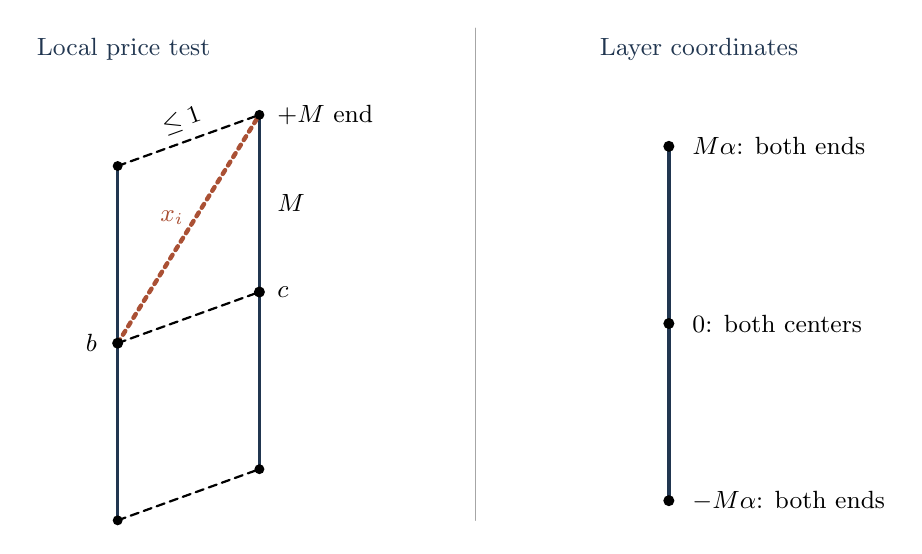
\begin{tikzpicture}[x=1cm,y=1cm,font=\small,line cap=round]
\node[anchor=north west,text=ink] at (-1.15,4) {Local price test};
\draw[ink,very thick] (0,-2.25)--(0,2.25)
  (1.8,-1.6)--(1.8,2.9);
\draw[black,densely dashed,thick]
 (0,-2.25)--(1.8,-1.6) (0,0)--(1.8,.65) (0,2.25)--node[midway,sloped,above] {$\le 1$} (1.8,2.9);
\draw[rust,ultra thick,dotted] (0,0)--(1.8,2.9)
  node[midway,above left,text=rust,inner sep=1pt,fill=white] {$x_i$};
\fill (0,0) circle(2pt) node[left=4pt] {$b$} (0,-2.25) circle(1.8pt)
  (0,2.25) circle(1.8pt);
\fill (1.8,.65) circle(2pt) node[right=3pt] {$c$}
  (1.8,-1.6) circle(1.8pt)
  (1.8,2.9) circle(1.8pt) node[right=3pt] {$+M$ end};
\node[right=3pt] at (1.8,1.78) {$M$};
\draw[gray!70] (4.55,-2.25)--(4.55,4);
\begin{scope}[shift={(7,.25)}]
\node[anchor=north west,text=ink] at (-1,3.75)
  {Layer coordinates};
\draw[ink,very thick] (0,-2.25)--(0,2.25);
\fill (0,0) circle(2pt) node[right=5pt]
  {$0$: both centers}
  (0,-2.25) circle(2pt) node[right=5pt] {$-M\alpha$: both ends}
  (0,2.25) circle(2pt) node[right=5pt] {$M\alpha$: both ends};
\end{scope}
\end{tikzpicture}
\caption{One axis of a tile $b\to c$. In an exact local test (left),
each catalyst segment has length $2M$ and passes through its column
center. Corresponding endpoints are at most one unit apart. For the dotted distance $x_i$, the positive part of $x_i-M$ estimates
the positive displacement along $\alpha$ (Lemma~\ref{lem:protocol-local}). The
fixed layer placement (right) identifies the two centers and each pair
of corresponding ends. In this placement every same-layer link has
price zero.}
\label{fig:altimeter}
\end{figure}

\subsection{Local Euclidean coordinates}

Lemma~\ref{lem:protocol-local} assigns a common coordinate frame to
all the tiles of a single payload path or chain. Its conclusion needs
only the spectral realization on the ball containing that path or chain.
Different balls may use different frames. The layer positions used in
Section~\ref{sec:width} are fixed independently of these local witnesses
(Figure~\ref{fig:altimeter}). Write $u_+=\max\{u,0\}$.

\needspace{10\baselineskip}
\begin{lemma}[Local flattening]\label{lem:protocol-local}
For every $\eta>0$ there exists $M_0$ such that for each integer
$M\ge M_0$ there exists $\varepsilon_M>0$ with the following property.
Consider a payload path or a chain of $H$ tiles in one of the balls
chosen above. If the ball has discrepancy at most $\varepsilon_M$,
assign a point $z_b\in\mathbb R^k$ to each column $b$ of the path or
chain so that the following conditions hold.
\begin{enumerate}
\item The points at the two sides of each fixed identification or
sampler join on the path or chain coincide.
\item For a payload path, its quoted price differs by at most $\eta$
from the distance between its two assigned endpoint points.
If a tested probe joins the endpoints of a chain, their assigned
distance is at most $1+\eta$.
\item For the altimeter $i$ of tile $b\to c$ in signed direction
$\alpha\in\{\pm e_1,\ldots,\pm e_k\}$, set $v_i=(x_i-M)_+$.
Then
\[
 \big|v_i-\langle z_c-z_b,\alpha\rangle_+\big|\le\eta .
\]
\end{enumerate}
The thresholds are uniform in $h,w$, the input permutation and the
chosen path or chain.
\end{lemma}

\begin{proof}
First impose the price constraints exactly. If the conclusion with
tolerance $\eta/2$ fails for unbounded $M$, choose counterexamples with
$M\to\infty$. The degree, ball radius and number of roles are bounded
independently of $M$. Pass to a subsequence with a fixed pattern of
columns, tiles, joins and tested endpoint constraints. Extend the
spectral realizations to complete geodesic $\operatorname{CAT}(0)$
spectral spaces and take their pointed metric ultralimit, based at the
first center. We may take the spectral completion of this ultralimit. Segments
between represented points give geodesics before completion, and
\eqref{eq:wire-busemann} extends them to the completion.
Every involved center lies a bounded distance from that
basepoint, since joins cost zero and center-to-center tile links cost
at most one.

The two opposite ends for each axis at a column have distance $2M$.
Both are within $M$ of its center, so they lie on a segment isometric
to $[-M,M]$ with that center at parameter zero. At bounded parameters
these segments give $k$ oriented lines through the center in the
ultralimit. Along each tile, the same-signed ends of the same axis in
the two columns are within one of each other. Along each join their
distance is zero. By convexity of distance between synchronized
segments this remains true at every finite parameter. Thus the lines
of each axis across all the columns are parallel, with a common
orientation.

At any one column take two different axes. For any signs, the points
at radius $r$ on the two signed half-axes have limiting distance at
most $\sqrt{2}\,r$, since before the limit this distance was at most
$(r/M)\lceil\sqrt{2}\,M\rceil$. In the limit let $u_+,u_-$ be the
opposite radius-$r$ points of the first axis, $o$ their midpoint, and
$v$ either radius-$r$ point of the second. The squared midpoint
inequality gives
\[
 r^2=d(o,v)^2\le
 \tfrac12\big(d(u_+,v)^2+d(u_-,v)^2\big)-r^2.
\]
Both squared distances in the sum are at most $2r^2$, so both equal
$2r^2$. The four points are the corners of a Euclidean square with
diagonals on the two axes. Flat quadrilateral rigidity fills it
isometrically. These filled squares nest as $r$ increases, since the
vertices of each smaller square lie on the diagonals of a larger one
and geodesic uniqueness determines their convex hull. Their union is
a Euclidean plane containing the two axes.

We now place the centers and all their axes in one product
$\mathbb R^k\times Y$ in the ultralimit. The parallel set of the
first axis splits isometrically as $\mathbb R\times Y_1$, with $Y_1$
a complete $\operatorname{CAT}(0)$ space
\cite[Theorem~II.2.14]{BH}. All first axes are line fibers in this
product with the same orientation. Every other axis lies in the
parallel set, because at its column it spans a Euclidean plane with
the first axis. Its line coordinate is constant. Indeed, its point at signed
distance $r$ has squared distance $s^2+r^2$ to the point at signed
distance $s$ on the first axis, for every real $s$. Comparison with
the product distance shows that its first coordinate equals that of
its center. Project the remaining axes to $Y_1$. They are still
synchronously parallel across columns, and the distance equalities for
each pair of axes at a column are preserved. Applying the same
splitting successively gives the stated product, with all $k$ signed
axes aligned. If $Y$ contained two distinct points, the segment between
them times an appropriate cube in $\mathbb R^k$ would contain the
corners of a positive-side-length Euclidean $(k+1)$-cube. The cube
exclusion for spectral spaces under the maximal flat dimension hypothesis
therefore makes $Y$ a point. Let $z_b$ be the Euclidean coordinates
of the limiting centers. Zero-length joins, quoted payload distances
and tested probe caps persist in these coordinates.

It remains to identify a reading involving an endpoint at distance
$M$ from its center. On a unit-speed segment $(p_s)_{0\le s\le M}$ set
$D=d(q,p_0)$ and $E_s=d(q,p_s)-s$. For $0<r<M$ the triangle
inequality gives $E_r\ge E_M$ and $|E_M|\le D$. Squared-distance
comparison at fraction $r/M$ yields
\begin{align*}
 (r+E_r)^2
 &\le (1-r/M)D^2+(r/M)(M+E_M)^2-r(M-r)\\
 &\le r^2+2r E_M+D^2 .
\end{align*}
Consequently $0\le E_r-E_M\le D^2/(2r)$, a finite-segment tail estimate. Take $q$ to be the center of $b$,
$p_0$ the center of $c$, and $p_M$ its $M\alpha$ endpoint.
Here $D\le1$ and $E_M=x_i-M$. At fixed $r$ the ultralimit of
$E_r$ is $\|z_c+r\alpha-z_b\|-r$. As $r\to\infty$, this tends to
$\langle z_c-z_b,\alpha\rangle$. The uniform tail estimate gives that
same limit for $x_i-M$ along the ultrafilter. Taking positive parts
preserves it. The fixed list of limit coordinates consequently
satisfies every constraint with tolerance $\eta/2$ on an
ultrafilter-large set of the original examples, a contradiction.

Finally fix $M\ge M_0$. If no positive discrepancy threshold works,
take counterexamples with discrepancy tending to zero, having the
same labeled ball and chosen path or chain after passage to a
subsequence. The quoted prices lie in a compact box. The scales of
the realizing spectral prices are bounded by the sum of their wire
distances along a core spanning tree, whose edge lengths are bounded
for this fixed $M$. Compactness of the normalized spectrum gives an
exact price test for a limiting price array (including the collapsed
case). Its coordinate assignment with tolerance $\eta/2$ keeps the
joins exactly equal and satisfies all other conditions with tolerance
$\eta$ far enough along the subsequence. This proves uniformity.
\end{proof}

\subsection{Detecting signed motion}

The score has two jobs. High excess at prices consistent with the core
must force many tiles to have large readings in a common signed
direction. A probe connecting the ends of such a chain forces at least
one reading to fall. We weight the squared readings so that this change
contributes more to the divergence in \eqref{eq:protocol-activation}
than the probe's capacity fee. Both signs of every axis are included
because $v_i$ records only positive displacement. The score uses the
readings assigned to the commodities and requires a common Euclidean
frame only along an individual path or chain.

Choose \(\eta=T/(100k)\) and then \(M\) large enough for
Lemma~\ref{lem:protocol-local} for the eventual choices of the sampler
and radius. For any array \(x\) write \(v_i=(x_i-M)_+\) on the altimeter
coordinates. Use the normalized inner product
\(\langle x,y\rangle=n^{-1}\sum_i x_i y_i\). Set
\begin{equation}\label{eq:protocol-score}
 f(x)=c_0\langle x,x\rangle+
       \frac{W^{-4}}{nN}\sum_{i\ {\rm altimeter}}(v_i/T)^2,
 \qquad
 j(s)=W^{-2}\min\{s^{-1},t^{-8}\}.
\end{equation}
Choose a fixed positive rational \(c_0\) small enough that its entire term
is at most \(W^{-4}\) on the box. Indeed the normalized dimension, all
\(a_i\), and \(N,M\) are bounded independently of \(h\). This term supplies
uniform strong convexity. The squared positive part is continuously
differentiable with Lipschitz derivative. Hence the gradient of \(f\) is
Lipschitz with uniformly bounded coordinates, and its \(i\)-th coordinate
vanishes at \(x_i=0\). We have \(f(0)=0\) and
\[
      \int_0^1j(s)\,ds=W^{-2}(1+8W\ln2)\le1
\]
for sufficiently large \(W\). Control can evaluate \(f\) by summing its
coordinate contributions. For fixed rational \(s\), its penalized
maximization separates into one-variable piecewise quadratic problems
on fixed intervals. For each coordinate type, tabulate the summand values
on a grid of mesh \(o(1)\) and the rounded maximizers for every bounded
inventory value on the \(1/w\) mesh. Polynomially many entries in \(h\)
suffice, using \(O(\log h)\) bits per coordinate. Rounding to \(o(1)\)
accuracy before normalized summation gives \(o(1)\) value error, and
uniform coordinate error \(o(1)\) gives \(o(1)\) normalized norm error.
The tables fit the stated word and advice bounds as \(n=2^h\).

For a fixed rational \(s\in(0,1]\) put
\[
                  R_s=\frac{s}{nN}\sum_{i\ {\rm altimeter}}(v_i/T)^2 .
\]
We claim that on any core-consistent sequence of price arrays with
strictly positive lower limit of the excess at \(s\), eventually \(R_s\ge1\).
For \(s<t^8\), all \(0\le v_i\le1\), and hence
\[
   f(x)\le W^{-4}(1+2k/T^2)< W^{-2}t^{-8}=j(s)
\]
once \(W\) is sufficiently large. For \(s\ge t^8\), whenever \(R_s<1\),
\(s f(x)\le 2W^{-4}<s j(s)\). At \(s=1\) we must also bound the mean payload
price. Only \(o(n)\) distinct payload roots have discrepancy exceeding the
fixed threshold from Lemma~\ref{lem:protocol-local}. On every other path
its quoted price is at most \(\eta\) plus the sum of its tile displacements
in its own common Euclidean frame. For a displacement \(z_c-z_b\), the
Euclidean norm equals the square root of the sum of squares of its positive
components along the \(2k\) signed axes. The triangle inequality in
\(\mathbb R^{2k}\) bounds it by
\[
           \left(\sum_{i\ {\rm on\ tile}} v_i^2\right)^{1/2}
                         +\sqrt{2k}\,\eta .
\]
The exceptional payload prices are at most \(N\). Each tile occurs once
among the \(n\) paths. Cauchy--Schwarz on the \(nN\) tiles gives
\[
 \frac1n\sum_{i\ {\rm payload}}x_i
  \le \eta+N\bigl(T\sqrt{R_1}+\sqrt{2k}\,\eta\bigr)+o(1).
\]
For \(R_1<1\) this is less than one for large \(W\), since \(NT=O(t)\).
This excludes each way that the excess could stay strictly positive along
a subsequence with \(R_s<1\).

Mark each tile, when possible, by a signed direction whose altimeter obeys
\[
                       s(v_i/T)^2\ge 1/(4k).
\]
Break ties deterministically. Unmarked tiles together contribute at most
\(1/2\) to \(R_s\), since each has \(2k\) coordinates. A marked tile contributes
at most \(2k/(nNT^2)\). Thus whenever \(R_s\ge1\) there are at least
\(\beta nN\) marked tiles, where \(\beta=T^2/(4k)\).

\subsection{Purchasing the probes}

Within each group form a maximal tile-disjoint collection of chains of
\(H\) tiles having a common mark, joining the output of one tile to the
input of the next by a sampler edge. Different chains may have different
marks. Activate one probe from the first input center to the last output
center of each chain. This is a matching because the tiles have distinct
inputs and distinct outputs. A deterministic scan of all starts and
bounded-length, bounded-degree paths gives a greedy maximal collection
in \(O(n)\) word operations with constants depending on the fixed
parameters. The mark comparisons use only fixed single-coordinate table
lookups. Figure~\ref{fig:marked-probe} depicts the two routes on which
the price test operates.
\begin{figure}[htbp]
\centering
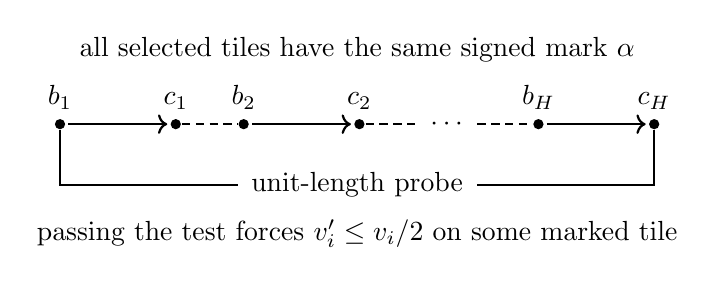
\begin{tikzpicture}[x=0.98cm,y=0.85cm,thick]
  \node at (3.85,1.12) {all selected tiles have the same signed mark \(\alpha\)};
  \foreach \x/\t in {0/{b_1},1.50/{c_1},2.38/{b_2},
                       3.88/{c_2},6.20/{b_H},7.70/{c_H}} {
      \fill (\x,0) circle (1.85pt);
      \node[above] at (\x,0.07) {\(\t\)};
  }
  \draw[->] (0.11,0)--(1.39,0);
  \draw[densely dashed] (1.58,0)--(2.30,0);
  \draw[->] (2.49,0)--(3.77,0);
  \draw[densely dashed] (3.96,0)--(4.62,0);
  \node at (5.01,0) {\(\cdots\)};
  \draw[densely dashed] (5.41,0)--(6.12,0);
  \draw[->] (6.31,0)--(7.59,0);
  \draw (0,-0.08)--(0,-0.91)--(7.70,-0.91)--(7.70,-0.08);
  \node[fill=white,inner xsep=5pt] at (3.85,-0.91)
          {unit-length probe};
  \node at (3.85,-1.64) {passing the test forces \(v'_i\le v_i/2\)
                              on some marked tile};
\end{tikzpicture}
\caption{Signed displacements add along tile arrows because each dashed
join identifies the two adjacent centers. The probe limits the distance
between the first and last centers. The inequality compares an altimeter
reading before and after imposing that endpoint constraint.}
\label{fig:marked-probe}
\end{figure}

Choose \(\delta>0\) sufficiently small that
\(4kH\delta C_W<\beta/2\); this uses only the already fixed stage
parameters. We show that \(\beta nN\) marks yield \(\Omega(n)\) probes.
In a group \(G\), put \(a=\lceil\delta l_G\rceil\). Suppose at least
\(2Ha\) remaining tiles have one fixed mark. Split that many into \(H\)
disjoint sets of size \(2a\). From the first set start with all its
tiles as reachable. If at least \(a\) tiles of one set are reachable,
their distinct output positions have sampler neighbors among all but
fewer than \(a\) of the next set's inputs. Thus at least \(a\) tiles of
every succeeding set are reachable, giving a chain of length \(H\)
and contradicting maximality. Summed over groups, stages, and \(2k\) marks,
the number left is at most
\[
                 4kH\delta C_W nN+o(n).
\]
The ceiling error is \(o(n)\) because \(\min_G l_G\to\infty\) and the total
list length is \(O(n)\) with all stage parameters fixed. Hence at least
\(\Omega(n)\) chains were purchased.

Consider any core-consistent sequence of grid arrays \(x\) with strictly
positive lower limit of the excess, and any sequence \(x'\) consistent
after purchasing those probes. The starting centers of the chains are
distinct roots. All but \(o(n)\) chains therefore admit the coordinate
assignment in Lemma~\ref{lem:protocol-local} at \(x'\). Write
\(v_i'=(x_i'-M)_+\). On each such chain at least one of its marking
coordinates satisfies \(v_i'\le v_i/2\). Otherwise, since \(s\le1\), each
tile would have displacement along the common mark at least
\[
                    T/(4\sqrt{k})-\eta>0 .
\]
Joins have equal coordinates on their two sides, so the sum of the
signed displacements is the signed endpoint displacement. By the choice of \(H\), it exceeds \(1+\eta\), contradicting the imposed probe.

To compare the resulting change in score with the probe fee, observe
that the divergence of $g(u)=(u-M)_+^2$ satisfies
\[
 g(u')-g(u)-g'(u)(u'-u)
        \ \ge\ \big((u'-M)_+-(u-M)_+\big)^2.
\]
This follows by considering the positions of $u$ and $u'$ relative to $M$.
For one of the changed coordinates on each good chain, this inequality
and the marking threshold give a contribution to
\((s/2)\mathcal D_f(x',x)\) of at least
\[
      \frac{sW^{-4}(v_i-v_i')^2}{2nNT^2}
                \ge \frac{W^{-4}}{32k nN}.
\]
The chosen coordinates are distinct, and every other contribution is
nonnegative. Each probe costs \( t^p/n\), which is at most
\(W^{-4}/(64k nN)\) once \(W\) is large enough, since
\(W^4 N t^p=O(W^4t^{p-1})\to0\). With \(\Omega(n)\) chains and only \(o(n)\)
exceptions, the lower limit of \((s/2)\mathcal D_f(x',x)-P\) is strictly
positive. This verifies the activation condition.

All requirements on \(W\) depend only on \(k\) and the initially fixed
protocol parameters. Fix such a \(W\), then the density \(\delta\), the
core-ball radius, \(M\) and \(c_0\), in that order. They are independent
of \(h,w\) and the permutation. Proposition~\ref{prop:adaptive-probing}
now supplies the exact protocols and budget in
Theorem~\ref{thm:protocol}.

\section{Approximate tagged permutations at logarithmic width}\label{sec:width}

Fix the finite field and the maximal flat dimension $k$ of
Theorem~\ref{thm:protocol}. All logarithms in this section are binary.
The tensor $\operatorname{Tag}(h,w)$ tests whether a list of $n=2^h$
tagged $w$-bit records is a permutation of a prescribed list, with each
tag giving the position of its payload in that list
(Definition~\ref{def:tag}). For $w=h$, the two lists together expose
$3nh$ bits. We show that, for every $r>0$, a factor of order $h^r$
above this port count suffices to approximate the test. All data and
tag indices stay exposed, and the size includes the catalyst ports.

\par\Needspace{5\baselineskip}
\begin{theorem}[Approximation at logarithmic payload width]\label{thm:cheaptag}
Under the conclusion of Theorem~\ref{thm:protocol},
for each $r>0$ there is a constant $C$ such that, for all sufficiently
large $h$, $\operatorname{Tag}(h,h)$ admits a trivalent approximation
of size $O(2^h h^{1+r})$ and gap at least
\[
               2^h\,2^{-C(\log(2h))^2}.
\]
In particular its gap is at least $2^h2^{-C'\sqrt h}$ for a fixed $C'$.
\end{theorem}

The proof compares two ways to change the payload width. With wide
payloads, pruning the routing identity saves order $nw$ in the price of
each discarded term, enough to cover the price of summing over tags and
selectors. Each surviving term uses tests with shorter addresses.
Compaction limits the number of tests installed, and amplification
makes their combined error small enough for the parent test. In the
other direction, stable radix sorting implements the width-$h$ test by
packing narrow records into wide ones. The two bounds together force
the overhead exponent at width $h$ to vanish.

\subsection{Compacting active records}

The amplification step corrects a sparse set of records. It has a
fixed array of possible correction slots, but the active positions depend
on the input. We connect the slots to a smaller array of targets in
advance. If at most half the targets are needed, the control can assign
every active slot to a distinct target along these fixed links. Bounded
degree keeps the number of physical alternatives per position constant.
The construction uses probabilistic expansion (see \cite{HLW}).

\begin{lemma}[Compaction with slack]\label{lem:slack-compaction}
Fix $C\ge1$. For $m\le CK$ slots and $K$ targets there is a bipartite
graph with degrees bounded in terms of $C$, on which any set of at most
$K/2$ active slots has an injective assignment to neighboring targets.
Given the graph as fixed advice, the assignment can be chosen
deterministically in $O_C(K)$ word operations on $O(\log(2K))$-bit words.
\end{lemma}

\begin{proof}
For bounded $K$ use the complete bipartite graph. For large $K$, fix a small $\Delta>0$ depending
on $C$. Keep $R=\lfloor K/4\rfloor$ targets in reserve. A bounded-choice
graph on the other targets can make every $\lceil\Delta K\rceil$ slots
meet every set of $\lceil K/5\rceil$ targets. Indeed, give each slot
$d$ random choices. The probability of missing a fixed pair of sets
is at most $(1-1/5)^{d\lceil\Delta K\rceil}$, and there are at most
$2^{(C+1)K}$ pairs. Choose $d$ large enough. Process the active
slots in order, taking the first free neighbor if there is one.
At least $K/5$ targets remain permanently free on this side. No
unmatched slot is adjacent to any of them, so fewer than
$\lceil\Delta K\rceil$ slots remain.

Independently give each slot eight choices in the reserve. For
$1\le l\le\Delta K$, the probability that some $l$ slots have at most
$4l$ distinct neighbors is at most
\[
   \binom{m}{l}\binom{R}{4l}(4l/R)^{8l}
          \le \bigl(C_1(l/K)^3\bigr)^l
\]
after increasing $C_1=C_1(C)$. Here the exponent is $8-4-1=3$. Take $\Delta$ small enough that
$4\Delta K\le R$ and $C_1\Delta^3<1/2$ for large $K$.
Splitting the sum at $l=\sqrt K$ shows its convergence to zero.
To bound the target degrees in both random constructions, partition
the slots in each choice layer into blocks the size of the relevant
target set. Use an independent random permutation within each padded block. Within each block, sampling without replacement bounds the probability of
landing entirely in a given subset by the corresponding with-replacement
probability. Thus both bounds still hold, and a target occurs at most once
per block per layer.

Among $l>0$ remaining slots in the reserve graph some target has
degree one on their incidences, since there are more than $4l$
neighbors and only $8l$ incidences. Assign its unique slot to it
and delete that slot with its incidences. A fixed-order queue of
degree-one targets and incidence lists maintain this operation in
linear time, skipping stale queue entries. The assigned targets are
distinct. The queue, the incidence scans and the greedy first pass fit the word
bounds of Definition~\ref{def:protocol}.
\end{proof}


\subsection{Amplification by sparse exact corrections}

To amplify the gap for a batch of tagged tests, we will evaluate a
small fraction of the tests exactly. We begin with the cost of one such
evaluation.

A single exact tagged test costs $O(nwh)$ for $w\ge h$. Indeed, an AKS
sorting network uses $O(nh)$ comparators to sort the second list by tag
\cite{AKS}. Comparing two tags and routing their payloads costs
$O(h+w)$ bit gates, including fan-out. Compare the sorted tags with the
prescribed positions and the sorted payloads with the first list.
The resulting Boolean verification gives an exact trivalent tensor
network over every field. A stable sort on $2^d$ records of $v$ bits
also has a network consisting of one $\operatorname{Tag}(d,v)$ call and
$O(2^d(d+v))$ additional size. Guess an input position for each proposed
output, check the permutation of the payloads with the call, and check
nondecreasing keys with increasing input position at ties. Each valid
input--output pair has exactly one witness.

\begin{lemma}[Amplification]\label{lem:tag-amplification}
Let $X$ approximate $f=\operatorname{Tag}(h,w)$ with exposed data, size
$S$, and gap $D$ (using a trivalent realization of $X$), where $w\ge h$ and $D\ge4k(\log h+3)$. Fix $C'>0$.
For all sufficiently large $h$ and every integer $s\ge1$ with
$\log s\le h^{C'}$, the tensor $f^{\otimes s}$ has a trivalent
approximation of size at most $C_{\rm amp}sS$ and gap at least
$sD/(2h)$. The size constant is absolute. The threshold for $h$ may
depend on $C'$ and $k$.
\end{lemma}

\begin{proof}
Truncate the tensor-power expansion by the number of errors. The
discarded terms contain enough errors to give the amplified gap, and the
retained terms require exact corrections at only a small fraction of
positions. Let $I$ be the through identity on the catalyst of $X$ and put
$F_0=f\otimes I$, $E=F_0-X$. In $(X+E)^{\otimes s}$ retain precisely
the terms with at most $p=\lfloor s/h\rfloor$ copies of $E$. Give this
sum the catalyst format of $s$ copies of $X$.

Fix a price $H=c\log\varphi$ on the center and the $2k$ unit catalyst
sites, induced by any spectral $k$-flat. Its scale satisfies $c\le2k$, by the star through the center.
Normalize spectral values of one copy by $\varphi(I)$. The normalized
values of $F_0,E,X$ are at most $1,z,1+z$, respectively, where
$z=2^{-D/c}$. Here ordinary sum is a restriction of direct sum, and
multiplication by a nonzero scalar preserves the price. Exact $X$ can
be powered directly. For finite $D$ we have $z\le1/h$. Weight each
omitted term with $j$ errors by $(hz)^{-j}$, and use multiplicativity
and the binomial theorem. The sum of the normalized values of all
omitted terms is at most
\[
                 (hz)^{p+1}(1+z+1/h)^s .
\]
This bounds the spectral value of the error relative to
$\varphi(I)^s$. Since $p+1\ge s/h$ and
$\log(1+z+1/h)\le (2\log e)/h<3/h$, the price discount is at least
\[
         \frac{s}{h}\bigl(D-c(\log h+3)\bigr)\ge \frac{sD}{2h}.
\]

For the size assertion, encode each position by one of three choices,
namely ordinary $X$, a selected correction $F_0$, or a selected
correction $-X$. Reject strings with more than $p$ selected positions. This gives
one encoding for each summand of the retained expansion after expanding
$E=F_0-X$. Put a switchable copy of $X$ at every position. A switched-off
module has every internal bit fixed to zero and local value one on
that assignment. This is implemented with a copied enable bit on its
bounded-arity tables and equality vertices if a wire requires one.
A position assigned $F_0$ bypasses its own catalyst bits by through
wires and routes only its $O(nw)$ data bits to an exact $f$ module.
Assign the sign locally at each selected $-X$. All unused fields and
inactive lanes have a unique zero padding.

If $p=0$, use $X^{\otimes s}$.
Otherwise, repeatedly halve the list length, rounding up, until at most
$4p$ positions remain. At every actual halving there are at most $p$
active positions and the destination length is at least $2p$.
The bounded-degree compaction graph for ratio two and its deterministic linear-word-time assignment algorithm (Lemma~\ref{lem:slack-compaction}) send the active positions injectively to neighbors.
Use the chosen switches for the whole data word of a position.
The sum of the list lengths is $O(s)$, hence data routing, including
its interface to the local $X$ modules, costs $O(snw)$. Install exact,
switchable $f$ modules at the final list, costing $O(pnwh)=O(snw)$.
All graph descriptions have $O(s)$ words of advice. The configuration
algorithm and the check on the number of selected positions use
$O(s)$ operations on $O(\log(2s))$-bit words. Verify the deterministic memory trace by sorting its records by address
and time with a Batcher network \cite{Batcher}. A scan in this order
checks each read against the initialization or the most recent write, as
in RAM verification for proof systems \cite{TinyRAM}. Chronology, unused records, and final configurations
have fixed conventions, so each legal choice has one history.
This control costs $O(s\,\mathrm{polylog}(2s))=O(snw)$ because the fixed
power of $\log(2s)$ is eventually bounded by $2^h$ in the stated
range. The implied size constants are absolute. Each exposed network
has $S\ge nw$, and all enable wires and catalyst bypasses cost $O(sS)$.
\end{proof}

\subsection{The width profile and stable radix packing}

For a polynomial payload width $w=\lceil h^a\rceil$, measure the size
as an overhead above $nw$, keeping the required gap essentially
proportional to the list length. Put $L(h)=\log(2h)$. For $a\ge1$,
define $r(a)$ as the infimum of the
real $r$ such that for some $C>0$ and all sufficiently large $h$ the
tensor at width $w=\lceil h^a\rceil$ admits exposed approximations of
size $O(nw h^r)$ and gap $n2^{-C L(h)^2}$ or greater. Write
$r_*=r(1)$ and $r_\infty=\inf_{a\ge1}r(a)$. The port count and the
exact construction give $0\le r(a)\le1$. Pinning matching padding
bits to zero makes a wide test serve a narrower payload. For the
reverse operation, split the wide payload into slices, copy the tags
to every slice, and multiply the predicates. This product enforces
the permutation condition on the common tags and every payload equality. The tag copies cost $O(nh)$ per slice.
For any fixed $a'\ge a$ the number of slices is polynomial in $h$.
Lemma~\ref{lem:substitution} loses at most $2k$ times that number
in absolute gap, absorbed by increasing $C$. Thus
\[
                  0\le r(a)-r(a')\le a'-a .
\]
The same argument permits constant factors in the width at fixed $a$.

In a radix sort, the digit length controls the cost of sorting a block,
whereas the pack width controls the cost of moving many records with
the same digit. Optimizing these two costs separately gives an upper
bound on $r_*$ in terms of the profile at larger widths.

\begin{proposition}[Packing wide records]\label{prop:tag-width-packing}
For every fixed $a>1$,
\[
 r_*\le 1-\frac1a+\max\{r(a)/a,r_\infty\}.
\]
\end{proposition}

\begin{proof}
To check the parent tagged relation, stably radix-sort a combined list
of sources and targets
with their keys and record-type flags and use a final scan to check for one
matching payload of each type at each tag. This list has $\Theta(n)$
records of $O(h)$ bits. Take $k_0=\lfloor h^{1/a}\rfloor$ digit bits per
pass, proceeding from least significant to most significant. For any
fixed $B>1$, take a dyadic pack size $P$ in $[h^{B-1},2h^{B-1})$.

Pad to blocks of $2^{2k_0}$ slots and stably sort each block on its
current digit, placing dummies last. Round each nonempty digit run up
to a multiple of $P$ and place its first real record at a multiple of
$P$. The original slots already accommodate the old dummies. Rounding and
alignment require only $O((2^{k_0}+1)P)$ additional slots per block. Scans compute run lengths, rounded
lengths, and destinations (including for old dummies) in $O(h)$ per slot. A second tagged transport implements the alignment. For instance, give each source its destination as a tag (transpose the perspective on which list is in prescribed order). Positions not yet assigned are filled with padding sources in increasing order; this last condition is enforced by carrying source positions as part of the payload and checking on the output side that those sources are in order. When a
tagged call is padded to a power of two, pin the payload on both sides
of each extra slot to zero and fix its output tag to the address of its
own input slot. The padded matching thus extends the original one
uniquely. All real records in a pack now have the same digit. Obtain the key of each nonempty pack
by a scan, stably sort the packs by that key with empty packs last, and
retain the order of real records within the packs. The result is the
stable sort on this digit among real records; scans ignore vacant slots and move forward across them. The list length grows each pass by a fraction
$O(2^{-k_0}P)$ and an additive $O(2^{2k_0}+2^{k_0}P)$ for the partial
block. Over $O(h/k_0)$ passes it stays $\Theta(n)$, with lengths fixed
before receiving the data.

There are a constant number of collections of block calls per pass,
each of common address length $l=2k_0+O(1)$, payload width $O(h)$ and
$\Theta(n)$ slots in total. Implement a block at the bound for $r(a)+e$,
$e>0$, with matching constant-factor width adjustments. Amplify its
$s=\Theta(n/2^l)$ copies by Lemma~\ref{lem:tag-amplification}, using
$\log s\le h=l^{O_a(1)}$. Each collection costs
$O(nh\,h^{(r(a)+e)/a})$ and has gap at least
$\Omega(n2^{-C L(l)^2}/l)$ for a constant $C$.
Each pass also uses one pack sort with $\Theta(n/P)$ slots, address
length $h-O(\log h)$ and width $O(hP)$. The bound at $r(B)+e$ costs
$O(nh\,h^{r(B)+e})$ and gives gap at least $n2^{-C_1 L(h)^2}$ after
enlarging $C_1$ to absorb the factor $P$. The scans and tag copying cost
$O(nh)$ per pass. Treat each collection of block calls as one product
gate, as allowed for a multilinear tensor contraction. Across all passes
there are polynomially many substituted gates, and the gaps dominate
their number. A further increase of $C_1$ makes the result admissible in
the width profile. Multiply the size bounds by $O(h^{1-1/a})$, let
$e\downarrow0$, and take the infimum over $B>1$.
\end{proof}

\subsection{Pruning the routing identity and counting shorter calls}

For a valid tag assignment $\pi$, denote by $M_\pi$ the payload
matching tensor with entries $\prod_i\mathbf{1}_{q_i=p_{\pi(i)}}$,
and by $\delta_\pi$ the basis tensor supported on that assignment to
the tag ports. Definition~\ref{def:protocol} supplies an exact routing
identity for $M_\pi\otimes I$, where $I$ denotes the protocol catalyst
identity. Tensor each routing identity with $\delta_\pi$ at the origin
and sum over permutations. The resulting tensor is exactly
\[
 \sum_{\pi\in S_n}\delta_\pi\otimes M_\pi\otimes I
       =\operatorname{Tag}(h,w)\otimes I.
\]
In a network this sum is implemented by checking that the exposed tags
form a permutation and using those tags in the control. Each valid tag
assignment activates its own routing identity with the original selector
multiplicities. This representation also places the error from pruning
different tag assignments on the same set of exposed ports.

Fix $\kappa>0$ and $A>1+\kappa$, and take $h^{1+\kappa}\le w\le h^A$. Retain the terms for which
the sum of $\lambda y$ over links joining different layers is at least
$2MN_c/w-n$. To price one discarded term, place its sites at their layer
coordinates divided by $M$ in the unit catalyst configuration on any
spectral $k$-flat. Local tensors and same-layer links cost zero.
Every cross-layer link costs at most $\lambda yw/M$ since its charge
dominates its Euclidean layer distance. The local factor $\delta_\pi$
has price zero. Thus a discarded term has
price at most $2N_c-nw/M$. Across all valid permutations and all
selectors there are at most $2^{O(nh\,\mathrm{polylog}\,h)}$ terms.
The cost of their sum is at most their maximum price plus
$O_k(nh\,\mathrm{polylog}\,h)=o(nw)$. Consequently the surviving
contraction approximates $\operatorname{Tag}(h,w)$ with exposed gap
$\Omega(nw)$ relative to the through price $2N_c$. Testing the pruning
condition adds only linear word work using the fixed rational charges.
Each surviving term satisfies
\begin{equation}\label{eq:tag-positive-budget}
            \sum_{t>0}(\lambda y+t^p)\le 11n .
\end{equation}


We next turn the surviving traffic bound into a recursion for network
size. Let $u:[1,\infty)\to(0,\infty)$ be a smooth, eventually constant
function with $u(1)>r_*$ and $0\le-u'<1$. We will prove $r(a)\le u(a)$
by induction on address length. The width-$h$ estimate starts the
induction near $a=1$. For wider payloads, the shorter calls must fit
inside the parent allowance $nwh^{u(a)}$.

Write $a=\log_h w$, $b=-u'(a)$ and $v=u(a)+ab$, and fix
$\epsilon>0$. When a child call uses fractions $T$ and $Y$ of
the parent's address length and payload width, its size allowance
\emph{per slot}, relative to the parent's, is asymptotic to
\[
                          T^v Y^{1-b}.
\]
Indeed the width exponent changes from $a$ to $\log_{Th}(Yw)$.
The calculation after \eqref{eq:tag-uniform-width} gives the uniform
estimate. Since $v-b=u(a)+(a-1)b>0$, we can choose $Y=T^p$ with $p>1$
close to one so that $v-pb>0$ uniformly. Even with order $n/Y$ installed
slots the relative cost is then $O(T^{v-pb})$, which tends to zero
as $T$ decreases. Equation~\eqref{eq:tag-positive-budget}
bounds the active slots in each summand. Compaction turns this into a
bound on the number of slots installed in the common network.

\begin{lemma}[Shorter calls]\label{lem:tag-shorter}
One choice of protocol parameters works for all sufficiently
large $h$ and $1+\kappa\le a\le A$. The pruned contraction is implemented
exactly relative to the following tagged calls, with fixed positions and
wiring for each format.
\begin{enumerate}
\item A fixed finite menu of dyadic pairs $(T,Y)$ has $0<T\le1/2$,
$0<Y\le1$. At each installed type the calls have common address length
$h'=Th+o(h)$ and width $w'=\lceil Yw\rceil$. Counting all physical
slots, including idle slots, their numbers $S_{T,Y}$ satisfy
\[
       S_{T,Y}=\Omega(n)\quad\text{per type},\qquad
       \sum_{T,Y} S_{T,Y} T^v Y^{1-b}\le\epsilon n .
\]
\item A bounded number of control calls have address length
$h+O(\log h)$, width equal to address length, and
$O(n\,\mathrm{polylog}\,h)$ slots altogether.
\end{enumerate}
All other gates and wires, including the incidences at the calls, cost
$O(nw\,\mathrm{polylog}\,h)$.
\end{lemma}

\begin{proof}
The continuous function $v-b=u(a)+(a-1)b$ has positive minimum
on $[1+\kappa,A]$. Choose a rational $p>1$ sufficiently close to one
that $v-pb$ still has positive minimum. Take $W$ large enough for
Theorem~\ref{thm:protocol}, with $pW$ integral, and use a single type
$(T,Y)$ given by
\[
 T=2^{-W},\qquad Y=T^p.
\]
Scale-zero groups have bounded size and are wired with switches. For the scale-$T$ groups, orient links and reserve distinct source and destination slots. Split each nonempty link into transports of width $\lceil Y w\rceil$, padding its last chunk; protocol bounds allow us to reserve fixed numbers of slots for these chunks. By \eqref{eq:tag-positive-budget} at most $c_*n$ transports are used in any one summand, where $c_*=22 T^{-p}$. Hence for $W$ sufficiently large
\[
 7c_* T^v Y^{1-b}\le\epsilon
\]
uniformly in $a$.
Pack whole groups by next fit into dyadic supergroups of
size $H_0=2^{Th+o(h)}$, at least twice the largest group size after slot
duplication. This uses $O(n/H_0+1)$ supergroups. Take $K$ a sufficiently
small fixed dyadic fraction of $H_0$. List transports in each supergroup
in canonical order in batches of at most $K/2$, filling all but the last.
Reserving $K$ positions per nonempty batch uses in total at most
$2c_*n+O((n/H_0+1)K)\le3c_*n$ positions. This choice uses the uniform
lower bound on $c_*$ and $H_0=o(n)$.

Hardwire candidate batches for every supergroup, allowing all its slots
to be active. For each batch, Lemma~\ref{lem:slack-compaction} assigns active source and destination slots separately to two $K$-slot
lists by bounded-degree switches. Apply the same lemma to the set of
nonempty batches, assigning each entire pair of lists to one of
$\lceil6c_*n/K\rceil$ physical modules. The number of candidates is
$O(n/H_0+1)$, a bounded multiple of the number of modules, and at most
half the modules are needed for any summand. One
$\operatorname{Tag}(\log K,\lceil Yw\rceil)$ in each occupied module
has its tags set to the actual matching of the two lists. For the remaining
slots, set the tags to match the vacant destinations with vacant sources
in increasing order and fix all unused payload bits to zero. Idle modules
use the identity permutation and zero data. Thus every original link is
enforced with its prescribed multiplicity. There are between $6c_*n$
and $7c_*n$ installed slots for large $h$. This gives the weighted slot bound.

All assignment graphs are fixed advice of linear word size for fixed
parameters. Scans compute the active lists, the deterministic assignments
and the completed permutations in $O(n\,\mathrm{polylog}\,h)$ word
operations, including a scan of each candidate link to a $K$-slot
batch. Whole-batch switches transport $O(K\lceil Yw\rceil)$ bits per
incidence, while individual slot switches transport $O(\lceil Yw\rceil)$
bits. The number of incidences per position is bounded for fixed
parameters. Variable subfield shifts cost $O(w\log(2w))$ per site.
Together with the site networks, pins, selector copies and outside
catalyst ports these fit $O(nw\,\mathrm{polylog}\,h)$. For protocol
control, guess a timed RAM history and check each bounded-word step.
Sort the memory records, including initialization, by address and time
and scan them to verify that reads agree with the latest value. Pad the
history canonically and resolve ties by the step's fixed access order.
This leaves one history for each deterministic computation. Tag validity
can be tested by one more sort. A bounded
number of stable sorts use $O(n\,\mathrm{polylog}\,h)$ slots with
$O(h)$-bit records. Pad lengths to powers of two of address length at
least $h$, and split records into a bounded number of address-width
slices with shared tags. This gives the claimed control calls and
$O(nh\,\mathrm{polylog}\,h)$ further size.
\end{proof}

\subsection{Closing the induction}

Fix $u$ as above and choose $A$ sufficiently large in the interior of
its constant region. We prove the size and gap estimates together by
strong induction on the address length $h$. For every integer $h\ge2$
and every integer $w$ with
$h\le w\le h^A$, there are approximations with
\begin{equation}\label{eq:tag-uniform-width}
  \text{size}\le D_{\rm cost}\,2^h w h^{u(\log_h w)},\qquad
  \text{gap}\ge D_h=2^h\,2^{-C_{\rm gap}L(h)^2}.
\end{equation}
Choose $r_*<r'<u(1)$ and $\kappa>0$ small enough that $r'<u(a)$ on
$[1,1+\kappa]$. Fix $C_{\rm gap}>3$ strictly larger than the constant
in the width-$h$ estimate for $r'$. On this narrow-width interval,
slicing the payload into $\lceil w/h\rceil$ padded width-$h$ tests
proves \eqref{eq:tag-uniform-width} for sufficiently large $h$ with
any $D_{\rm cost}\ge1$. The strict margins absorb the slicing constants
and the polynomial absolute gap loss.

For $1+\kappa\le a\le A$, apply Lemma~\ref{lem:tag-shorter} with
$C_{\rm amp}\epsilon<1/4$. Use the $r'$ estimate for the control calls, whose payload
width equals their address length. Their gaps are $\omega(D_h)$ because their address
length is $h+O(\log h)$ and the exponent constant has a strict margin.
Every shorter type has $h'<h$ and $w'>h'$ for large $h$. If
$w'>(h')^A$, split into
$\lceil w'/\lfloor(h')^A\rfloor\rceil$ nearly equal integer slices.
There are boundedly many, each of width exponent $A+o(1)$ at height
$h'$, hence within the constant region. Treat each type as a single
batch of $s=S_{T,Y}/2^{h'}$ identical calls, separately for each
slice. Induction at $h'$ and Lemma~\ref{lem:tag-amplification} give
each batch gap at least
\[
          \frac{sD_{h'}}{2h'}
           =\Omega\left(\frac{n\,2^{-C_{\rm gap}L(h')^2}}{h'}\right)
           =\omega(D_h).
\]
Indeed $h'=Th+o(h)$ uniformly on the fixed menu, $T\le1/2$, and
$L(h)^2-L(h')^2\ge(2-o(1))\log h$. Also $\log s=O(h)$ and $D_{h'}$
exceeds the amplification threshold. The outer pruned gap is $\Omega(nw)$. Each amplified batch enters
the parent contraction as a single product gate. Thus
Lemma~\ref{lem:substitution} charges once per type and slice, and once
per control call. Their total number is bounded, so the resulting gap
is at least $D_h$ for sufficiently large $h$.

The ratio of the shorter per-slot size allowance to the parent allowance,
including the amplification factor, is
\[
 C_{\rm amp}\frac{w'(h')^{u(\log_{h'} w')}}{w h^{u(a)}}
        =(1+o(1)) C_{\rm amp}T^vY^{1-b}.
\]
In fact $\log h'=\log h+\log T+o(1)$ and
\[
 \log_{h'}w'-a=\frac{\log Y-a\log T+o(1)}{\log h}.
\]
Taylor expansion with $u'(a)=-b$ proves the formula uniformly on the
compact interval and fixed menu. For the split case the exponent is
constant and the slice widths sum to $w'$, giving the same allowance.
The shorter-call work consumes at most half the proposed size for large
$h$. For the remaining ordinary work and control costs we have
\[
 nw\,\mathrm{polylog}\,h+nh^{1+r'}\mathrm{polylog}\,h
                      =o(nwh^{u(a)}),
\]
since $u$ has positive minimum on the interval and
$a+u(a)\ge1+u(1)>1+r'$. This also pays for extra tag copying when
splitting calls. All thresholds are independent of $D_{\rm cost}\ge1$.
An enlargement of $D_{\rm cost}$ covers the finitely many smaller
formats using exact networks. This completes the induction.

\begin{proof}[Proof of Theorem~\ref{thm:cheaptag}]
Taking $A$ arbitrarily far into the constant region in
\eqref{eq:tag-uniform-width} gives $r(a)\le u(a)$ for every fixed $a$.
If $r_*>0$, we can choose $u$ to decrease fast enough just above
$a=1$, and to level off low enough at large $a$, that both terms in
the packing bound improve on $r_*$. To do so, choose $1-r_*<b_0<1$, and choose $t>0$ sufficiently
small and $0<e_0<(r_*+b_0-1)t$. On $[1,1+t]$ take
$u(a)=r_*+e_0-b_0(a-1)$ and extend it smoothly to the positive plateau
$r_*/3$ with $0\le-u'<1$. For small $t$, the linear piece stays above
the plateau and $t/(1+t)+r_*/3<r_*$. Also
$(t+u(1+t))/(1+t)<r_*$ by the choice of $e_0$. In
Proposition~\ref{prop:tag-width-packing} with $a=1+t$ substitute
$r(1+t)\le u(1+t)$ and $r_\infty\le r_*/3$. The right-hand side is
strictly less than $r_*$. Hence $r_*=0$, which gives the assertion
for every fixed $r>0$ by the definition of the profile.
\end{proof}

\part{Descent and contradiction}
\section{Port graphs from cube exclusion}\label{sec:ports}

Network compression can bring many wires to a single vertex. To restore
bounded degree, Section~\ref{subsec:refresh} replaces all-pairs demands
among that vertex's ports by wires on a sparse graph. The metric estimate
this replacement requires is a Poincar\'e inequality, uniform over all
spectral placements of the ports. We show that the cube exclusion of
Section~\ref{sec:prices} gives graphs with precisely this property.

Let $G$ be a symmetric stochastic matrix on a finite vertex set $V$
and assign a point $x_i$ of a spectral space to each vertex $i$. The
mean squared length of a step of $G$ and the mean squared distance
between two independent uniform vertices are, respectively,
\[
 \mathcal E_G(x)=\frac1{|V|}\sum_{i,j\in V}G_{ij}d(x_i,x_j)^2,
 \qquad
 \mathcal V(x)=\frac1{|V|^2}\sum_{i,j\in V}d(x_i,x_j)^2.
\]

\begin{definition}\label{def:ports}
A field \emph{has ports} if it admits a family of regular, symmetric
multigraphs of unbounded order and bounded degree, and a constant
$\gamma$ such that
\[
 \mathcal V(x)\le\gamma\mathcal E_G(x)
\]
for every graph in the family and every assignment into a spectral space
over the field. Here $G$ denotes normalized adjacency. A diagonal arc
keeps the walk at its current vertex.
\end{definition}
This property depends only on the characteristic, since it concerns
only joint prices of binary wires (Lemma~\ref{lem:comparison}).
By Theorem~\ref{thm:geometry} one may test either finite spectral
points or complete $\operatorname{CAT}(0)$ spectral spaces. Testing
an assignment that is constant on each of two components and takes two
distinct values shows that every port graph is connected.

For use in Section~\ref{subsec:refresh}, we may take the graphs to be
loopless, of arbitrarily large power-of-two order and of one fixed
power-of-two degree. Given a graph of order $M$, duplicate enough
vertices to reach the next power of two. Keep the old edges between
the original representatives, join each duplicate to its representative,
and pad with holding arcs to a fixed power-of-two degree. To compare any
pair, follow the path through its two representatives. A uniform endpoint
chooses any particular representative with probability at most $2/M$.
The mean squared distance from a vertex to its representative is controlled
by a constant times the new edge energy, since each such pair is an edge
and the degree is bounded. The triangle inequality therefore gives a
uniform Poincar\'e bound after duplication. To remove loops, take two
copies of this graph. Replace each holding arc by a crossing to the
corresponding vertex in the other copy, and join every such pair of vertices
by as many additional parallel edges as the previous degree. The degree
doubles. The same comparison through representatives again gives a
uniform bound.

\begin{proposition}\label{lem:refresh-graph}\label{lem:ports}
If a finite field $F$ has a largest spectral flat dimension $k$, then
$F$ has ports.
\end{proposition}

\subsection{Construction of the port graphs}\label{app:refresh-graph}

The proof of Proposition~\ref{lem:refresh-graph} starts on a finite
Grassmannian. The quadrilateral inequality gives an upper bound on the
mean squared distance between complementary subspaces in terms of the
mean for adjacent ones. Equality would realize the excluded cube, so
there is a uniform gain. We use this gain twice. First, it yields sparse
matrices whose Poincar\'e constants grow more slowly than the exponent
governing their orders. Then a graph product turns this disparity into
a uniform bound at fixed degree.

The product uses the two equally weighted sets of transitions in the
balanced replacement product of Reingold, Vadhan and Wigderson
\cite[Definition~6.6]{RVW}. For the corresponding nonlinear spectral
comparison, see Mendel and Naor \cite[Theorem~1.13(V) and \S8]{MendelNaor}.
Their Ces\'aro estimates for the two-map nonlinear spectral gap in Hadamard
spaces appear in \cite[Corollary~1.9]{MendelNaorBarycentric}
and \cite[Theorem~3.4]{MendelNaorHadamard}. We give the one-map
lazy-walk estimate with the constants needed here.

Let $\mathcal X_F$ be the class of complete $\operatorname{CAT}(0)$
spectral spaces over $F$. By Theorem~\ref{thm:geometry}, every spectral
wire pseudometric embeds in a member of $\mathcal X_F$ after identifying
points at distance zero. Completeness permits us to take barycenters.
Write $\ell=k+1$ and let $Q_\ell=\{0,1\}^\ell$ be the excluded set of
cube corners with the Euclidean metric. Squared distances on $Q_\ell$
are Hamming distances. A matrix
$G$ has \emph{bound} $\gamma$ if $\mathcal V(x)\le\gamma\mathcal E_G(x)$
for every assignment into every member of $\mathcal X_F$. In a regular
graph we count both directions of an edge and count a loop as one diagonal
arc.

\subsubsection{A strict inequality on the Grassmannian}
Fix a power of two $m>\ell$, put
$W=\mathbb F_2^{2m}$, and let $\mathcal G$ consist of its $m$-dimensional
subspaces. The binary field here indexes the subspaces. Their images
lie in a spectral space over the coefficient field $F$, of arbitrary
characteristic. Given a map of $\mathcal G$ into $X$, let $B_r$ be the mean
squared distance over ordered pairs $(U,V)$ with $\dim(U+V)=m+r$.
Thus $B_1$ averages over adjacent subspaces, which meet in a hyperplane
of each, while $B_m$ averages over complementary subspaces.

\begin{lemma}\label{lem:wire-grassmann-gap}\label{lem:grassmann-gap}
There is an $\eta>0$, independent of $X\in\mathcal X_F$ and the map, such
that $B_m\le(m-\eta)B_1$.
\end{lemma}

\begin{proof}
By \eqref{eq:cur-quad}, the sum of the two squared diagonals of a
quadrilateral is at most the sum of the four squared sides. At
equality its opposite sides have equal lengths, as shown after
\eqref{eq:cur-quad}.

For $r,s>0$ with $r+s\le m$, take spaces $K,R_0,R_1,S_0,S_1$ in direct
sum of respective dimensions $m-r-s,r,r,s,s$. The four spaces
$K+R_i+S_j$ form a quadrilateral indexed by $i,j\in\{0,1\}$. Under a
uniform random automorphism of $W$, each ordered pair is uniform on all
pairs with its given sum dimension. Averaging the quadrilateral inequality
yields
\[
 B_{r+s}\le B_r+B_s,\qquad B_r\le rB_1.
\]
Suppose for a moment that $B_1=1$ and $B_m=m$. Then $B_r=r$ for every
$r$, by $B_m\le B_r+B_{m-r}$ for $0<r<m$. Every quadrilateral just used
is an equality configuration, since the deficits of all its translates are nonnegative
and have average zero.

Fix $0<r<m$ and independent columns $u_1,\ldots,u_r,w_1,\ldots,w_r$ in
$W$, with respective spans $U,U'$. Complete them by $m-r$ further
independent columns of span $S$. The image distance between $S+U$ and
$S+U'$ is independent of this choice of completion. Indeed, replacing one
completion column by a vector outside the current total span preserves the
distance by equality of opposite sides in the quadrilateral of type
$(r,1)$. These replacements connect all completions. To see this, for any
independent tuple of length less than $2m$ with a fixed prescribed
subtuple, one can simulate any independence-preserving change of a single
free column by these replacements. If the desired new column belongs to
the present span, first replace the old one by a vector outside the span.
This puts the desired column outside the new span. Arbitrary
independence-preserving changes connect the tuples by extending them to full
bases and using elementary column operations fixing the prescribed subtuple.
These are generated by additions on the remaining columns over
$\mathbb F_2$ (first modulo the prescribed subspace, then adding its
columns). Record only the changes to the original tuple.

The resulting common distance is also invariant when one of the $2r$
original columns $z$ is changed to a column $z'$ outside their span.
For this move choose the completion to contain $z+z'$ and extend it independently. The
total spans before and after this choice are the same, and neither
$S+U$ nor $S+U'$ changes. Since $2r<2m$, connectivity of the column
moves applies again. Every pair with sum dimension $m+r$ has such a
presentation, so every such squared distance equals $B_r=r$.

Choose $\ell$ disjoint pairs of columns and another $m-\ell$ columns,
all independent. The spaces spanned by the common columns and one choice
from each pair have squared image distances equal to the number of
differing choices, since $\ell<m$. Their images are an isometric copy
of $Q_\ell$.

Finally, if $B_1=0$ then $B_m=0$. If the asserted strict uniform gap
failed, we could rescale a sequence of configurations to have $B_1=1$
and $B_m\to m$. All entries of the finite distance arrays are bounded since
$B_r\le rB_1$ for every $r$. Take a convergent subsequence. Every array
is realizable up to scale over $F$, so the ultralimit procedure of Section~\ref{sec:limits}
realizes its limit up to scale as well. In a corresponding rescaled
geodesic completion this limiting map has $B_1=1$ and $B_m=m$. The
equality argument produces the excluded $Q_\ell$, a contradiction.
\end{proof}

\subsubsection{Sparse matrices on rapidly growing sets}
Decrease $\eta$ if necessary and choose $\varepsilon>0$ so that
$1<\alpha=(m-\eta)(1+\varepsilon)<m$. For every power of two $D\ge2$
and every integer $j\ge0$, we construct a symmetric stochastic matrix on
$D^{m^j}$ vertices with at most $C_jD$ entries in the support of each row
and with bound $C'\alpha^j$. Here $C_j$ may depend on $j$, whereas $C'$
is independent of both $j$ and $D$.

Start with the uniform matrix at size $D$. Given a matrix at size $N$,
let $E=\mathbb F_2^{\log_2 N}$ and take $\Omega=E^m$ as the new vertex
set. Fix an ordered basis in each $U\in\mathcal G$. A uniformly random
linear map $W\to E$ defines a uniform vertex of $\Omega$ at each $U$ by
reading its basis images. For a complementary pair of subspaces the two
vertices are independent. For an adjacent ordered pair $(U,V)$ of
subspaces they are independent conditional on the map on $U\cap V$, and
each conditional vertex is uniform in a fiber of size $N$. For each
endpoint these fibers partition $\Omega$, with uniform fiber weights.
Apply Lemma~\ref{lem:wire-grassmann-gap} to the points assigned to these
vertices and average over the random map. It bounds $\mathcal V$ by
$m-\eta$ times the average of the adjacent-pair expectations.

Fix one ordered adjacency $(U,V)$. For each value of the intersection
map, choose a bijection from the fiber at $U$ to the corresponding fiber
at $V$. Together these bijections give a permutation $\pi$ of $\Omega$.
On each fiber at $U$ place a copy of the preceding matrix, of bound
$\gamma$, and call their union $G_{UV}$. Let $P_\pi$ be the symmetric
average of the permutation matrix and its inverse. For the two conditional
vertices $a,b$, the vertex $\pi^{-1}(b)$ is uniform in the same fiber
as $a$ and independent of $a$ there. Comparing through $\pi^{-1}(b)$
and averaging over the fibers gives
\[
 \mathbb E\,d(x_a,x_b)^2\le
 (1+\varepsilon)\gamma\,\mathcal E_{G_{UV}}(x)
 +(1+1/\varepsilon)\mathcal E_{P_\pi}(x).
\]
The first term uses independent uniform vertices in a single fiber.
For the second, $b$ is uniform on $\Omega$, so the mean squared
distance from $x_{\pi^{-1}(b)}$ to $x_b$ is the permutation-edge energy.

Average the two weighted matrices over all ordered adjacencies and
normalize their sum to be stochastic. The Grassmannian estimate bounds
$\mathcal V$ by the energy of this matrix times
\[
 (m-\eta)\bigl((1+\varepsilon)\gamma+1+1/\varepsilon\bigr)
 =\alpha\gamma+(m-\eta)(1+1/\varepsilon).
\]
Since $\alpha>1$, iteration gives the bound $C'\alpha^j$. There are
only a fixed number of ordered adjacencies, depending on $m$, so each
step increases the support per row by at most a fixed multiple of the
old support plus a constant. At step $j$ the support is at most $C_jD$.

We realize each such matrix $G$ by a regular multigraph at a loss of
at most two in the bound. Choose a power of two $h$ with
$2C_jD\le h\le4C_jD$, increasing $C_j$ to at least one. Form symmetric
arc counts $\lceil h G_{uv}/2\rceil$ and pad each row to total $h$ with
loops. Before padding the row sum is at most $h/2+C_jD\le h$, and the new
energy is at least half the previous energy.

\subsubsection{Bounded-degree amplification}
The extension step replaces each vertex by a graph whose vertices
serve as ports. Within each copy the mean squared edge length controls
dispersion around the barycenter. Between copies a matching of ports realizes several steps of
the old walk. We first estimate the energy of these longer walks.

Let $G$ have bound $\gamma\ge1$,
put $A=(I+G)/2$, and, for even $t\ge2$, put $S=t^{-1}\sum_{h=1}^t A^h$.
Then $S$ has bound at most $C_0(1+\gamma/t)$ for a universal $C_0$.
To prove this, recall that a finite probability distribution on a complete
$\mathrm{CAT}(0)$ space has a barycenter minimizing the mean squared
distance. The midpoint inequality makes each minimizing sequence Cauchy, and
the geodesic squared-distance inequality with the interpolation fraction
tending to zero shows that the mean at $z$ exceeds the minimum by at
least the squared distance from $z$ to the barycenter.

Starting at $x_i^0=x_i$, let $x_i^{g+1}$ be the barycenter of the points
$x_j^g$ under row $i$ of $A$. Set
\[
 E_g=\frac1{|V|}\sum_{i,j}A_{ij}d(x_i^{g+1},x_j^g)^2,
 \qquad D_g=\frac1{|V|}\sum_i d(x_i^g,x_i^0)^2.
\]
Start a length-$h$ walk from the uniform law. Condition on the walk through its
penultimate vertex and apply the barycenter inequality with the initial
point as the test point. Repeat backwards through the walk. Stationarity
gives $\mathcal E_{A^h}(x)\ge D_h+\sum_{g<h}E_g$. Summing in $h$, using
$D_0=0$, yields a $0\le g<t/2$ with
\[
 D_g+(t/2)E_g\le2\mathcal E_S(x).
\]
Comparison through $x_i^{g+1}$ bounds $\mathcal E_G(x^g)\le4E_g$, since
half of row $i$ of $A$ comes from staying at $i$. Comparing $x_i^0,x_j^0$
through $x_i^g,x_j^g$ now gives
\[
 \mathcal V(x)\le 3(2D_g+\mathcal V(x^g))
 \le3(2D_g+4\gamma E_g)
 \le\max\{12,48\gamma/t\}\mathcal E_S(x).
\]

Fix $j$ large and then $D$ large, both specified below. As a graph on a
set of ports take the rounded graph $H$ just constructed on $Q=D^{m^j}$
vertices, with degree $h$ and bound $\beta=\max\{1,2C'\alpha^j\}$.
Put $b=2h$ and $t=m^j/4$, an even power of two for large $j$. We can
ensure $t(2b)^t\mid Q$ because all quantities are powers of two, $2b\le16C_jD$,
and for sufficiently large $D$,
$t(16C_jD)^t\le D^{4t}=Q$.

Given a symmetric $b$-regular graph with normalized matrix $G$, replace
each vertex by a cloud of $Q$ ports. On the new vertex set use $H$ inside
each cloud with probability $1/2$ and otherwise use a port
involution realizing the transitions $S$ between clouds for uniform
ports. Each $A^i$ has denominator dividing $(2b)^t$, so $QS$ is integral.
At cloud $u$ partition the ports into sets of sizes $QS_{uv}$. Pair the parts indexed by $u,v$ and by $v,u$,
using fixed points for self-transitions. Taking the $h$ arcs of $H$ and
$h$ copies of the matching arc at each port gives degree $b$ again.

Let $y_u$ be the barycenter of cloud $u$ and let $V_0$ be the mean squared
distance to one's own barycenter. Write $E_{\rm in},E_{\rm match}$ for the
mean internal and matching energies. By minimization and the bound on $H$,
$V_0\le\beta E_{\rm in}$. The three-segment estimates via a matched pair
and via the two barycenters, respectively, give
\[
 \mathcal E_S(y)\le3(2V_0+E_{\rm match}),\qquad
 \mathcal V(x)\le3(2V_0+\mathcal V(y)).
\]
Since the new energy is $(E_{\rm in}+E_{\rm match})/2$, a new bound is
$C_1\beta(1+C_0(1+\gamma/t))$ with universal $C_1$, whenever the old bound
is $\gamma\ge1$. The coefficient $C_1 C_0\beta/t$ is
$O((\alpha/m)^j)$, so choose $j$ to make it less than $1/2$ and then
choose $D$ as above. Starting with a single vertex with $b$ loops, the
iteration gives graphs on the powers of $Q$, with a uniformly bounded
Poincar\'e constant and degree $b$.

The resulting family has unbounded order, fixed degree and a common
bound for every target in $\mathcal X_F$. This proves
Proposition~\ref{lem:refresh-graph}.



\section{Fixed wire identities from metric inequalities}
\label{sec:motifs}

A product of wires can be replaced by a sum of products on a different
graph. For compression, we need a bound on the total wire width in
every summand after its endpoints are regrouped. Theorem~\ref{thm:conversion} turns a comparison
of squared wire distances into a bound on the widths in each summand.
Lemma~\ref{lem:motif} supplies this comparison for a six-party graph
that admits two ways of regrouping its endpoints. Both results hold
over an arbitrary field, denoted here and in Section~\ref{sec:compressor}
by $\mathbb F$.

Fix a finite set of at least two parties, a multiset $D$ of demand edges,
and a connected spanning multigraph $S$ of supply edges. Each edge has distinct endpoints.
For nonnegative integer widths $b=(b_e)_{e\in D}$,
let $W_D(b)$ be the product of identity tensors of dimensions $2^{b_e}$
on their respective edges. Define $W_S(c)$ similarly. Give the edges
positive rational masses $p_e$ on $D$ and $q_e$ on $S$, and set
\[
  \|b\|_p^2=\sum_{e\in D}\frac{b_e^2}{p_e},\qquad
  \|c\|_q^2=\sum_{e\in S}\frac{c_e^2}{q_e}.
\]
For a spectral point $F$ on these parties over $\mathbb F$, write $d_e$ for its
wire distance on the endpoints of $e$. In particular,
$\log_2 F(W_D(b))=\sum_{e\in D}b_e d_e$.
We use this comparison on six parties to shrink the total width and later on a block of ports to restore bounded degree.
The squared-distance energies in Equation~\eqref{eq:motif-rayleigh} are dual to the width energies above. For
example, the maximum of $\sum_{e\in D}b_e d_e$ over real $b\ge0$ with
$\|b\|_p\le1$ is $(\sum_{e\in D}p_e d_e^2)^{1/2}$.
The next theorem turns this comparison into exact identities for
integer widths.

\begin{theorem}[Conversion of a fixed motif]
\label{thm:conversion}
Let $H\ge0$ and suppose that for every such spectral point,
\begin{equation}
 \sum_{e\in D}p_e d_e^2\ \le\ H\sum_{e\in S}q_e d_e^2 .
 \label{eq:motif-rayleigh}
\end{equation}
For every $H'>H$ and all $b$, there is an ordinary sum identity
\begin{equation}
 W_D(b)=\sum_\alpha
       \left(\bigotimes_v L_{v,\alpha}\right) W_S(c_\alpha),
 \qquad
 \|c_\alpha\|_q^2\le H'\|b\|_p^2+O(1).
 \label{eq:motif-conversion}
\end{equation}
The constant in the energy estimate is independent of $b$. The identities
use finitely many scalar parameters $\kappa$ subject to fixed integer
polynomial equations with a solution in $\mathbb F$. They hold over every
commutative unital ring with any assignment satisfying these equations.

With $M=\max(\{0\}\cup\{b_e:e\in D\})$, each index $\alpha$ consists of
a fixed number of integers of magnitude $O(M+1)$. Admission and supply
widths are computable in $\operatorname{poly}(\log(2+M))$ bit operations.
Given the index and its incident bit strings, an entry of $L_{v,\alpha}$
is specified as zero or as a monomial in $\kappa$ of degree $O(M+1)$.
Its description is computable in time polynomial in $M+2$ with an
absolute exponent.
\end{theorem}

\begin{proof}
Choose a rational $R$ strictly between $\sqrt H$ and $\sqrt{H'}$.
The case $b=0$ uses one unit term. Otherwise round $b/\|b\|_p$
coordinatewise upwards to a sufficiently fine fixed rational grid. This
gives one of finitely many vectors $z$ with $\|z\|_p\le 1+\epsilon$,
where $(1+\epsilon)\sqrt H<R$. Weighted Cauchy--Schwarz and
Equation~\eqref{eq:motif-rayleigh} give
\[
  \sum_{e\in D}z_e d_e
   <R\left(\sum_{e\in S}q_e d_e^2\right)^{1/2}
    =\max_{w\ge0,\,\|w\|_q\le R}\sum_{e\in S}w_e d_e .
\]
Indeed the supply norm on the right is positive. If it vanished, a
product of binary wires along a spanning tree would have value one,
whereas it restricts to the two-copy diagonal, of value two. Rational
approximation inside the supply ball and compactness of the spectrum
give a finite list $\mathcal W$ of nonnegative rational $w$ that suffices
for the strict inequality for every $z$ and $F$.

Choose a large common denominator multiple $B$ for both grids. For each
$z$, every spectral point strictly orders $W_D(Bz)$ below
$Y=\bigoplus_{w\in\mathcal W}W_S(Bw)$. By strict spectral comparison
(Lemma~\ref{lem:spectral-comparison}), some fixed $K_z$ copies of $Y^{\otimes h}$
restrict to $W_D(hBz)$ for every $h\ge1$. Expand these direct sums into
an ordinary sum of images of supply tensors under local maps. Each
base term has supply-width vector of norm at most $hBR$ by the triangle
inequality. Its index fits in
\[
   s=\left\lceil\log_2(\max_z K_z)+h\log_2|\mathcal W|\right\rceil
\]
bits. We may make $s/(hB)$ as small as desired by choosing $B$ large
first and then $h$ large. Fix $B,h$ at these values. Introduce one
parameter for each entry of each base local map, with the base
identities themselves imposed entrywise as polynomial equations.
These finitely many equations have integer coefficients and a simultaneous
solution in $\mathbb F$.

For the given nonzero $b$, take $u=\lceil\|b\|_p/(hB)\rceil$ copies of
the base identity at $z$. Its demand widths $uhBz$ dominate $b$. Fix
all surplus demand bits to zero at both ends. To avoid listing a separate
outer term for every sequence of $u$ base selectors, group sequences
by their total supply payload $v=(v_e)_{e\in S}$. Allow every integral
$v\ge0$ with $\|v\|_q\le uhBR$, including values that come from no
sequence. For this one outer index, use width $c_e=v_e+us$ on supply
edge $e$.

At each party, read the $us$ selector bits on every incident supply edge.
Require the lists to agree, require every selector to be valid, and
require the sequence's total payload vector to be the stated $v$.
Use the selectors in order to split each incident payload into the
corresponding base fields. Return the product of the selected base-map
entries, with the demand padding prescribed above. Failure of any check
gives a zero entry. Since the supply graph is connected, a surviving
assignment of selector copies is determined by a single global sequence.
Conversely every sequence gives exactly one such assignment. Summing
the payload bits therefore reproduces the product identity, with each
sequence counted once in its $v$-term. This proves the identity over every
ring satisfying the base equations.

Writing $\mathbf 1$ for the all-ones vector on $S$, the resulting widths
satisfy
\[
  \|c\|_q\le uhB\left(R+\frac{s}{hB}\|\mathbf 1\|_q\right).
\]
Take the selector fraction small enough that the factor in parentheses
is strictly less than $\sqrt{H'}$. Since $uhB\le\|b\|_p+hB$, squaring
gives the bound in Equation~\eqref{eq:motif-conversion} because the strict gap in the
quadratic coefficient absorbs the linear term up to a constant.

The outer index $v$ has a fixed number of coordinates of size $O(M+1)$.
Deciding the grid cell of $b/\|b\|_p$, computing $u$, and testing its
norm bound use integer comparisons after clearing fixed denominators and
squaring nonnegative quantities. All operands have $O(\log(2+M))$ bits.
To evaluate one map entry, scan the $u=O(M+1)$ fixed-size selectors and
their fields, incrementing one parameter exponent per copy. All local
dimensions of the base identities are constants. Even rescanning all
incident strings to locate each successive field takes only
$O((M+2)^2\operatorname{polylog}(M+2))$ bit operations with a fixed
multiplicative constant. This gives the stated uniform exponent.
\end{proof}

\subsection{Two layouts on six parties}
The endpoints $A,B$ represent sites where several vertices have been
packed together. We pair their demand wire $AB$ with a second demand
wire $CD$. The placement of $D$ may already be fixed by another
occurrence of the motif. We retain the freedom to place $C$ at either
$A$ or $B$, and use two auxiliary parties $M,N$ to make a different
group of supply wires local in each case. For a related packing
construction, see \cite[Appendix~D]{falseeth}.

Consider the six-party graph with demands $AB,CD$ and supply
groups
\[
 G_1=\{AC,AM,CM,DN\},\qquad G_2=\{BC,BN,CN,DM\}.
\]
Under the first layout, identify the parties within $ACM$ and within
$DN$. Under the second layout, identify the parties within $BCN$ and
within $DM$. The two demand wires remain part of the local maps. In each
layout every supply wire in the corresponding group can be summed at a
single position, as indicated in Figure~\ref{fig:motif-layout}.

\begin{figure}[!htbp]
\centering
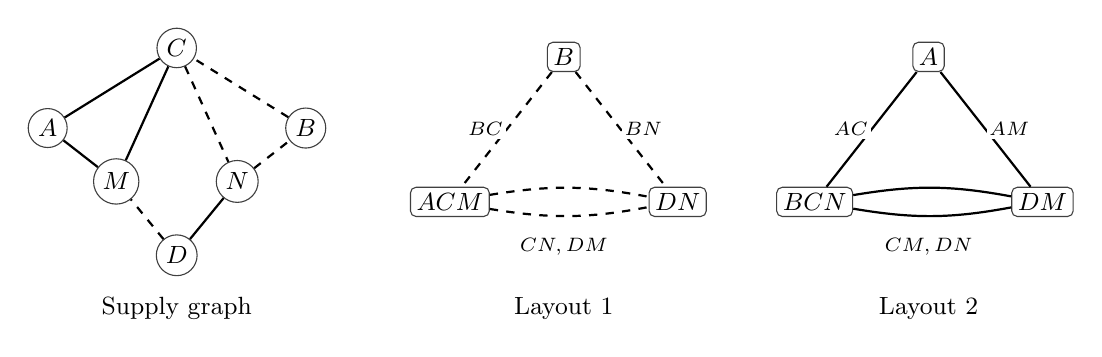
\begin{tikzpicture}[scale=1.13,
 pt/.style={circle,draw=black!75,fill=white,inner sep=1.7pt,font=\small},
 grp/.style={draw=black!75,fill=white,rounded corners=2pt,
              inner sep=2.2pt,font=\small},
 tag/.style={font=\scriptsize,fill=white,inner sep=1pt}]
 \begin{scope}
 \node[pt] (a) at (-1.45,.15) {$A$};
 \node[pt] (b) at (1.45,.15) {$B$};
 \node[pt] (c) at (0,1.05) {$C$};
 \node[pt] (m) at (-.68,-.45) {$M$};
 \node[pt] (n) at (.68,-.45) {$N$};
 \node[pt] (d) at (0,-1.28) {$D$};
 \draw[thick] (a)--(c)--(m)--(a) (d)--(n);
 \draw[thick,dashed] (b)--(c)--(n)--(b) (d)--(m);
 \node at (0,-1.88) {\small Supply graph};
 \end{scope}
 \begin{scope}[xshift=4.35cm]
 \node[grp] (t) at (0,.95) {$B$};
 \node[grp] (l) at (-1.28,-.68) {$ACM$};
 \node[grp] (r) at (1.28,-.68) {$DN$};
 \draw[thick,dashed] (t)--node[tag,left] {$BC$} (l)
                  (t)--node[tag,right] {$BN$} (r)
                  (l) to[bend left=10] (r)
                  (l) to[bend right=10] (r);
 \node[tag] at (0,-1.18) {$CN,DM$};
 \node at (0,-1.88) {\small Layout 1};
 \end{scope}
 \begin{scope}[xshift=8.45cm]
 \node[grp] (t) at (0,.95) {$A$};
 \node[grp] (l) at (-1.28,-.68) {$BCN$};
 \node[grp] (r) at (1.28,-.68) {$DM$};
 \draw[thick] (t)--node[tag,left] {$AC$} (l)
           (t)--node[tag,right] {$AM$} (r)
           (l) to[bend left=10] (r)
           (l) to[bend right=10] (r);
 \node[tag] at (0,-1.18) {$CM,DN$};
 \node at (0,-1.88) {\small Layout 2};
 \end{scope}
\end{tikzpicture}
\caption{Two placements of the supply graph for the demands $AB$ and $CD$.
Layout 1 contracts
the solid edges $G_1$ and retains the dashed edges $G_2$. Layout 2 contracts $G_2$ and retains $G_1$. The two parallel edges
in each layout represent distinct supply wires.}
\label{fig:motif-layout}
\end{figure}

\begin{lemma}[Six-party energy saving]
\label{lem:motif}
Take $t=1/2$ and give $AB$ and $CD$ masses
$r=t^2/(1-t^2)=1/3$ and $1$, respectively. There are rational positive
supply masses, of total $1+r$ in each group, for which
\begin{equation}
 r d_{AB}^2+d_{CD}^2\ \le\ \frac{31}{16}\sum_{e\in G_1\cup G_2}q_e d_e^2
 \label{eq:motif-six}
\end{equation}
holds for every six-point configuration in a $\mathrm{CAT}(0)$ space,
and hence for every assignment in a spectral wire pseudometric over $\mathbb F$.
\end{lemma}

\begin{proof}
Embed the wire distances into a $\operatorname{CAT}(0)$ space by Corollary~\ref{cor:spectral-geodesic} and Lemma~\ref{lem:catzero}. Write $XY$ for the distance between $X$ and $Y$. Give the pairs $(AC,BC)$, $(AM,BN)$, $(CM,CN)$ and $(DM,DN)$ effective coefficients $1/2,1/4,5/6,1$, respectively. Let $E$ be their weighted sum of squared lengths. Put $U=[C,M]_{1/3}$ and $V=[C,N]_{1/3}$. Equation~\eqref{eq:cur-cn} gives
\[
  \tfrac12 AC^2+\tfrac14 AM^2\ge\tfrac34 AU^2+\tfrac16 CM^2
\]
and the corresponding bound with $B,N,V$. Adding the remaining terms leaves $CM^2+CN^2+DM^2+DN^2$ in addition to $\tfrac34(AU^2+BV^2)$. At the midpoint $O$ of $MN$, the midpoint inequality bounds those four squares below by $2CO^2+2DO^2+MN^2\ge CD^2+MN^2$. Hence
\[
 E\ge\tfrac34(AU^2+BV^2)+CD^2+MN^2 .
\]
Convexity along geodesics gives $UV\le MN/3$, so $AB\le AU+BV+MN/3$. Weighted Cauchy--Schwarz gives
\[
 \tfrac13 AB^2\le\tfrac{25}{27}\bigl(\tfrac34(AU^2+BV^2)+MN^2\bigr).
\]
Thus $E$ bounds $\tfrac13 AB^2+CD^2$ from above. The effective coefficients sum to $31/12$ in each layout group. Dividing them by $31/16$ gives the required rational masses, of total $4/3$ per group.
\end{proof}

In the packing used in Section~\ref{sec:compressor}, a bit at each
endpoint marks it thick or thin. A fraction
$t^2=1/4$ of wires have two thick endpoints, and the packing distributes
their total mass over the remaining fraction $3/4$. This fixes $r=1/3$.
Fix any $31/16<H'<2$ in Theorem~\ref{thm:conversion} for this motif.
After choosing one term at each occurrence in a collection of motifs,
one common layout suffices to discard at least half of their total
supply energy. Indeed the surviving costs under the two layouts sum to
the entire supply energy. Before rounding widths to regularize the
degrees, the leading coefficient on the demand energy is therefore
$H'/2<1$. The construction in Section~\ref{sec:compressor} realizes both identifications consistently
when different occurrences share positions and preserves the strict
saving through rounding.
\section{Compression of a wire network}\label{sec:compressor}

Theorem~\ref{thm:compressor} gives an exact expansion of a wire network.
After $T$ blocks, the sum of the surviving widths in each term is
bounded by $2^{-T}$ times a quantity determined by the initial network.
A block has two stages. Several applications of the six-party identity
reduce the leading coefficient of a quadratic energy bound while
increasing the degree. The port graph then restores the original degree
with a multiplicative loss independent of the intermediate degree.
This independence permits iteration.

\subsection{Wire networks and local identities}

Let the base be a finite indexed directed multigraph with distinct endpoints
on every arc and with $d$ incoming and $d$ outgoing arcs at every vertex,
where $d$ is a power of two. Number the slots at each vertex separately in
each direction. Give each base arc $e:x\to y$ a displacement $\tau_e$ in a
binary vector space of lanes. The positions are the pairs $(x,g)$ of base
vertex and lane. The actual arcs over $e$ are
\[
       (x,g)\longrightarrow (y,g+\tau_e).
\]
Directions and slots index the wires. An actual arc of width $b_e$ equates
two strings of $b_e$ bits. The integer width, possibly zero, can vary from one
lane to another. With $P$ positions there are $Pd$ actual arcs. Give each
mass $p=1/(Pd)$ and put
\[
   \mathcal L=\sum_{e\,\text{actual}} b_e^2/p,
   \qquad \sum_{e\,\text{actual}} b_e\le\sqrt{\mathcal L}.
\]
To bound the energy of a concatenated wire, let $p_i$ and $b_i$ be
the masses and widths of its constituents. Cauchy--Schwarz gives
\[
        \frac{(\sum_i b_i)^2}{\sum_i p_i}\le\sum_i b_i^2/p_i.
\]
Thus a concatenated wire can inherit the total mass of its constituents
without increasing energy. Splitting it across integral slots incurs only
the rounding error estimated below.

Write $a_u$ for the string of incident half-wire indices at position $u$,
and $W((a_u)_u)$ for the product of the wire equalities. A substep gives an
identity of the form
\begin{equation}\label{eq:kernel}
 W((a_u)_u)=\sum_{\iota}\ \sum_{z}
   \prod_{v} K_{v,\iota}
       \big((a_u)_{\pi_\iota(u)=v},\,z|_v\big).
\end{equation}
Here $\iota$ is a list of admitted motif terms. The new topology, widths,
placement $\pi_\iota$ of old positions, and kernels are determined by this
list. The variable $z$ chooses one string per new actual arc, used at both
ends. A kernel consists of local ties, sums over local indices, and entries
of the maps in Theorem~\ref{thm:conversion}. After multiplying by arbitrary old
vertex factors and summing the $a_u$, every whole old factor belongs to the new
vertex $\pi_\iota(u)$. In this sum the two old half-wire indices can be
chosen separately, as their former equality has been expanded. Any uncontracted
indices of an old factor move with it. All identities below hold in every
commutative unital ring satisfying the fixed equations on the map entries.

\begin{theorem}[Iterated compression]\label{thm:compressor}
Suppose there are ports over $\mathbb F$ in the sense of
Definition~\ref{def:ports}. Use the family of connected loop-free symmetric regular
graphs of fixed degree and arbitrarily large power-of-two orders from
Section~\ref{sec:ports}. Its squared-distance Poincar\'e bound holds
with one constant for every spectral wire pseudometric over $\mathbb F$.
There exist a
power-of-two degree $d_0$, a positive integer $b_0$, a constant $C_2\ge2$
and finitely many motif templates, all fixed, with the following property.
Let a network of the stated form have $P_0$ positions of degree $d_0$,
maximum width $W_0$, and at least $Tb_0$ lane coordinates, for $T\ge1$.
It has an exact expansion by $T$ blocks of local identities
\eqref{eq:kernel}, ending at degree $d_0$. The same finite system of
parameter equations, satisfiable in $\mathbb F$, suffices for every network and $T$.
For every sequence of admitted terms,
\begin{equation}\label{eq:compress-bound}
  \sum_{e\,\mathrm{final}} b_e\le\sqrt{\mathcal L_T}
  \le 2^{-T}\big(\sqrt{\mathcal L_0}+O(P_0)\big).
\end{equation}
All intermediate wire and kernel fields have length at most
$C_2^T(W_0+1)$. At each final position, the recursive expansion of its
vertex tensor uses at most $C_2^T$ occurrences of vertices, map entries
and fields. This counts each initial factor and each map entry as an
unevaluated operation in the local contraction, with one occurrence
shared by all values of its hidden indices. For fixed arguments, a nonzero map entry contributes
a monomial of parameter degree at most $C_2^T(W_0+1)$.
\end{theorem}

\subsection{Packing the wire slots}\label{sec:compressor-slots}

The lane coordinates let us replicate each base arc in four endpoint
configurations. We mark each endpoint thick or thin. Thick positions
will merge at a fixed site, whereas thin positions can move to either
end of an assigned bundle. The assignment must move every occurrence
of a given old position together, even when several motifs meet there.

\begin{lemma}[Packing and placement of the wire slots]\label{lem:compressor-slots}
For every power-of-two base degree $d$, set $K=2^{2d+1}d$ and $Q=3K/4$.
There is a packing of the wire slots, using a number of lane coordinates
depending only on $d$, with the following properties. The two layouts
refer to the six-party motif of Figure~\ref{fig:motif-layout}.
\begin{enumerate}
\item Packing the thick positions produces $P/K$ new positions. Each
thick--thick bundle contains $K/4$ wires. Every other wire is assigned as
a $CD$ demand to the bundle of its thin $C$ endpoint, with $Q$ per bundle.
\item In either layout the packed endpoints $A,B$ and the image $D^*=\pi(D)$
of the other endpoint have distinct bases in each motif. Each of these three
roles occurs exactly $dQ$ times per new position.
\item Translation of the remaining lane preserves the assignments, placements
and unweighted slots. Slot numbering, including the padding
to any admissible output degree, can be determined by bounded-size lists
per new position after a greedy scan of the base.
\end{enumerate}
\end{lemma}

\begin{proof}
Color the base greedily with $2d+1$ colors. Split the lane as $(U,h,j,g)$,
where $U$ supplies one bit per color, $h$ indexes the $d$ outgoing slots,
$j$ is a tag in a binary vector space of order $J$, and $g$ is the remaining
lane. We determine $J$ below. Call a position thick if its base-color bit
is $1$, and thin otherwise. Put $K=2^{2d+1}d$, the number of pairs $(U,h)$.
Along a base arc the endpoint colors are distinct. With $j,g$ fixed at one
end, the two tests use distinct free bits of $U$ up to translations. They
are independent fair tests, also independently of $h$ at either end.
Consequently each of the four endpoint types occurs $K/4$ times.

For given $x,j,g$ pack all thick positions there into a single new one, with
base $(x,j)$ and lane $g$. There are $P'=P/K$ new positions. Bundle the
$K/4$ thick--thick wires of each base arc for fixed $j,g$ at its source by
concatenating them in a common order at both endpoints. The bundle runs from
a packed position $A$ to a packed position $B$. For every wire outside these
bundles take a thin end for $C$ and the other end for $D$. For thin--thin
wires take their old direction $C\to D$.

Give each base vertex $x$ an offset $\phi_x$. Assign each thin position
$(x,U,h,j,g)$ to the bundle with source $(x,j+\phi_x,g)$ on the outgoing
base arc of slot $h$. Every wire on which this position plays $C$ is assigned
to that bundle. To count these wires, fix the base, tag, remaining lane and
slot of its possible thin sources. The $d$ originally outgoing incidences
contribute $d(K/(2d))=K/2$ wires. The $d$ originally incoming incidences
from thick positions contribute $d(K/(4d))=K/4$. Thus each bundle receives
$Q=3K/4$ wires of type $CD$.

We choose the tag offsets so that $A,B,D^*$ always have distinct new bases.
The old base components of $A,B$ differ. For $C$ at old base $x$ with tag
$j$, and $D$ at $y$ on their old base arc $e$ in either direction, write
\[
          L_x=\{0\}\cup\{\tau_f^{\mathrm{tag}}: f\text{ leaves }x\}.
\]
The new tags of $A,B$ lie in $j+\phi_x+L_x$. A thick $D$ has tag
$j+\tau_e^{\mathrm{tag}}$, and the possible tags of a thin $D^*$ belong to
$j+\tau_e^{\mathrm{tag}}+\phi_y+L_y$. It suffices to impose, at each
incidence,
\[
      \phi_x\notin\tau_e^{\mathrm{tag}}+L_x,
      \qquad \phi_x+\phi_y\notin\tau_e^{\mathrm{tag}}+L_x+L_y.
\]
Greedy choice in base order works for any power of two
$J>2d((d+1)+(d+1)^2)$, since at most this many values are forbidden by
the first conditions and the already assigned neighbors in the second.

\smallskip
At every new position $d$ bundles start and $d$ bundles end, so each of
the roles $A,B$ occurs $dQ$ times. The thick $D$ endpoints at this position
contribute $2dK/4=dK/2$ occurrences of $D^*$, counting mixed arcs in both
old directions. The others are destinations of thin--thin arcs. Before
placement, for fixed base, tag and remaining lane, these contribute $dK/4$
occurrences, equally distributed over destination slot labels $h$. In
layout~1 the tag offset permutes the tags. In layout~2 each position receives
through $d$ incoming base arcs, each with a uniquely determined source tag
and remaining lane, and each carrying $K/4$ such occurrences from its
assigned slot. In both cases the total number of $D^*$ roles is
$dK/2+dK/4=dQ$.

Packing, bundle assignment, and the two choices of image depend on the
remaining lane only through the given arc translations. The common choice
of layout therefore preserves this symmetry. For each surviving occurrence,
label its parallel slots by the original $CD$ arc identifying the motif, the
surviving type, and the subdivision index. When a common deficit remains
after the degree calculation in Subsection~\ref{subsec:shrink}, add zero-width
arcs to the next tag cyclically at the same old base and remaining lane.
Number incoming and outgoing slots separately by sorting their identifiers,
expressing all remaining lanes relative to the vertex being numbered. The
orders transport from lane zero to every lane. Widths and term-dependent map
entries need never enter these identifiers.

Greedy coloring and tag selection each use a single scan of the indexed
base and bounded neighbor lists. After these scans the assignments can be
formed by listing the actual arcs by bundle, and the regularized slots by
their endpoints. The list sizes depend only on the fixed degrees and lane
coordinates consumed in this step. The sorted identifiers give the two
corresponding slot numbers and their displacement, as required for the
next level of the construction.
\end{proof}


\subsection{The energy estimate for one shrinking step}\label{subsec:shrink}

Use the masses of Lemma~\ref{lem:motif}. Write $t=1/2$, $r=1/3$, give the
two demands $AB,CD$ relative masses $r,1$, and give each supply type $e$ its
positive rational relative mass $q_e$. Each of the two supply groups has
total relative mass $1+r$. Fix $31/16<H'<2$ in Theorem~\ref{thm:conversion},
using the metric inequality of Lemma~\ref{lem:motif}, and choose $0<\delta_0<1$ such that
\[
                  \rho=\frac{H'}{2(1-\delta_0)}<1.
\]
With current degree $d$, the step works for every sufficiently large
power of two $d'$ as its output degree. For every term its energy satisfies
\begin{equation}\label{eq:compress-shrink}
        \mathcal L_{\mathrm{new}}\le \rho\mathcal L+O_{d,d'}(P^2).
\end{equation}
The fixed field and motif data may enter all implicit constants.

\paragraph{Packing and assignment.}
Apply Lemma~\ref{lem:compressor-slots}. There are $P'=P/K$ new
positions, with $K=2^{2d+1}d$. Each bundle concatenates $K/4$ thick--thick
wires between the packed endpoints $A,B$. Divide this payload into
$Q=3K/4$ integral pieces as evenly as possible and pair each piece
with one of the $Q$ demands $CD$ assigned to the bundle.

Give these two demands actual masses $rp,p$. Since $rQ=K/4$, the pieces
collectively inherit the mass of the bundled wires. A bundle of total width $b$
would cost $b^2/(Qrp)=b^2/((K/4)p)$ under perfectly equal division. By
Cauchy--Schwarz this is at most the original energy of its thick--thick
wires. Dividing an integer $b$ evenly into $q$ integers raises their sum of
squares above $b^2/q$ by at most $q/4$: their deviations are centered and
the variance of the two consecutive values is at most $1/4$.
Thus rounding costs at most $Q/(4rp)$ per bundle. There are $P'd$ bundles,
and each $CD$ wire keeps its energy. The total demand energy is therefore
at most $\mathcal L+O_d(P^2)$. Apply the wire identity of
Theorem~\ref{thm:conversion} with the masses of Lemma~\ref{lem:motif} to
each motif. After scaling masses by $p$, its additive cost is $O(1/p)$ per motif,
and there are $P'dQ=O_d(P)$ motifs. In every list of terms the total supply
energy is at most $H'\mathcal L+O_d(P^2)$.

\paragraph{Choosing the placement.}
The two layouts send each thin position to opposite ends of its bundle.
Because Equation~\eqref{eq:motif-conversion} is an identity before any
sites are identified, we can select a common layout after choosing the
motif terms.

The first supply group $G_1$ consists of the triangle on $A,C,M$ and the
edge $DN$. The second, $G_2$, consists of the triangle on $B,C,N$ and the
edge $DM$. Choose a single layout for the entire list of terms, retaining the
group of smaller total energy, with deterministic tie breaking. Each layout
first defines the placement $\pi$ of whole old positions. A thick position
goes to its packed site. A thin position goes to the $A$ of its assigned
bundle in layout~1 and to its $B$ in layout~2. This places every $C$ as
required. In every motif the $D$ map goes to $D^*=\pi(D)$, even if that old
position plays $C$ or $D$ elsewhere. Its old vertex factor thus moves only
once.

In layout~1 put the fresh $M$ at $A$ and the fresh $N$ at $D^*$. All edges
of $G_1$ become local. Of the surviving edges, $BC$ joins $B,A$, $BN$ joins
$B,D^*$, and $CN,DM$ join $A,D^*$. Layout~2 interchanges $A,B$ and $M,N$,
making $G_2$ local. The choice retains at most half of the total supply energy.

\paragraph{Regularizing the degree.}
Lemma~\ref{lem:compressor-slots} arranges that $A,B,D^*$ have distinct
bases in each motif and that each of these three roles occurs exactly $dQ$
times at every new position, in either layout.
The new arc mass is $p'=1/(P'd')=pKd/d'$. For every surviving type $e$ use
$m_e=\lfloor p q_e/p'\rfloor$ parallel arcs per occurrence, oriented by its
two roles in a fixed order. Take $d'$ large enough that $m_e>0$ and
$m_e p'\ge(1-\delta_0)p q_e$ for all types. Since each role occurs $dQ$
times, both the in-count and the out-count at every position are
\[
       dQ\sum_{e\,\text{surviving type}}m_e
       \le dQp(1+r)/p'=d'.
\]
Fill the common deficit with zero-width arcs as in
Lemma~\ref{lem:compressor-slots}. The slots commute with translations of the
remaining lane, so the new graph again has fixed displacements on its base
arcs. This symmetry concerns only the unweighted slots. Widths and map
entries may differ on every lane.

Split the surviving payload of width $b$ as evenly as possible among its
$m_e$ slots. The new cost is at most $b^2/(m_ep')+m_e/(4p')$.
The multiplicative loss relative to its supply energy is at most
$1/(1-\delta_0)$. For these fixed degrees there are $O_d(P)$ occurrences,
$m_e$ is bounded, and $1/p'=O_{d,d'}(P)$. Summing this estimate after the
choice of layout proves \eqref{eq:compress-shrink}.

\paragraph{Exact contraction and size of a kernel.}
Concatenating the thick--thick fields and slicing them identically at both
ends rewrites the old wire tensor as the product of the joint $AB,CD$
demands. Expand each with its selected motif identity, summing over lists
of selections. Put the maps for $C,D$ at the images of these old endpoints
and place all other maps by the selected layout. Every absorbed wire is
summed once inside its new position. The remaining wire bits are exactly the
bits allocated to parallel slots. This proves \eqref{eq:kernel}, including
when the layout depends on the term list. A new vertex receives boundedly many
old positions, since the number of slots and consumed coordinates is fixed.
It contains boundedly many maps and wire fields, by the role counts. If the
largest old width is $W$, each new or local field has length $O_{d,d'}(W+1)$,
by the bundle bound and Theorem~\ref{thm:conversion}. Concatenations and
slices are described by bounded lists of field identifiers, offsets and
lengths, even where two slice boundaries differ. Each map needs only the
compact term description and widths from the conversion theorem.
\subsection{Restoring the degree}\label{subsec:refresh}
Let $d_H$ and $\gamma_H$ be the degree and Poincar\'e constant of the
loop-free port graphs constructed in Section~\ref{sec:ports}.

Fix a power of two $d_0\ge \max\{4,d_H+1\}$.
Choose the last shrinking step so that its output degree $D$ is an order in the port family. Use the graph of that order on the $D$ ports. We give a step that
keeps all $P$ positions and returns their in- and out-degrees to $d_0$.
The arc mass changes from $p=1/(PD)$ to $p'=1/(Pd_0)=Dp/d_0$.

Consume $\log_2 D$ lane coordinates as a port index $j$, and include $j$ in
the new base label. For each old base vertex $x$ and remaining lane $g$, its
$D$ ports form one block. An old base arc $e:x\to y$ sends the $D$ ports in a source
block bijectively to those in a single destination block, by translation of both
the port and the remaining lane. Concatenate these $D$ wires, in source-port order,
into one external wire. Its endpoints are the port numbered by the outgoing slot of
$e$ at $x$ and the port numbered by its incoming slot at $y$. Record the same
ordering at the destination. Every port has exactly one outgoing and one incoming
external arc. If the old widths in this bundle were $b_1,\ldots,b_D$, its new
energy is bounded by
\[
 \frac{(\sum_j b_j)^2}{p'}\le \frac{D}{p'}\sum_j b_j^2
     =d_0\sum_j\frac{b_j^2}{p}.
\]

Inside each block, tie every old half-wire to its segment of the external
wire at the designated port. A tie within one port is local. The other ties
form two copies of all ordered pairs of distinct ports, one copy for the
outgoing slots and one for the incoming slots. Each tie has the width of its
old wire and gets mass $p$, so the total internal demand energy over all blocks
is at most $2\mathcal L$. Supply these ties with the directed expander arcs of
the block, each of mass $p'$. The demands test all port pairs, while the
supply tests only expander neighbors. The Poincar\'e inequality compares these
two averages with a constant independent of the number of ports. This is
exactly the metric comparison needed to convert the dense demand into
bounded-degree supply. In detail, for any spectral wire metric $d$ on the ports,
the common Poincar\'e bound gives
\begin{align*}
 \sum_{e\,\text{internal demand}}p\, d_e^2
   &= 2p\sum_{u,v}d(u,v)^2
    \le \frac{2\gamma_H Dp}{d_H}\sum_{e\,\text{expander arc}}d_e^2 \\
   &= \frac{2\gamma_H d_0}{d_H}\sum_{e\,\text{expander arc}}p'\,d_e^2 .
\end{align*}
Apply Theorem~\ref{thm:conversion} to the fixed $D$-port motif with all
masses divided by $p$, and use $H'=2\gamma_Hd_0/d_H+1$.
In each term the internal supply energy increases by a factor at most $H'$
up to an additive $O_D(1/p)$ per block. Summing the external and internal
estimates yields
\begin{equation}\label{eq:compress-refresh}
 \mathcal L_{\mathrm{new}}\le C_*\mathcal L+O_D(P^2),
 \qquad C_*=d_0+2H'.
\end{equation}
In particular $C_*$ is independent of $D$.

The internal identities and the external wires produce the
kernel in Equation~\eqref{eq:kernel}. Before the internal replacements,
summing an external wire with its segment ties restores the old wire equalities.
Each port now has $1+d_H$ arcs in each direction. Pad the deficit with
zero-width arcs from each port to the next in cyclic order. The external
arcs have distinct old base endpoints. Internal and padding arcs have distinct
port endpoints. All slots commute with translations of the remaining lane.
One old position stays at each new position, the number of local maps and
fields there is bounded in terms of $D$, and their lengths are
$O_D(W+1)$ when the incoming maximum width is $W$.

\subsection{Iteration}

\begin{proof}[Proof of Theorem~\ref{thm:compressor}]
Choose a positive integer $s_0$ so that $C_*\rho^{s_0}\le1/4$. Starting
from $d_0$, choose in succession $s_0$ sufficiently large power-of-two
output degrees for the shrinking steps. Choose the last to be an expander
order $D$ from this family, then restore the degree to
$d_0$. This order of choices is possible because $\rho$ and $C_*$ are
independent of the chosen degrees. The resulting block uses a fixed
number $b_0$ of lane coordinates. Each of its finitely many templates has
equations solvable in $\mathbb F$. Use disjoint names for their parameters and take
the union of the equations.

Every shrinking step divides the position count by its own $K$, while the
refresh preserves the count. Write $\kappa_0>2$ for the product of these
fixed $K$'s in a block. At the start of block $i$, numbered from zero,
there are $P_i=P_0/\kappa_0^i$ positions. Composing
\eqref{eq:compress-shrink} and \eqref{eq:compress-refresh} within a block
gives a fixed $c$ with
\[
          \mathcal L_{i+1}\le\tfrac14\mathcal L_i+cP_i^2 .
\]
Consequently
\[
   \mathcal L_T\le 4^{-T}
     \left(\mathcal L_0+4cP_0^2
                \sum_{i=0}^{T-1}(4/\kappa_0^2)^i\right).
\]
The geometric sum is uniformly bounded, giving \eqref{eq:compress-bound}.

At each of the fixed substeps a bound on the incoming field lengths changes
from $W$ to at most a constant times $W+1$, including the internal fields.
At each new position the numbers of immediate preimages, maps and field
descriptions are bounded by a constant. Iterating these two estimates down
the tree of local contractions gives the two bounds with $C_2$ sufficiently
large. This constant may also absorb a fixed number of description items per
occurrence and the constant in the linear bound on the degree of a map entry
from Theorem~\ref{thm:conversion}. Once final arc bits and term choices
are fixed, each final vertex sums only its own hidden indices, because each
substep sends each entire old vertex to one new position.
\end{proof}

\subsection{Computing the local contraction records}\label{app:descriptors}

The width estimate controls the summands in the expansion. To implement
their sum, we must also recover the contractions specified by a sequence
of terms. A \emph{descriptor} records the offset and length of a bit
field, together with the map or old vertex that uses it. These records
can be constructed before assigning any wire bits.

\begin{lemma}[Compressor descriptors]\label{lem:descriptors}
Under the hypotheses of Theorem~\ref{thm:compressor}, suppose that
$n\ge P=P_0$, $W_0\le n^{O(1)}$, and $T=O(\log n)$. There is a
nondeterministic RAM procedure with $O(\log n)$-bit words that takes
the initial slot records and widths as input. Its successful paths are
in bijection with the sequences of admissible term indices in the
theorem. Each such path constructs the following records at every level.
\begin{enumerate}
\item Each actual incident slot gives access to its arc width and both
endpoint slots. The base slots specify lane displacements.
\item Each new position has its full list of immediate old positions,
its local maps and their term data, and the slices, ties and summed fields
needed to evaluate its kernel in Equation~\eqref{eq:kernel}. Each position
has boundedly many records, accessible by their addresses.
\end{enumerate}
The procedure takes $O(P\operatorname{polylog} n)$ steps. With
comparisons, bit operations, shifts and ordinary word arithmetic, the
polylogarithmic exponent can be taken to be an absolute constant
(for instance, ten).
\end{lemma}

\begin{proof}
Store the lemma's records in arrays indexed by level, slot and position.
To reconstruct a map argument, identify each field by its source, offset
and length. For instance, when
concatenated fields are repartitioned, intersect the two lists of
intervals in the concatenation to obtain the slices to copy. Each local
map description contains its motif, role, fixed template, demand widths,
and the term index, including the numerical data for checking the total
payload widths on \emph{all} edges of that motif. At this stage a map
entry is represented by this description, without writing out the
selectors or the bit positions of its copies.

All degrees and templates in one compressor block are fixed. Theorem~\ref{thm:compressor}
bounds the number of immediate preimages, fields and maps per position
by a constant for each substep. Thus each position needs only a bounded
number of records per level. A record uses a bounded number of words.
Levels, slots, base vertices, tags and lanes admit direct product indexing
with $O(\log n)$ bits per index, since the numbers of sites and levels
are polynomial in $n$. Arrays for successive levels can occupy disjoint
address ranges. Blank space needs no initialization. 

To implement the slots and placements of Lemma~\ref{lem:compressor-slots},
a shrinking substep uses three scans.
\begin{enumerate}
\item In base order, compute the greedy colors and tag offsets. Looking
up a base vertex's neighbors, their incident displacements and earlier
assignments takes boundedly many accesses. Identify a bundle by its base
arc, source tag and remaining lane, and a motif by its $CD$ arc. Scan the
actual arcs, appending each thick--thick arc and each $CD$ arc to the
appropriate lists. Record the packing of every thick position and both
possible placements of each thin position. Order the bounded lists using
identifiers in which lane coordinates are written relative to the bundle's
source lane (by xor). This fixes the order consistently under translation
of the remaining lane. Divide each bundle into the prescribed pieces and
record their slices at both ends.
\item In a fixed order guess one term index per motif, using fixed-length
binary encodings and rejecting out-of-range or inadmissible indices. Each
admitted index occurs once, including indices whose terms may eventually
contribute zero. Accumulate the two possible surviving energies while
scanning, then choose the common layout with the prescribed tie rule. The
common mass factor cancels in this comparison. The other coefficients are
fixed rationals, and the scores are sums of polynomially many squared
integer widths of polynomial magnitude. The numerators and denominators
therefore use $O(\log n)$ bits after clearing a fixed denominator.
The grid, payload and rounding tests for an index likewise use fixed
rational tables and integer comparisons.
\item Store the chosen layout once for the level. Scan old positions,
appending each position exactly once to the preimage list at its selected
destination. For a thin position this takes the recorded endpoint of
its one assigned bundle, even when the position carries roles in several
motifs. Record each role incidence separately at this same destination.
Generate the surviving slots for each motif together with
endpoints, role edge and subdivision number. Include zero-width slots and
generate the prescribed dummy slots. At each position order the outgoing
and incoming slots separately by origin, using the motif's identity
relative to that position's lane, its role edge and subdivision number,
or the dummy slot's identity. These keys use only the combinatorial
placement in the chosen layout. In particular they are independent of
payload widths. Give each generated actual arc its own record indexed
by its absolute motif ID, role edge and subdivision number (or its dummy
ID). Both endpoint lists carry that address. After each bounded list is
sorted, write its local slot number back to the corresponding endpoint
field in the arc record. A scan of the outgoing slots at lane zero can
now read the destination slot and xor displacement directly. Since
translation preserves the relative keys, these are the base records for
every lane. The individual widths and term indices stay in the actual
records. Split surviving widths as prescribed.
Record the argument slices for the maps, the internal identifications of
absorbed supplies and the slices occupying the new incident arcs.
\end{enumerate}
For a degree refresh the port blocks have fixed size $D$. For each old
base arc and source block, list its $D$ actual arcs in source-port order,
using the known translated port at the other end. This describes both
ends of the concatenated external arc. In each block guess one internal
motif term as above and record its demand, supply and map arguments.
The new incoming and outgoing lists each have one external slot. Reserve
the other slots for the indicated internal and dummy arcs. These direct
correspondences specify the slices and ties at every port.

Each scan visits $O(P)$ records, since the number of positions never
increases. Each visit needs at most polylogarithmically many elementary
operations and probes. There are $O(\log n)$ substeps, so the entire
descriptor phase costs $O(P\operatorname{polylog} n)$. In particular this phase pays for numerical widths
through their binary lengths.
\end{proof}

\section{Exact descent with tagged-permutation gates}\label{sec:exact}

In Theorem~\ref{thm:compressor}, each summand uses few wire bits. The
available slots may nevertheless occupy a large network, and the local
contractions still have to be evaluated. We realize the full sum in
one network by compressing a batch of copies together. Copies share
the cost of specifying the wiring, and short descriptions of the local
contractions permit simultaneous table lookup. The only gates of
unbounded arity are tagged-permutation tests of a single length.

Call a trivalent network \emph{normalized} if it has no self-loops and
each open bit is carried by a separate equality leaf adjacent to an
interior vertex. Inserting equality leaves and subdividing self-loops
changes the size by at most a constant factor.

\begin{proposition}[Descent with tagged-permutation gates]
\label{prop:oracle-descent}
Let the finite field have ports in the sense of Definition~\ref{def:ports}.
There is an $a\in(0,1)$ with the following property. Fix $J\ge 2$.
For every sufficiently large $h$, put $N=2^h$, let $N\le m\le N^J$,
and let $G$ be
a normalized trivalent network of size at most $m$ with $e$ open bits.
There is a positive integer $d$ with $\log_2 d=O((\log h)^2)$ and an
exact network for $G^{\otimes d}$ of size
\[
                      O\bigl(d(m/h^a+e\operatorname{polylog} h)\bigr)
\]
whose gates are trivalent except for calls to $\operatorname{Tag}(h,h)$.
The size charges every incident bit wire, including those at calls.
The bounds are uniform in $m$ and $G$.
\end{proposition}

\subsection{Length lifting}
The following version of the column-sorting construction of
Leighton~\cite{Leighton} records the total number of short sorts as
well as their depth.
\begin{lemma}[Lifting the length of a sort]\label{lem:sort-lift}
Let $b\ge 16$ be a power of two. A sort of length $l\ge b$ can
be carried out by layers of independent sorts on $b$ records,
interspersed with fixed permutations, insertions of sentinels, and
deletions of padding. For an absolute $C$, with
$u=1+\log(l)/\log b$, there are at most $C u^C$ layers, using altogether
at most $C(l/b)u^C$ sorts of length $b$. For stability it suffices to
carry the original position through the layers.
\end{lemma}

\begin{proof}
Pad to a power of two $L\in[l,2l)$. First suppose $L=kb'$,
with $b'$ and $k$ powers of two and $k^2\le b'/2$. Arrange $k$
columns of height $b'$. Sort each column. Deal its sorted entries
cyclically into the $k$ new columns and concatenate the contributions
within each new column. Each destination receives $b'/k$ entries from
each source. Sort the new columns and list them in row-major order.
For any cut in the total order, the counts of elements below the cut
in any two new columns differ by at most $k$, since the counts from
each source differ by at most one. In row-major order the binary
string indicating membership below the cut thus has a prefix of ones
and a suffix of zeros separated by a window of at most $k^2$ bits.

Sort aligned blocks of $b'$ consecutive positions, then blocks shifted
by $b'/2$, handling the end half-blocks by padding. A window inside
an aligned block is resolved in the first pass. A window crossing an
aligned boundary is contained in the shifted block centered on that
boundary. Sorting the aligned blocks leaves the already ordered prefix
and suffix outside the window intact, so the second pass resolves the
cut. This holds for every cut. The four passes consequently sort the
list. Each pass uses at most $2L/b'$ calls, a bound allowing for the
two end blocks.

Starting from $b_0=b$, set $b_{i+1}=2^{\lfloor(5/4)\log b_i\rfloor}$.
For $b_i\ge16$ these powers increase, and their logarithms grow at
least geometrically (with ratio at least $8/7$, for example).
Whenever $b_i<L\le b_{i+1}$ we may take $b'=b_i$ in the preceding
construction. At each recursion take the largest $b_i$ strictly below the current
length as the child length, and pad only the end half-blocks.
There are $O(1+\log u)$ levels. The number of sequential passes
increases by a factor at most four per level and their combined padded
record volume by a factor at most eight. At the bottom each full call
uses $b$ record slots. These bounds give the stated constants. Appending
the original position once orders all genuine records distinctly. A
flag distinguishes sentinels and permits their deletion, including
in intermediate calls.
\end{proof}

Apply Lemma~\ref{lem:sort-lift} with base length $b=N=2^h$.
A stable sort of $N$ records of $O(h)$ bits costs $O(Nh)$ using
$\operatorname{Tag}(h,h)$ gates and charging their incident wires
(Section~\ref{sec:width}). If a payload exceeds $h$ bits, split it into a bounded number of
fields and use the same tags for all fields. For $l<N$ pad to
$N$. For $N\le l\le N^{O(1)}$ the ratio $\log l/\log N$ is bounded,
so a stable sort costs $O((l+N)h)$ throughout this range. This bound
also gives simultaneous lookup when $l$ counts the query and
dictionary records together. Sort by key, placing the unique
dictionary record first in each group. Scan the group to answer its
queries, then return the answers in their original order by a second
sort. Each valid input and output has a unique witness.

\subsection{Realizing the compressed expansion}

\begin{proof}[Proof of Proposition~\ref{prop:oracle-descent}]
A compressed bit has two uses. At its vertex it is part of the
argument to a local factor. On its arc it must agree with the bit
at the other endpoint. Vertex lookup requires short keys, since the
table size grows exponentially in the key length. Arc comparison
uses addresses of $\Theta(h)$ bits, so each comparison should cover
a long string. We stack the copies of $G$ to obtain both orderings
within the wire budget.

\paragraph{Stacking the copies.}
Let $d_0\ge4$ be the degree in Theorem~\ref{thm:compressor}. Give each
internal edge of $G$ an arc in both directions, with the wire on just
one arc. Copy this loop-free topology with all widths zero, no
exterior indices, and scalar factor one at each duplicate vertex. Each
vertex and its duplicate have the same in- and out-degree, so we can give
both degree $d_0$ by adding zero-width arcs in both directions between
them. Keep the exterior bits as free indices of their original vertices.

Take $s=\lceil 2a\log h\rceil$ compressor blocks, consuming $b_0 s$
lane coordinates. We choose the constant $a>0$ below. Set
\[
 L=2^{b_0s},\qquad B=\lceil h^{1/2}\rceil,\qquad
 R=2^{\lceil4\log h\rceil},\qquad d=B L R .
\]
Since $b_0$ is fixed, $d=h^{O(1)}$. Use $LR$ lanes with zero initial
displacements and reserve the $\log_2 R$ replication coordinates
throughout. Each lane starts with a tensor product of $B$ copies of
$G$, with $B$ bits per nonempty arc. Put $P=mLR$. There are $O(P)$
initial positions, the maximum width is $B$, and the square root of
the energy is $O(PB)$. Hence Theorem~\ref{thm:compressor} bounds the
total internal wire width in each term of the final expansion by
$O(dm/h^{2a})$.

One binary choice per shrinking substep specifies the \emph{layout
pattern}. Its $O(s)$ bits determine every unweighted topology and
placement in the sequence. Each substep translates by previous arc
displacements or moves locally on the remaining lanes, so the
replication coordinates still have zero displacement. The final graph
therefore consists of $R$ copies of the same set of positions, which
we call \emph{hosts}. Widths and tensors can vary across copies. For
each exterior bit position of $G$ and each lane in $[L]$, the layout
pattern fixes a single host carrying one exterior port of width $B$
per replica. At most $2^{O(s)}$ such ports reach one host, since each
substep merges a bounded number of positions.

\paragraph{Encoding the local contractions.}
For each host and replica we record two kinds of data.
\begin{itemize}
\item The \emph{operands} are the bits in its incident slots and exterior
ports. Their total length is at most $2^{O(s)}B$ by
Theorem~\ref{thm:compressor}.
\item The \emph{program key} describes the factor to evaluate on the
operands and gives the length of each field. Unfold the contraction
records of Lemma~\ref{lem:descriptors} using local names for the
constituent objects. The key lists field offsets, incidence ordinals,
widths, ties, motif templates and term indices. Each leaf carries one
label for the original trivalent factor over the fixed finite field,
which determines its $B$-fold product. Lengths and term indices use
$O(\log h)$ bits apiece, giving $2^{O(s)}\operatorname{polylog} h$
bits for the key.
\end{itemize}

Boolean circuits construct the keys from guesses for the motif terms.
To count each history exactly once, select one layout pattern, check
all its guesses, and set the guesses for the other patterns to zero.
Use a circuit template for each pattern with the graph sequence, greedy
colors, offsets and slot lists hardwired. The only global calculations
are the sums of energies that verify the layout choices. After removing
the common mass factor, all terms have a fixed denominator and
$O(\log h)$-bit numerators. Balanced addition costs
$O(P\operatorname{polylog} h+h)$ per sum, as the word length grows by
one bit per level. Apply the prescribed tie rule.

The width calculations, term checks and slice intersections at one
position use a bounded number of operations on quantities of
polynomial size in $h$. By Theorem~\ref{thm:conversion}, their cost is
$\operatorname{polylog} h$ bits and gates. Fixed wires supply the
local data from preceding steps. Gathering the $2^{O(s)}$ records for
a final kernel, checking for rejection, and copying the selected
outputs over all patterns costs $P\,2^{O(s)}\operatorname{polylog} h$.
A long name, such as an exterior port identifier, is read once per
host slot and shared over all replicas. For fixed $J$ the names use
$O(h)$ bits. Selecting them from the hardwired lists costs an additional
$(P/R)\,2^{O(s)}O(h)$.

Fix $a<0.02$ small enough that all preceding
$2^{O(s)}\operatorname{polylog} h$ bounds are $O(h^{.1})$.
A fixed-format array of program keys takes $O(Rh^{.1})$ bits per host,
including padding for the largest topology. Use base order within each
pattern and pad to $O(P/R)$ hosts, with blank keys encoding unit
factors. Each key gives the operand lengths in local slot order,
including the exterior ports.

\paragraph{Matching the wires.}
Use rows of $h$ bits. For each incident slot at a host, concatenate its
operand bits in replica order to form a stream. An internal stream
must equal the stream at the other end of its arc. An exterior stream
of $BR$ bits must equal the corresponding input bits, which are ordered
by their fixed names for every layout pattern. For each host reserve
control rows for the program keys, stream identifiers, flags and
padding. These occupy $O(R h^{.1}+h^{1.1})$ bits. Reserve whole rows
for each stream, padding its final row after combining its replicas.

The total allocated bit count is
\[
 O\big(P h^{.1}+(P/R) h^{1.1}+d(m/h^{2a}+e)\big)
   =O(S_*),\qquad S_*=d(m/h^{2a}+e).
\]
Each allocation needs at most $O(Rh^{.6}+h^{1.1})$ bits even counting operand bits.

Pack the host allocations in order into bins of $h^8$ rows, starting
a new bin when the next host does not fit. Each host uses at most half a
bin, so a fixed pool of $O(S_*/h+h^8)$ rows suffices. Computing the
allocation lengths costs $O(P h^{.1}\operatorname{polylog} h)$ by
summing the stream sizes given in the keys. Each such local size is
polynomial in $h$.

Scanning the hosts to assign their bins costs $O(h)$ per host for the
bin index and occupancy. Sort the control rows into their prescribed
positions, mark each host's start, and assign a blank control flag to
the remaining rows. An absolute row address uses $O(h)$ bits and can
be updated in linear work by concatenating the bin and offset fields.
The scatter costs $O(S_*+Nh)=O(S_*)$, since $m\ge N$, $R\ge h^4$
and $S_*\ge BLR\,m/h^{2a}$. Sum over guesses for
the stream rows, requiring zeros in all padding and outside the
streams. Parse each allocation deterministically from its controls.
A stream row receives its matching name, side and ordinal, copying
the common prefix from its stream header. One sort and scan verifies
the equality of every pair of internal streams and matches the
exterior streams with fixed input rows. The latter can be rounded to
whole rows per exterior stream within the same $O(S_*/h)$ row budget.

\paragraph{Evaluating the vertex factors.}
For each host and replica, join its program key and operand bits in
operand order into one self-delimiting record. Reserve a length field
in the key and fix the encoding of empty padding. Each record has
$O(h^{.6})$ bits and fits into a row of $\lfloor h/2\rfloor$ bits for
large $h$. Within each bin the sum of record lengths is at most a
constant times the bin capacity. Pack records in order, beginning a
new row when the next record does not fit and padding unused bits
uniquely. A fixed array of $O(h^8)$ rows per bin suffices.

A bit RAM with $O(\log h)$-bit addresses performs these local operations
in at most the bin capacity times $\operatorname{polylog} h$ steps.
It scans the controls, checks padding, and maintains a current offset
for each stream to copy the fields into replica order. Copying the
long headers bitwise costs $O(h)$ transfers per row. As in
Lemma~\ref{lem:tag-amplification}, bitonic sorting of time-stamped
memory records together with local instruction checks verifies the
deterministic trace by a trivalent network. The overhead is
$\operatorname{polylog} h$ since the bin size is polynomial in $h$.

Each packed row specifies the product of the vertex factors in its
records, with value one for an empty row. The fixed finite field and
the local contractions determine a table of at most $\sqrt N$ entries
with constant-sized outputs. Hardwire this table and perform
simultaneous lookup with one scalar factor per request. The cost
is $O(S_*)$, including the table, since all lists have length
polynomial in $N$ for fixed $J$.

Fix the selector bits and exterior indices. The surviving stream
assignments are in bijection with assignments of the final wire bits.
Every deterministic check has a unique valid completion or is used
as its exact relation tensor. Summing the products of the returned
scalars over these assignments and over the selectors gives
$G^{\otimes d}$. The total size is $O(S_*\operatorname{polylog} h)$.
For fixed $a>0$, the factor $h^{-2a}\operatorname{polylog} h$ in the
interior cost is $O(h^{-a})$, as claimed.
\end{proof}

\section{From tagged permutations to amortized simulation}
\label{sec:descent}

Fix a finite field $F$ with largest spectral flat dimension $k$. A
\emph{tick} is a trivalent bit network and its \emph{pins} are its open
data bits. For a tick of size at most $V$, we can reduce the size per
copy to $V/(\log_2 V)^A$ for any fixed $A$, provided the tick has
sufficiently few pins. Each copy retains its own pins. The approximation
must work for every joint choice of their values.

\begin{theorem}[Amortized simulation]
\label{thm:collapse}
For every sufficiently large fixed integer $A$ there is a constant
integer $A'>A$ with the following property. Let $V=2^w$. For all
sufficiently large integers $w$, let a tick have size at most $V$ and
at most $V/w^{A'}$ pins. For some positive integer $q\le V^{o(1)}$,
there is a trivalent network of size at most $qV/w^A$ approximating
the product of $q$ copies of the tick, with gap at least $V^{1-o(1)}$
pointwise in their separate pins. Both asymptotic envelopes are
uniform in the tick.
\end{theorem}

Two costs determine whether the saving can be iterated.
Proposition~\ref{prop:oracle-descent} reduces the size per tick by a
power of the address length, using exact tagged-permutation gates.
Theorem~\ref{thm:cheaptag} replaces those gates at a smaller overhead,
but each replacement exposes new catalyst bits. At the next descent
step every exposed bit counts toward the compiler's boundary cost. We
control that cost by placing copies on a grid and passing each
catalyst wire successively through the cells of a coordinate line.
Only the two ends of the line remain exposed. The price estimate below
quantifies how much of the original gap this operation preserves.

\subsection{Pricing error on a grid}

Consider the grid $\{3,6,\ldots,3g\}^k$. For direction $j$, place
two \emph{foci} at $\pm Re_j$, with $R\ge8g$. There are $E$ external
pairs of bits, each assigned a direction and having one end at each
focus of that direction. In a fixed wiring, choose a grid line in the
assigned direction for each pair. Its \emph{rail} runs from the
negative focus to the first cell on the line, visits its cells in order
and ends at the positive focus.

At each cell the exact wiring uses one factor $f\otimes I_X$. Attach
each of its catalyst pairs to a distinct rail passage in the prescribed
direction. The minus and plus catalyst ports form the incoming and
outgoing ends of that passage. All other passages and the data ports
may participate in an arbitrary local contraction. The rails supply all
intercell connections, and their endpoints at the foci are the only
outputs. The approximate wiring replaces the factor at every cell by
$X$ with gap at least $D>0$. Its data are exposed except for pointwise
pins, whose values must be fixed. We allow both constructions to be
summed over the same collection of at most $2^\ell$ choices of wiring,
local factors and settings.

\begin{lemma}[Lens estimate]\label{lem:lens}
The difference of the two sums has price at most
\[
  2RE-D+O_k(Eg^2/R)+2kR(\ell+g^k).
\]
More precisely, putting $L=g^k$ and taking $c$ to be the binary diagonal
price on the set of all $2k$ foci, it has price at most
\begin{equation}\label{eq:lens-binomial}
  2RE+C_k Eg^2/R+c\ell+
       c\log_2\big((1+2^{-D/c})^L-1\big)
\end{equation}
for a constant $C_k$ depending only on $k$.
\end{lemma}

\begin{proof}
Expand the difference for one wiring by multilinearity. Each term has
a nonempty set of cells at which it uses $X-f\otimes I_X$. At cell $x$,
place the incoming and outgoing ends of a direction-$j$ passage at
$x-e_j$ and $x+e_j$, and the data operations at $x$. Allow two units of
price per passage. This pays for the through identity on a catalyst pair
or, on another passage, for moving both ends to $x$. A cell error saves $D$ from the total allowance at that
cell by \eqref{eq:catalyst-gap} in the translated frame. An interior link
along a rail has length $3-2=1$. Each of its two end links has a longitudinal
component $a\ge R/2$ and perpendicular displacement $u$ with
$\|u\|^2\le 9(k-1)g^2$. Its excess length is
\[
   \sqrt{a^2+\|u\|^2}-a
      =\frac{\|u\|^2}{\sqrt{a^2+\|u\|^2}+a}
      \le \frac{\|u\|^2}{2a}.
\]
The longitudinal parts telescope, including the passage allowances, to $2R$
per rail (Figure~\ref{fig:spectral-lens}). A summand with $i$ erroneous
cells therefore has price at most $2RE+C_kEg^2/R-iD$.

There are at most $2^\ell\binom{L}{i}$ terms of this kind.
Equation~\eqref{eq:price-ordinary-sum} gives \eqref{eq:lens-binomial} by
summing these spectral values. Simply bounding the number of terms by
$2^{\ell+L}$ and using $i\ge1$, with $c\le2kR$, gives the first assertion.
The same output frame is used for every wiring, even when each selector sends
the external pairs to different grid lines.
\end{proof}

\begin{figure}[tbp]
\centering
\begin{tikzpicture}[scale=.9,line cap=round,line join=round,font=\small]
  \definecolor{lensfirst}{RGB}{27,91,130}
  \definecolor{lenssecond}{RGB}{165,72,32}
  \draw[gray!38,dashed] (-3.55,0)--(3.55,0);
  \draw[gray!38,dashed] (0,-3.55)--(0,3.55);
  \foreach \v in {.44,.88,1.32}{
     \draw[gray!40] (.44,\v)--(1.32,\v);
     \draw[gray!40] (\v,.44)--(\v,1.32);
  }
  \draw[lensfirst!55,densely dotted] (1.32,.88)--(1.32,0)
       node[midway,right,font=\scriptsize,text=black] {$\|u\|$};
  \node[below,font=\scriptsize] at (2.43,0) {$a$};
  \draw[lensfirst,thick] (-3.55,0)--(.44,.88)--(1.32,.88)--(3.55,0);
  \draw[lenssecond,thick,dashed] (0,-3.55)--(.88,.44)--(.88,1.32)--(0,3.55);
  \foreach \x in {.44,.88,1.32}{
    \foreach \y in {.44,.88,1.32}{
      \fill[black] (\x,\y) circle (1.45pt);
    }
  }
  \draw[black,fill=white] (.88,.88) circle (2.5pt);
  \fill[lensfirst] (-3.55,0) circle (2pt) node[left] {$-Re_1$};
  \fill[lensfirst] (3.55,0) circle (2pt) node[right] {$Re_1$};
  \fill[lenssecond] (0,-3.55) circle (2pt) node[right] {$-Re_2$};
  \fill[lenssecond] (0,3.55) circle (2pt) node[right] {$Re_2$};
  \begin{scope}[shift={(7.65,.3)}]
    \draw[black!45,rounded corners] (-2.78,-2.12) rectangle (2.78,2.02);
    \draw[lensfirst,thick] (-1.18,0)--(1.18,0);
    \draw[lenssecond,thick,dashed] (0,-1.18)--(0,1.18);
    \fill[lensfirst] (-1.18,0) circle (2pt) node[left] {$x-e_1$};
    \fill[lensfirst] (1.18,0) circle (2pt) node[right] {$x+e_1$};
    \fill[lenssecond] (0,1.18) circle (2pt) node[above] {$x+e_2$};
    \fill[lenssecond] (0,-1.18) circle (2pt) node[below] {$x-e_2$};
    \draw[fill=white] (0,0) circle (2.5pt) node[above right] {$x$};
    \node at (0,-2.56) {$H(X-f\otimes I_X)\le 2(b_1+b_2)-D$};
  \end{scope}
\end{tikzpicture}
\caption{Two rails on a planar grid. At the circled cell each rail uses
the ordered pair of sites shown at right. Its projection from focus to focus
has length $2R$. Only the sloping end links add excess length. The marked
link has length $\sqrt{a^2+\|u\|^2}$ and contributes at most
$\|u\|^2/(2a)$ beyond its projection.}
\label{fig:spectral-lens}
\end{figure}

Splicing a line of $g$ copies reduces its number of external catalyst
pairs by a factor $g$. To transfer this construction back to unit frames,
choose the foci far enough away that the total excess rail length is
small compared with the gap.

\begin{lemma}[Grid reuse]\label{lem:reuse}
Suppose a scalar network at fixed pins has gap at least $D=V^{1-o(1)}$ and
uses $B\le V^{1+o(1)}$ catalyst pairs. Put $g=V^{o(1)}$, a positive
integer. Take $g^k$ copies with separate pins and splice consecutive
catalyst ports on each line in their common direction. The resulting
network approximates the product pointwise with gap $V^{1-o(1)}$ and has
$g^{k-1}B$ external catalyst pairs.
\end{lemma}
\begin{proof}
In each direction there are $g^{k-1}$ grid lines. After fixing the pins
the target is the product of the scalar values times the identity on the
$E=g^{k-1}B$ remaining pairs. Take $D\le V$ by decreasing the claimed
gap if necessary. With $\ell=0$, choose $R=V^{o(1)}$, $R\ge8g$, so that
$Eg^2/R=o(D)$. This is possible since $Eg^2/D\le V^{o(1)}$, and such
an $R$ still gives $Rg^k=o(D)$. For any prescribed unit output frame with
placement $i:\mathbb R^k\to\mathcal X$, use the spectral space with prices
and distances multiplied by $R$ and the isometry $u\mapsto i(u/R)$ into
that rescaled space. The lens foci are now exactly $i(\pm e_j)$.
Lemma~\ref{lem:lens} gives an error price at most $2RE-D/2$ there.
Dividing by $R$ returns to the prescribed frame with gap at least
$D/(2R)=V^{1-o(1)}$. Bounds uniform in the original networks can use a
common choice of $R$.
\end{proof}

\subsection{Iteration of the descent step}

\begin{proof}[Proof of Theorem~\ref{thm:collapse}]
Take $a\in(0,1)$ from Proposition~\ref{prop:oracle-descent}. Apply
Theorem~\ref{thm:cheaptag} with $r=a/4$, so its network for
$\operatorname{Tag}(h,h)$ has size $O(2^h h^{1+r})$ and exposed gap
at least $2^{h-C\sqrt h}$ for a fixed $C$. Choose
\[
 b=a/2,\qquad L=\lceil A/b\rceil,\qquad
 A'=\lceil bL+4\rceil,\qquad
 h=w-\lceil A'\log_2 w\rceil,\qquad N=2^h .
\]
Thus $h\sim w$ and $V/(2w^{A'})\le N\le V/w^{A'}$.

After $i$ steps we shall have a network $G_i$ representing $q_i$ ticks
pointwise with gap $V^{1-o(1)}$ or better. Its size per tick is at most
$V/w^{bi}$, and its total number of open bits per tick, including the
two ends of every catalyst pair, is at most $2V/w^{A'}$.
We also require $q_i\le V^{o(1)}$. The tick itself satisfies these
conditions at $i=0$ with $q_0=1$ and zero error.

Suppose $i<L$. First compile the product using exact tagged gates.
Normalize $G_i$, write $e$ for its open bit count, and
let $m$ be the larger of its normalized size and $N$. Then
$m\le N^2$ for large $w$, since $q_i V=V^{1+o(1)}$ and
$N=V^{1-o(1)}$. Proposition~\ref{prop:oracle-descent} gives an exact
network for $G_i^{\otimes d}$ with
$d=2^{O((\log h)^2)}$. Its size is $V^{1+o(1)}$. The number of tag
calls is $V^{o(1)}$, since each has $3Nh$ bit incidences and each
wire contributes at most two incidences to this count. Replace every
call by the approximation above, retaining all of its catalyst ports.

First apply Lemma~\ref{lem:substitution} to $d$ copies of $G_i$ in
the product of $dq_i$ ticks, with the original pins fixed.
The resulting error bound depends only on the tensor, hence applies
to the exact oracle realization. Apply the lemma a second time to its
tag calls, with their data exposed so that the internal indices may be
contracted. The two applications each lose at most $V^{o(1)}$ in
absolute gap to summation over error terms. The tag gaps
$N2^{-C\sqrt h}$ and the inherited gap are at least $V^{1-o(1)}$.
Thus the result still has gap at least $V^{1-o(1)}$ pointwise in all
$dq_i$ copies' pins.

The compiler charges every bit incident to a tag call. Replacing the
calls therefore increases size by a factor of at most $O(h^r)$.
The compiler's interior cost and boundary cost give, respectively, the
two terms in the following bound on size per tick.
\[
 O\left(\frac{V}{w^{bi+a-r}}+
         \frac{V\operatorname{polylog} w}{w^{A'-r}}\right)
              \le \frac{V}{w^{b(i+1)}}
\]
for sufficiently large $w$. Indeed normalization costs a constant
factor, the floor $m\ge N$ contributes at most the second term, and
$e/q_i\le 2V/w^{A'}$. The two exponents have slack because
$a-r>b$ and $A'-r>bL$.

The new catalyst ports can outnumber the original pins. Apply
Lemma~\ref{lem:reuse} to a grid of side $g=\lceil w^{A'}\rceil$.
Replication by $g^k$ and splicing along the lines in each catalyst
direction preserves the pointwise gap $V^{1-o(1)}$. Indeed the number
of pairs before reuse is at most the total network size
$V^{1+o(1)}$, and $g=V^{o(1)}$. Each line has $g$ copies and keeps
one pair of ends in place of $g$ such pairs. Hence the number of open
catalyst bits per tick falls by a factor $g$, and is now at most
$V/g$. The number of pins per tick is still at most $V/w^{A'}$.
Splicing does not increase the size per tick. This proves the inductive
bounds with $q_{i+1}=g^k d q_i\le V^{o(1)}$.

After the fixed number $L$ of steps, $bL\ge A$ gives the asserted size.
Normalization, the compiler, the tag estimates, and grid reuse allow
uniform bounds at each step. Taking their composition a fixed number
of times gives the stated envelopes.
\end{proof}

\section{A diagonal argument on the external wires}\label{sec:diagonal}

Suppose that $k$ is the largest dimension of a spectral flat over a
finite field $F$. We shall construct two tensors on the same external wire
ends whose difference has price strictly below that of the through
identity $I$. We shall then compute this difference entry by entry and
obtain $I$ itself.

Each cell of a grid contains copies of a universal weighted RAM
computation, which we call a \emph{tick}. A program $a$, the controller,
specifies how to attach the wire ends to the ticks. Let $Z(a)$ be the
tensor computed by the exact grid. Theorem~\ref{thm:collapse} supplies
a smaller network $X$ for a group of ticks, with a price gap on the
error. Replacing each such group and its borrowed wires by $X$ gives a
second tensor $\widehat Z(a)$. Lemma~\ref{lem:lens} carries the local gap
to the external wire ends for every choice of $a$.

The program $a$ is chosen last. With $X$ fixed, an entry of
$\widehat Z(a)$ has a weighted evaluator that takes the controller code
as data. The saving in the size of $X$ leaves enough time for the
\emph{exact} ticks, acting together, to run this evaluator. We use one
branch of $a$ for that computation and one to transmit $I$. Their sum
will give $Z(a)=\widehat Z(a)+I$.

\subsection{The exact grid and its accelerated evaluator}

Put $V=2^w$, where $w$ tends to infinity through positive integers.
Use a word RAM with $64w$-bit words and addresses. Fix an instruction set and a universal interpreter. Each instruction on
boundedly many words has a uniformly constructible bit circuit of size
$w^{O(1)}$. Boolean operations, shifts, comparisons and ordinary word
arithmetic with fixed overflow conventions suffice. Memory starts at zero
apart from the input and advice, which are loaded one pair of bits per word.
A program can be supplied in a readable prefix of the input. The universal machine includes loading, instruction
fetch and decoding in its step count. Each fixed program fits in $w^2$
bits for large $w$. A weighted program may guess one bit in a step.
Its value is the sum in $F$ of its accepting terminal weights, with
rejection on invalid instructions or timeout. Simulating a capped machine
with a fresh address space costs at most a fixed power of $w$ per step,
for example by storing its visited addresses in a binary trie.

The parameters must meet two budgets. Each tick has $P$ pins on
which to receive its part of the input. Its time budget is $m$.
We spread the external wire pairs over enough grid cells to meet the pin
budget, and use the saving in Theorem~\ref{thm:collapse} to meet the
time budget.

Fix a sufficiently large integer saving exponent $A$. Its lower bound
will depend only on the polynomial overheads of the RAM simulation,
entry evaluation and trace distribution. Round $m\asymp V/w^{c_0}$ to a power of
two, where $c_0$ is large enough that the universal weighted RAM at cap
$m$ with $P\le m$ pin bits (including program) has a trivalent network
of size $\le V$. In the trace construction below, each of $O(m)$ rows
requires $w^{O(1)}$ gates, including those used to check memory accesses. The exponent $c_0$ is independent of $A$. For
Theorem~\ref{thm:collapse}, choose uniform envelopes $Q=V^{o(1)}$
on its replication factor $q$ and $D_*=V^{1-o(1)}\le V$ below its
pointwise gap. Before applying the theorem choose a pin length
$P=V^{1-o(1)}$ with
\[
         P w^c=o(V)\quad\text{for every fixed }c,\qquad
         QP=o(D_*).
\]
For example take $P=\lfloor D_*/(Q2^{\sqrt w})\rfloor$. This also
satisfies the theorem's input-pin limit, whatever fixed power of $w$
that limit uses. To expose the data, sum over the $2^{qP}$
assignments to the pins, placing their indicators at the common data
site. The star through that site supplies a summation diagonal of price
at most $2k$, so Equation~\eqref{eq:price-ordinary-sum} reduces the gap
by at most $2kqP$.
Thus a network $X$ approximates the product of $q$ universal ticks,
all pins exposed, with gap at least $D=D_*/2$. Pad by independent through
identities to give $X$ exactly
\[
                        B=\lceil qV/w^A\rceil
\]
catalyst pairs in each direction. This leaves its gap unchanged and
its size is $O_k(B)$, counting all ports. Over the fixed finite field
a list of its gates, weights and wiring fits in $B w^2$ bits, with
padding for all sufficiently large $w$.

Use the $k$-dimensional grid of Lemma~\ref{lem:lens} with $g$ cells
along each axis. Put $q$ tick slots per cell, for $T=g^kq$ slots.
Take $K=2g^{k-1}B$ external pairs in each direction, $E=kK$ altogether.
Choose $g=V^{o(1)}$ tending to infinity fast enough that
$Bw^c/g=o(P)$ for every fixed $c$. Choose $R\ge8g$, $R=V^{o(1)}$,
with $Eg^2/R=o(D)$. Such choices exist because $B/P$ and $Eg^2/D$
are at most $V^{o(1)}$ at their respective steps. One can dominate
each ratio by a factor $2^{\sqrt w}$. Then $Rg^k=o(D)$. Finally
choose a selector length $\ell=V^{1-o(1)}$ with
\[
                    R\ell=o(D),\qquad \ell=o(P),
\]
for example by diminishing $\min(P,D/R)$ by $2^{\sqrt w}$ and
rounding down. Each length or cap used by a program occupies $O(w)$
bits. The scale $R$ is used only for the estimate.

For a $w^2$-bit string $a$ define $Z(a)$ and $\widehat Z(a)$ as sums over
$\ell$-bit selectors, with external indices on the $E$ pairs. For a
selector run the deterministic controller encoded by $a$ for at most
$g^kB$ word steps. It can read $a$, the public lengths, the selector
and the description of $X$. Its settings are independent of the external
indices. Reject an invalid program, timeout or an illegal setting.
The controller may also reject explicitly. A rejected selector contributes
zero to both tensors. A legal setting obeys the following rules.
\begin{enumerate}
\item Each external pair is assigned a grid line in its own direction.
It may be touched at one cell on the line, feeding its incoming and
outgoing rail bits to two specified pins of a tick there. Pins used are
distinct. Every remaining pin has a prescribed constant bit.
\item Each line carries between $B$ and $3B$ pairs. At each cell of
that line at least $B$ are untouched there. The first $B$ such pairs
in label order serve as the cell's catalyst passages in this direction.
\end{enumerate}
In the exact tensor $Z(a)$ put the product of the $q$ ticks together
with their through identity at each cell. Untouched passages transmit
their bits by equality. A touch supplies two bits to the tick. Its
two sides can take independent values. In $\widehat Z(a)$ substitute
$X$ for the cell product and its through identity. This substitution
satisfies Lemma~\ref{lem:lens} separately for every legal term, even
when the catalyst passages vary along a line. At the sites $\pm R e_j$
of any spectral $k$-flat its estimate gives
\begin{equation}\label{eq:diagonal-price}
 H\bigl(Z(a)-\widehat Z(a)\bigr)
 \le 2RE-D+O_k(Eg^2/R)+2kR(\ell+g^k)<2RE=H(I).
\end{equation}

There is a fixed weighted evaluator for an entry of $\widehat Z(a)$
given $a$, the parameters, the $X$ description and the $2E$ external
bits. It guesses one of the $\ell$-bit selectors in the definition of
$\widehat Z(a)$, simulates and checks the controller,
and contracts the resulting network by guessing internal wire bits
and multiplying local entries. One can bucket pairs by line, check
pin assignments by direct addressing, and generate the rail passages
in line order. Each of the $g^k$ cells uses one listed copy of $X$, each of the $E$
rails has $g$ passages, and there are $TP$ pins in the settings.
Thus the path time is $(g^kB+gE+TP)w^{O(1)}$.
Here $gE=2kg^kB$ and $TP=o(g^kB)$. Take the public evaluator cap
$U\asymp g^kB w^{c_1}$ a power of two. The exponent $c_1$ can be
chosen independently of $A$, since the evaluator and its simulation
use the same algorithms for all public lengths. Its entire input and
advice, including its fixed program, have length $o(U)$, and
$\log_2 U\sim w$.

\subsection{Distributing the evaluator's trace}\label{app:trace}

To run this evaluator on the exact grid, we must split its work among
ticks. Both bits of an external pair must go to a single tick, since a
rail can supply them together at one cell. The controller must decide
where to attach the rails before it sees their bit values. We therefore
need a decomposition whose assignment of input bits depends only on a
short string. All running times for weighted routines below are
worst-case times along one path.

\begin{lemma}[Distribution with paired inputs]\label{lem:trace}
Suppose $U$ is a power of two with $\log_2 U\sim w$. Consider a capped
weighted computation of time $U$ with an input-advice string of at most
$U$ bits, divided into consecutive pairs with at most a final singleton.
For each integer $s\ge1$ with $s=o(w)$, the value on input-advice bits
$u$ has an exact expansion
\[
       \sum_h\sum_{t\in\{0,1\}^{L(h)}} \prod_j f_{h,j}\bigl(u|_{J_{h,j}},t\bigr).
\]
Here $h$ ranges over admitted compression histories of $s$ blocks, $t$
lists the bits on the final wires, and $j$ ranges over final compressor
positions. For each $h$, the sets $J_{h,j}$ partition the input-advice
positions, keeping each pair in one set.

For all sufficiently large $w$, each history has at most $V^{0.6}$ factors.
A canonical history and its numerical descriptors use at most $V^{0.6}$
bits. Checking the history and constructing the descriptors takes
deterministic time at most $V^{0.6}$, independently of the values of the
input bits and shared bits. The descriptors specify the input pairs as
lists of intervals and the shared string length $L(h)\le 2^{-s}U w^{O(1)}$.

Each $J_{h,j}$ has size at most $V^{0.6}$. A weighted subroutine evaluates
$f_{h,j}$ from the bits at these positions, with indexed access to $t$
and the descriptors. Its running time on each path is at most $W_j$, where the
descriptors give integer charges satisfying
\[
                  \sum_j W_j\le U w^{c_2},
                  \qquad \max_j W_j\le V^{0.6}.
\]
The work exponent $c_2$ depends only on the trace simulation and the
fixed compressor over $F$. It is fixed before choosing the exponent
$A$ in Theorem~\ref{thm:collapse}.
\end{lemma}

\begin{proof}
First we represent the computation by rows of local tensors. We then
group rows into a wire network to which Theorem~\ref{thm:compressor}
applies. At fixed final wire bits, each remaining position will yield
one factor in the expansion.

The RAM trace has a trivalent bit network with $O(U)$ rows, rounded
to a power of two, and $w^{O(1)}$ gates and incident bits per row.
Initialize two consecutive input bits in separate tracks of the same
row. Split each execution step into boundedly many microsteps making at
most one memory probe apiece, counting instruction fetches. As in the
sorting-based memory check for RAM traces \cite{TinyRAM}, guess reads,
check register transitions, and sort initialization and probe records
by address and time. Adjacent records enforce each read value, starting
with zero at an uninitialized address. Use deterministic local circuits,
canonical padding for unused fields and a unique continuation on halt.
Every accepting path has exactly one valid trace completion and its field
weight is supplied at the last row. In Batcher's bitonic sorting
network~\cite{Batcher}, each exchange layer uses fixed XOR partners.
Successive-row connections have XOR offsets that are strings of low
ones. The offset list has polynomial length in $w$, and the local gates,
partners and slot numbers are computable from row and track identifiers
in $w^{O(1)}$ steps. At any smaller cap $m$ of logarithm $O(w)$ the same construction
uses $O(m)w^{O(1)}$ gates, as required for the universal tick.

Put $S=2^{\lfloor w/2\rfloor}$ and group consecutive rows in buckets
of $S$. A bucket contains $V^{1/2+o(1)}$ gates, and there are
$V^{1/2+o(1)}$ buckets. This choice leaves room under the $V^{0.6}$
bounds for both computing a local factor and describing the entire
partition. The high row bits form a binary vector, or lane. At each lane put a
cyclic cursor through its coordinate positions. From a cursor site use
two arcs to the next cursor site, staying on the lane or flipping the
current coordinate. Repeat arcs to obtain the fixed power-of-two in-
and out-degree $d_0$ of Theorem~\ref{thm:compressor}. Base endpoints are
distinct and the displacement of each base arc is fixed. Place the bucket
tensor at cursor zero. Route each inter-bucket XOR offset through a
cursor cycle, flipping its indicated coordinates. Each step is a
permutation of the lanes. Give each offset slots numbered by exchange
type, low source row bits and bit within the message. Relays equate
the occupied slots and pin unused ones to zero. The prefix of the
offset already traversed determines the original lane for a relay.
Pad arc widths uniformly, reserving slots for every such combination of
offset, exchange type, low source row bits and bit number. Their ranges
give the capacities in $w^{O(1)}$ work per position.
It follows that the number of positions $P_0$ and maximum arc width $W_0$
satisfy
\[
         P_0\le (U/S)w^{O(1)},\qquad W_0\le Sw^{O(1)}.
\]
To evaluate a bucket or relay on given arguments, generate its rows,
guess the local internal bits and check the wires. This takes
$Sw^{O(1)}$ steps per path.

Proposition~\ref{lem:ports} supplies port graphs over $F$, of fixed
degree and arbitrarily large power-of-two order, in the loopless symmetric
form required by Theorem~\ref{thm:compressor}. Fix the resulting compressor
identities over $F$.
The number of lane coordinates is $\log_2(U/S)+O(1)\sim w/2$, enough
for $s$ blocks, each consuming a fixed number. For the theorem's mass
$1/(d_0P_0)$ per arc the initial square root of energy is at most
$d_0P_0W_0\le Uw^{O(1)}$. The final total arc width is at most
$2^{-s}(d_0P_0W_0+O(P_0))$. Concatenate the final arc strings into $t$, using the same slice of
$t$ at the two ends of each arc. At fixed $t$ the contraction is the
product over final positions. An admitted history $h$ sends each whole
old factor to one new position at every substep. Thus the input bits
of a given row go to one $J_{h,j}$, with both bits of an external pair
still together.

For the numerical descriptors use the scans in Lemma~\ref{lem:descriptors}.
They generate bounded lists of arc endpoints, widths, offsets, ties,
slices, preimages and map records at each position. Motif admission uses
binary widths as in Theorem~\ref{thm:conversion}, and layout comparisons use
sums of squares with fixed rational coefficients after removal of the
common scale. The number of blocks is $o(w)$, with a bounded number of
substeps each, and all widths and counts stay polynomial in $U$.
They therefore take $O(w)$ bits. Use fixed-length indices or lengths
determined by earlier choices, and canonical padding. Following the
unique destination of each initial bucket gives its final factor's
interval list without inspecting any input value. There are at most
$P_0$ bucket intervals. The combined time and storage are
$P_0w^{O(1)}=V^{1/2+o(1)}$.

Evaluate each factor down its tree of constituent tensors, guessing
the summed fields and multiplying local entries. Charge the initial
bucket costs above. At each substep charge a fixed polynomial in $w$
times the number of positions, the total field lengths and the sum
of $1+M_0$ over local map occurrences, where $M_0$ is the maximum
demand width of the corresponding motif. In particular the map entries
of Theorem~\ref{thm:conversion} can be evaluated by scanning the $O(1+M_0)$
fixed-size selectors, checking copies and totals, and multiplying
the selected base entries with running offsets on the bounded list of
fields. The resulting work is $(1+M_0)w^{O(1)}$ per map. Each field
or maximum demand uses boundedly many incident widths, and the
constituent records go to unique final positions. The block-boundary
energy estimate in Theorem~\ref{thm:compressor}, and its two substep estimates
\eqref{eq:compress-shrink}, \eqref{eq:compress-refresh} within each block, bound total width at every substep by
$Uw^{O(1)}$. Summing the charges gives the claimed total, with room
for indexing, subroutine cleanup and sequential multiplication of
several factors. Per factor there are at most $C^s$ constituent objects
of width at most $C^s(W_0+1)$ for a fixed $C$, by the same theorem.
It follows that the work and the input-bit count at each position are
$V^{1/2+o(1)}\le V^{0.6}$ for large $w$. The bounds were obtained by
counting fields, widths and constituent records. These are numerical
descriptors, so the controller can compute each charge before the input
bits arrive.
\end{proof}


\subsection{Programming the exact computation}

All three overhead exponents $c_0,c_1,c_2$ were fixed independently
of $A$. Choose $A>c_0+c_1+c_2$, so the mean work charge fits within a tick's time budget.
\[
       \frac{Uw^{c_2}}{Tm}
       =O\!\left(w^{c_0+c_1+c_2-A}\right)=o(1).
\]
Apply
Lemma~\ref{lem:trace} to the evaluator, initializing the two bits
of every external pair together, and using fixed padding between fields
where needed. Take $s=o(w)$ large enough that
$2^{-s}U w^{O(1)}=o(\ell)$. This is possible since
$\log_2(U/\ell)=o(w)$. The history also has length $o(\ell)$.
Reserve a fixed-length public input field for $s$, so choosing its
value preserves all earlier cap and input-length bounds. No program
needs to compute which $s$ suffices.

The controller uses exactly one selector for an identity branch. It
distributes pairs equally over lines in each direction, touches none
and gives every tick a program returning one. Every other accepted selector encodes a history $h$ and final wire
bits $t$ from Lemma~\ref{lem:trace}. A branch bit, descriptor-specified
lengths and checked padding give exactly one selector per pair $(h,t)$.
The evaluator's own guess of a selector for $\widehat Z(a)$ is part of
the computation expanded by the lemma.

For each such selector distribute the factors of Lemma~\ref{lem:trace}
among the $T$ ticks. The resources of a factor are its work charge, its
number of external pairs in each of the $k$ directions, and its number
of other input-advice bits. Each coordinate is at most $V^{0.6}$.
For each coordinate separate zero
and group positive integers in intervals $[b^i,b^{i+1})$, $b=21/20$.
Group factors by the tuple of their intervals and distribute each group
round-robin over the ticks. There are $O_k(w^{k+2})$ groups. In a
single group the number of factors at a tick differs from the group's
average by at most one. If the total mean load per tick in a coordinate
is $L$, its load at every tick is therefore between
\[
             L/b-O_k(V^{0.6}w^{k+2})
           \quad\text{and}\quad
             bL+O_k(V^{0.6}w^{k+2}).
\]
Indeed each positive coordinate in a group lies between its lower
endpoint and $b$ times that endpoint. Summing the per-group estimate
gives the bounds. Computing the classes takes $w^{O_k(1)}$ work per
factor, for example by precomputing the integer endpoints with exact
arithmetic. Factor counts, descriptors and assignment can all be
processed in time at most $V^{0.8}$ for large $w$.

Assign each external pair to the direction-appropriate line through
its tick's cell, with its unique touch at that tick. In each direction
the mean load per tick is $K/T=2B/(gq)=V^{1-o(1)}$, dominating the
additive allocation error. A line has $gq$ ticks, hence carries
between $(2/b-o(1))B$ and $(2b+o(1))B$ pairs. Its $q$ ticks at one
cell touch $O(B/g)$ of them. These bounds ensure at least $B$ untouched
passages at that cell and a total load between $B$ and $3B$ on the line.

Each tick receives its fixed program, index, parameters, selector
and the input bits assigned to its factors. The last are provided by
touches for external pairs and by controller-supplied constants for all
others, in the interval orders from the descriptors. In particular, the descriptors identify the portion of the evaluator
program, the description of $X$, and the controller string $a$ needed
at this tick. The controller sets the corresponding pins. The assigned bit
count at a tick is
\[
       O_k\bigl((E+Bw^2)/T+V^{0.6}w^{k+2}\bigr)=o(P).
\]
Here the partition in Lemma~\ref{lem:trace} divides the actual
input-advice string, of length $O_k(E+Bw^2)$. Each tick also receives
the shared selector, using $o(P)$ pins. Pad all remaining pins. To emit
the settings it suffices to describe the line and unique touch of
each pair and give the pin assignments. Constructing the descriptors
and allocation, checking the selector and writing these settings costs
at most
\[
             V^{0.8}+(TP+E+B)w^{O(1)}=o(g^kB).
\]
Here $g$ dominates any fixed power of $w$, and
$Pw^c=o(V)$ for every fixed $c$. One line assignment and one touch assignment per pair specify all of
its passages.

The receiving tick regenerates the descriptors and the allocation from
its selector and parameters, operating on the interval lists. By using
their lengths and offsets it locates its own inputs without scanning the
other ticks' input values. Its setup time is at most
$V^{0.8}+Pw^{O(1)}=o(m)$. It evaluates its factors successively on
weighted paths, multiplying their terminal weights. By the allocation
bound its work is at most $bUw^{c_2}/T+O_k(V^{0.6}w^{k+2})=o(m)$
in addition to setup. The charged evaluations include local addressing
and reuse of scratch memory.

Choose $a$ to encode precisely this controller. The tick network and
its approximation $X$ were chosen for the universal machine before $a$
was fixed. The accelerated evaluator accepts $a$ as data, and the
controller reads the bytes of $a$ from its own inputs when specifying
the exact ticks. The evaluator interprets any $w^2$-bit program up to its public cap.
The layout of its RAM trace depends only on the universal interpreter
and the public lengths. Allocation and local evaluation are therefore
specified before the values of the advice bits, including the program
bits, are known. Once the field and compressor are fixed, the routines
are fixed programs with the prescribed padding. The controller can
supply the ticks with the required bytes of these programs and of its
own input $a$.

Fix the external bits. On a simulation selector, equality along each
rail forces the bits on each side of its unique touch, with exactly
one assignment between that touch and each external endpoint. For the selected $(h,t)$, each tick multiplies the factors assigned to
it, summing over the internal paths of their weighted evaluations. Thus
the product over ticks is the corresponding product in
Lemma~\ref{lem:trace}. Summing over $(h,t)$ gives the specified entry
of $\widehat Z(a)$, and the unique remaining selector contributes the
entry of $I$. This holds at every entry over $F$, so
\[
           Z(a)-\widehat Z(a)=I,\qquad
           H\bigl(Z(a)-\widehat Z(a)\bigr)=2RE .
\]
This contradicts the strict inequality in
Equation~\eqref{eq:diagonal-price}. Spectral flats over each finite
field therefore have unbounded dimension. Restricting to coordinate
subspaces gives flats of every finite dimension, and the field transfer
in Lemma~\ref{lem:transfer} proves Theorem~\ref{thm:flats} over every
field.

\begin{proof}[Completion of the proof of Theorem~\ref{thm:main}]
The finite-dimensional flats just obtained supply the hypothesis of
Theorem~\ref{thm:hilbert}. Its compatible prices on any real Hilbert
space assign each bit wire its length, respect congruences of labeled
placements, and are homogeneous under dilation for nonzero tensors.
Any nonempty finite set $S$ of sites lies in a finite-dimensional affine
subspace. On this subspace Theorem~\ref{thm:flatlaw} gives the price of a
common $q$-valued label on $S$ as $(\log_2 q)W(S)$, where $W(S)$ is the
Gaussian mean width normalized to give a segment its length. When
$S$ has positive diameter, the spectral point on $S$ takes the value
$2$ on $\Delta_S(2)$. Its base-two logarithm therefore has multiplier
$H(\Delta_S(2))=W(S)$.
\end{proof}


\bibliographystyle{plainnat}
\bookmarksetup{startatroot}
\bibliography{references}
\end{document}
